%USE XeLaTeX compiler!!

\documentclass[12pt,letterpaper]{article}
\usepackage[lmargin=1.2in,rmargin=1.2in,tmargin=1in,bmargin=1in]{geometry}
\usepackage[bf,tiny]{titlesec}
%\usepackage{fontspec,xltxtra,xunicode}
    	%\defaultfontfeatures{Mapping=tex-text}
%\usepackage[utf8]{inputenc}
%\usepackage[utf8]{fontenc}
%\setmainfont{Junicode}

\usepackage{setspace}
%\usepackage{gb4e}
\let\eachwordone=\it %italicise the first line of examples
\usepackage[sort]{natbib}
\bibpunct[: ]{(}{)}{,}{a}{}{,}
\usepackage{afterpage}
\usepackage{graphicx}

%%% your packages here; please use sparingly and for things you actually need (not for aesthetics)

% extra packages
\usepackage{placeins} %to enable float barriers
\usepackage{xeCJK} %for chinese characters
\usepackage[table,dvipsnames]{xcolor} %for specifying colors
\usepackage{amsmath} % for equations
\usepackage{authblk} % for author affiliation
\usepackage{booktabs} % for nice looking tables
\usepackage{longtable} %for tables stretching several pages
\usepackage{pdflscape} %for making things landscape
\usepackage{multirow} %merging rows in tables
\usepackage{rotating} %for sideways figures
\usepackage{caption} %for making subfigures
\usepackage{subcaption} %for making subfigures
\usepackage{newfloat} %making it possible to treat lists as floats
\usepackage{enumitem} %make it possible to have other enumerate items, like roman numerals

\usepackage{hyperref} %for nice looking links
\hypersetup{
    colorlinks=true, %set true if you want colored links
    linktoc=all,     %set to all if you want both sections and subsections linked
    linkcolor=violet,  %choose some color if you want links to stand out
            urlcolor=blue,
            citecolor=Thistle,
}

%define special colors for fonts and tables
\definecolor{spec_color_blue}{HTML}{7D81F5}
\definecolor{spec_color_lightgreen}{HTML}{81F093}
\definecolor{spec_color_darkgreen}{HTML}{0B8C1F}
\definecolor{spec_color_orange}{HTML}{FFB87A}
\definecolor{spec_color_red}{HTML}{FFD9E0}
\definecolor{spec_color_yellow}{HTML}{FCFFA8}

%making chinese characters possible


%%% preamble
\title{Disentangling Ancestral State Reconstruction in historical linguistics: Comparing classic approaches and new methods using Oceanic grammar \\ - Appendix}
\author[1]{Hedvig Skirgård}
\affil[1]{Department of Linguistic and Cultural Evolution, Max Planck Institute for Evolutionary Anthropology. Leipzig, Germany.}



\begin{document}
%\def\code#1{\texttt{#1}}

\thispagestyle{empty}


\maketitle
\thispagestyle{empty}



%\appendix
\renewcommand{\thesection}{\Alph{section}}

\tableofcontents



\newpage
\section{Data and code availability}
\label{supp_data_availability}
This study involves data from Grambank (v1.0, \cite{grambank_dataset_zenodo_v1, grambank_release}, D-PLACE (v2.2.1 \citet{d_place_all} and Glottolog (v4.5, \citet{glottolog4_5}. The study also involves the use of some scripts associated with the release of Grambank v1.0 which are found in the repository grambank-analysed (v1.0, \citet{grambank_analysed_1_0}). Inside of the grambank-analysed project lies Glottolog and Grambank. The trees from \citet{grayetal_2009} are stored in the D-PLACE repository, the Glottolog tree in the glottolog-cldf repository.

All the R-scripts for data wrangling, analysis and plotting are found on GitHub and Zenodo.

Zenodo locations:

\begin{itemize}
\item Oceanic\_computational\_ASR  \url{https://doi.org/10.5281/zenodo.8056616}
\item Grambank-analysed (v1.0) \url{https://doi.org/10.5281/zenodo.7740822}
\begin{itemize}
\item Grambank (v.1.0) \url{https://doi.org/10.5281/zenodo.7740140}
\item glottolog-cldf (v4.5) \url{https://doi.org/10.5281/zenodo.5772642}
\end{itemize}
\item dplace-data (v2.2.1) \url{https://doi.org/10.5281/zenodo.5554395}
\end{itemize}

GitHub locations:
\begin{itemize}
\item Oceanic\_computational\_ASR \url{https://github.com/HedvigS/Oceanic_computational_ASR}
\item Grambank-analysed (v1.0) \url{https://github.com/grambank/grambank-analysed/tree/v1.0} -- which in turn contains submodules of:
\begin{itemize}
\item Grambank (v1.0) \url{https://github.com/grambank/grambank/tree/v1.0}
\item glottolog-cldf (v4.5) \url{https://github.com/glottolog/glottolog-cldf/tree/v4.5}
\end{itemize}
\item dplace-data (v2.2.1) \url{https://github.com/D-PLACE/dplace-data/tree/v2.2.1}
\end{itemize}



\section{Grambank features}
\label{Grambank_features}
Table \ref{GB_features_table} contains Grambank features which serves as the input to the analysis. Multistate features have been binarised. For more details, see appendix \ref{supp:dataset_details}, \citet{grambank_release}: Materials and methods: Data and the parameters-table in the CLDF-release on Zenodo of the grambank dataset version 1 \citep{grambank_dataset_zenodo_v1}. Documentation of the features, including procedures and examples are also found on a GitHub wiki  \url{https://github.com/grambank/grambank/wiki} that is updated continuously. Release-versions are published regularly, as datasets on Zenodo.



%\begin{landscape}
% latex table generated in R 4.3.0 by xtable 1.8-4 package
% Sat Jun 10 22:23:05 2023
\begin{longtable}{p{3cm}p{12cm}}
  \toprule
Feature_ID & Name \\ 
  \midrule
GB024a & Is the order of the numeral and noun Num-N? \\ 
  GB024b & Is the order of the numeral and noun N-Num? \\ 
  GB025a & Is the order of the adnominal demonstrative and noun Dem-N? \\ 
  GB025b & Is the order of the adnominal demonstrative and noun N-Dem? \\ 
  GB065a & Is the pragmatically unmarked order of adnominal possessor noun and possessed noun PSR-PSD? \\ 
  GB065b & Is the pragmatically unmarked order of adnominal possessor noun and possessed noun PSD-PSR? \\ 
  GB130a & Is the pragmatically unmarked order of S and V in intransitive clauses S-V? \\ 
  GB130b & Is the pragmatically unmarked order of S and V in intransitive clauses V-S? \\ 
  GB193a & Is the order of the adnominal property word (ANM) and noun ANM-N? \\ 
  GB193b & Is the order of the adnominal property word (ANM) and noun N-ANM? \\ 
  GB203a & Is the order of the adnominal collective universal quantifier (UQ) and noun UQ-N? \\ 
  GB203b & Is the order of the adnominal collective universal quantifier (UQ) and noun N-QU? \\ 
  GB020 & Are there definite or specific articles? \\ 
  GB021 & Do indefinite nominals commonly have indefinite articles? \\ 
  GB022 & Are there prenominal articles? \\ 
  GB023 & Are there postnominal articles? \\ 
  GB026 & Can adnominal property words occur discontinuously? \\ 
  GB027 & Are nominal conjunction and comitative expressed by different elements? \\ 
  GB028 & Is there a distinction between inclusive and exclusive? \\ 
  GB030 & Is there a gender distinction in independent 3rd person pronouns? \\ 
  GB031 & Is there a dual or unit augmented form (in addition to plural or augmented) for all person categories in the pronoun system? \\ 
  GB035 & Are there three or more distance contrasts in demonstratives? \\ 
  GB036 & Do demonstratives show an elevation distinction? \\ 
  GB037 & Do demonstratives show a visible-nonvisible distinction? \\ 
  GB038 & Are there demonstrative classifiers? \\ 
  GB039 & Is there nonphonological allomorphy of noun number markers? \\ 
  GB041 & Are there several nouns (more than three) which are suppletive for number? \\ 
  GB042 & Is there productive overt morphological singular marking on nouns? \\ 
  GB043 & Is there productive morphological dual marking on nouns? \\ 
  GB044 & Is there productive morphological plural marking on nouns? \\ 
  GB046 & Is there an associative plural marker for nouns? \\ 
  GB047 & Is there a productive morphological pattern for deriving an action/state noun from a verb? \\ 
  GB048 & Is there a productive morphological pattern for deriving an agent noun from a verb? \\ 
  GB049 & Is there a productive morphological pattern for deriving an object noun from a verb? \\ 
  GB051 & Is there a gender/noun class system where sex is a factor in class assignment? \\ 
  GB052 & Is there a gender/noun class system where shape is a factor in class assignment? \\ 
  GB053 & Is there a gender/noun class system where animacy is a factor in class assignment? \\ 
  GB054 & Is there a gender/noun class system where plant status is a factor in class assignment? \\ 
  GB057 & Are there numeral classifiers? \\ 
  GB058 & Are there possessive classifiers? \\ 
  GB059 & Is the adnominal possessive construction different for alienable and inalienable nouns? \\ 
  GB068 & Do core adjectives (defined semantically as property concepts such as value, shape, age, dimension) act like verbs in predicative position? \\ 
  GB069 & Do core adjectives (defined semantically as property concepts; value, shape, age, dimension) used attributively require the same morphological treatment as verbs? \\ 
  GB070 & Are there morphological cases for non-pronominal core arguments (i.e. S/A/P)? \\ 
  GB071 & Are there morphological cases for pronominal core arguments (i.e. S/A/P)? \\ 
  GB072 & Are there morphological cases for oblique non-pronominal NPs (i.e. not S/A/P)? \\ 
  GB073 & Are there morphological cases for independent oblique personal pronominal arguments (i.e. not S/A/P)? \\ 
  GB074 & Are there prepositions? \\ 
  GB075 & Are there postpositions? \\ 
  GB079 & Do verbs have prefixes/proclitics, other than those that only mark A, S or P (do include portmanteau: A \& S + TAM)? \\ 
  GB080 & Do verbs have suffixes/enclitics, other than those that only mark A, S or P (do include portmanteau: A \& S + TAM)? \\ 
  GB081 & Is there productive infixation in verbs? \\ 
  GB082 & Is there overt morphological marking of present tense on verbs? \\ 
  GB083 & Is there overt morphological marking on the verb dedicated to past tense? \\ 
  GB084 & Is there overt morphological marking on the verb dedicated to future tense? \\ 
  GB086 & Is a morphological distinction between perfective and imperfective aspect available on verbs? \\ 
  GB089 & Can the S argument be indexed by a suffix/enclitic on the verb in the simple main clause? \\ 
  GB090 & Can the S argument be indexed by a prefix/proclitic on the verb in the simple main clause? \\ 
  GB091 & Can the A argument be indexed by a suffix/enclitic on the verb in the simple main clause? \\ 
  GB092 & Can the A argument be indexed by a prefix/proclitic on the verb in the simple main clause? \\ 
  GB093 & Can the P argument be indexed by a suffix/enclitic on the verb in the simple main clause? \\ 
  GB094 & Can the P argument be indexed by a prefix/proclitic on the verb in the simple main clause? \\ 
  GB095 & Are variations in marking strategies of core participants based on TAM distinctions? \\ 
  GB096 & Are variations in marking strategies of core participants based on verb classes? \\ 
  GB098 & Are variations in marking strategies of core participants based on person distinctions? \\ 
  GB099 & Can verb stems alter according to the person of a core participant? \\ 
  GB103 & Is there a benefactive applicative marker on the verb (including indexing)? \\ 
  GB104 & Is there an instrumental applicative marker on the verb (including indexing)? \\ 
  GB105 & Can the recipient in a ditransitive construction be marked like the monotransitive patient? \\ 
  GB107 & Can standard negation be marked by an affix, clitic or modification of the verb? \\ 
  GB108 & Is there directional or locative morphological marking on verbs? \\ 
  GB109 & Is there verb suppletion for participant number? \\ 
  GB110 & Is there verb suppletion for tense or aspect? \\ 
  GB111 & Are there conjugation classes? \\ 
  GB113 & Are there verbal affixes or clitics that turn intransitive verbs into transitive ones? \\ 
  GB114 & Is there a phonologically bound reflexive marker on the verb? \\ 
  GB115 & Is there a phonologically bound reciprocal marker on the verb? \\ 
  GB116 & Do verbs classify the shape, size or consistency of absolutive arguments by means of incorporated nouns, verbal affixes or suppletive verb stems? \\ 
  GB117 & Is there a copula for predicate nominals? \\ 
  GB118 & Are there serial verb constructions? \\ 
  GB119 & Can mood be marked by an inflecting word (""""""""auxiliary verb"""""""")? \\ 
  GB120 & Can aspect be marked by an inflecting word (""""""""auxiliary verb"""""""")? \\ 
  GB121 & Can tense be marked by an inflecting word (""""""""auxiliary verb"""""""")? \\ 
  GB122 & Is verb compounding a regular process? \\ 
  GB123 & Are there verb-adjunct (aka light-verb) constructions? \\ 
  GB124 & Is incorporation of nouns into verbs a productive intransitivizing process? \\ 
  GB126 & Is there an existential verb? \\ 
  GB127 & Are different posture verbs used obligatorily depending on an inanimate locatum's shape or position (e.g. 'to lie' vs. 'to stand')? \\ 
  GB129 & Is there a notably small number, i.e. about 100 or less, of verb roots in the language? \\ 
  GB131 & Is a pragmatically unmarked constituent order verb-initial for transitive clauses? \\ 
  GB132 & Is a pragmatically unmarked constituent order verb-medial for transitive clauses? \\ 
  GB133 & Is a pragmatically unmarked constituent order verb-final for transitive clauses? \\ 
  GB134 & Is the order of constituents the same in main and subordinate clauses? \\ 
  GB135 & Do clausal objects usually occur in the same position as nominal objects? \\ 
  GB136 & Is the order of core argument (i.e. S/A/P) constituents fixed? \\ 
  GB137 & Can standard negation be marked clause-finally? \\ 
  GB138 & Can standard negation be marked clause-initially? \\ 
  GB139 & Is there a difference between imperative (prohibitive) and declarative negation constructions? \\ 
  GB140 & Is verbal predication marked by the same negator as all of the following types of predication: locational, existential and nominal? \\ 
  GB146 & Is there a morpho-syntactic distinction between predicates expressing controlled versus uncontrolled events or states? \\ 
  GB147 & Is there a morphological passive marked on the lexical verb? \\ 
  GB148 & Is there a morphological antipassive marked on the lexical verb? \\ 
  GB149 & Is there a morphologically marked inverse on verbs? \\ 
  GB150 & Is there clause chaining? \\ 
  GB151 & Is there an overt verb marker dedicated to signalling coreference or noncoreference between the subject of one clause and an argument of an adjacent clause (""""""""switch reference"""""""")? \\ 
  GB152 & Is there a morphologically marked distinction between simultaneous and sequential clauses? \\ 
  GB155 & Are causatives formed by affixes or clitics on verbs? \\ 
  GB156 & Is there a causative construction involving an element that is unmistakably grammaticalized from a verb for 'to say'? \\ 
  GB158 & Are verbs reduplicated? \\ 
  GB159 & Are nouns reduplicated? \\ 
  GB160 & Are elements apart from verbs or nouns reduplicated? \\ 
  GB165 & Is there productive morphological trial marking on nouns? \\ 
  GB166 & Is there productive morphological paucal marking on nouns? \\ 
  GB167 & Is there a logophoric pronoun? \\ 
  GB170 & Can an adnominal property word agree with the noun in gender/noun class? \\ 
  GB171 & Can an adnominal demonstrative agree with the noun in gender/noun class? \\ 
  GB172 & Can an article agree with the noun in gender/noun class? \\ 
  GB177 & Can the verb carry a marker of animacy of argument, unrelated to any gender/noun class of the argument visible in the NP domain? \\ 
  GB184 & Can an adnominal property word agree with the noun in number? \\ 
  GB185 & Can an adnominal demonstrative agree with the noun in number? \\ 
  GB186 & Can an article agree with the noun in number? \\ 
  GB187 & Is there any productive diminutive marking on the noun (exclude marking by system of nominal classification only)? \\ 
  GB188 & Is there any productive augmentative marking on the noun (exclude marking by system of nominal classification only)? \\ 
  GB192 & Is there a gender system where a noun's phonological properties are a factor in class assignment? \\ 
  GB196 & Is there a male/female distinction in 2nd person independent pronouns? \\ 
  GB197 & Is there a male/female distinction in 1st person independent pronouns? \\ 
  GB198 & Can an adnominal numeral agree with the noun in gender/noun class? \\ 
  GB204 & Do collective ('all') and distributive ('every') universal quantifiers differ in their forms or their syntactic positions? \\ 
  GB250 & Can predicative possession be expressed with a transitive 'habeo' verb? \\ 
  GB252 & Can predicative possession be expressed with an S-like possessum and a locative-coded possessor? \\ 
  GB253 & Can predicative possession be expressed with an S-like possessum and a dative-coded possessor? \\ 
  GB254 & Can predicative possession be expressed with an S-like possessum and a possessor that is coded like an adnominal possessor? \\ 
  GB256 & Can predicative possession be expressed with an S-like possessor and a possessum that is coded like a comitative argument? \\ 
  GB257 & Can polar interrogation be marked by intonation only? \\ 
  GB260 & Can polar interrogation be indicated by a special word order? \\ 
  GB262 & Is there a clause-initial polar interrogative particle? \\ 
  GB263 & Is there a clause-final polar interrogative particle? \\ 
  GB264 & Is there a polar interrogative particle that most commonly occurs neither clause-initially nor clause-finally? \\ 
  GB265 & Is there a comparative construction that includes a form that elsewhere means 'surpass, exceed'? \\ 
  GB266 & Is there a comparative construction that employs a marker of the standard which elsewhere has a locational meaning? \\ 
  GB270 & Can comparatives be expressed using two conjoined clauses? \\ 
  GB273 & Is there a comparative construction with a standard marker that elsewhere has neither a locational meaning nor a 'surpass/exceed' meaning? \\ 
  GB275 & Is there a bound comparative degree marker on the property word in a comparative construction? \\ 
  GB276 & Is there a non-bound comparative degree marker modifying the property word in a comparative construction? \\ 
  GB285 & Can polar interrogation be marked by a question particle and verbal morphology? \\ 
  GB286 & Can polar interrogation be indicated by overt verbal morphology only? \\ 
  GB291 & Can polar interrogation be marked by tone? \\ 
  GB296 & Is there a phonologically or morphosyntactically definable class of ideophones that includes ideophones depicting imagery beyond sound? \\ 
  GB297 & Can polar interrogation be indicated by a V-not-V construction? \\ 
  GB298 & Can standard negation be marked by an inflecting word (""""""""auxiliary verb"""""""")? \\ 
  GB299 & Can standard negation be marked by a non-inflecting word (""""""""auxiliary particle"""""""")? \\ 
  GB300 & Does the verb for 'give' have suppletive verb forms? \\ 
  GB301 & Is there an inclusory construction? \\ 
  GB302 & Is there a phonologically free passive marker (""""""""particle"""""""" or """"""""auxiliary"""""""")? \\ 
  GB303 & Is there a phonologically free antipassive marker (""""""""particle"""""""" or """"""""auxiliary"""""""")? \\ 
  GB304 & Can the agent be expressed overtly in a passive clause? \\ 
  GB305 & Is there a phonologically independent reflexive pronoun? \\ 
  GB306 & Is there a phonologically independent non-bipartite reciprocal pronoun? \\ 
  GB309 & Are there multiple past or multiple future tenses, distinguishing distance from Time of Reference? \\ 
  GB312 & Is there overt morphological marking on the verb dedicated to mood? \\ 
  GB313 & Are there special adnominal possessive pronouns that are not formed by an otherwise regular process? \\ 
  GB314 & Can augmentative meaning be expressed productively by a shift of gender/noun class? \\ 
  GB315 & Can diminutive meaning be expressed productively by a shift of gender/noun class? \\ 
  GB316 & Is singular number regularly marked in the noun phrase by a dedicated phonologically free element? \\ 
  GB317 & Is dual number regularly marked in the noun phrase by a dedicated phonologically free element? \\ 
  GB318 & Is plural number regularly marked in the noun phrase by a dedicated phonologically free element? \\ 
  GB319 & Is trial number regularly marked in the noun phrase by a dedicated phonologically free element? \\ 
  GB320 & Is paucal number regularly marked in the noun phrase by a dedicated phonologically free element? \\ 
  GB321 & Is there a large class of nouns whose gender/noun class is not phonologically or semantically predictable? \\ 
  GB322 & Is there grammatical marking of direct evidence (perceived with the senses)? \\ 
  GB323 & Is there grammatical marking of indirect evidence (hearsay, inference, etc.)? \\ 
  GB324 & Is there an interrogative verb for content interrogatives (who?, what?, etc.)? \\ 
  GB325 & Is there a count/mass distinction in interrogative quantifiers? \\ 
  GB326 & Do (nominal) content interrogatives normally or frequently occur in situ? \\ 
  GB327 & Can the relative clause follow the noun? \\ 
  GB328 & Can the relative clause precede the noun? \\ 
  GB329 & Are there internally-headed relative clauses? \\ 
  GB330 & Are there correlative relative clauses? \\ 
  GB331 & Are there non-adjacent relative clauses? \\ 
  GB333 & Is there a decimal numeral system? \\ 
  GB334 & Is there synchronic evidence for any element of a quinary numeral system? \\ 
  GB335 & Is there synchronic evidence for any element of a vigesimal numeral system? \\ 
  GB336 & Is there a body-part tallying system? \\ 
  GB400 & Are all person categories neutralized in some voice, tense, aspect, mood and/or negation? \\ 
  GB401 & Is there a class of patient-labile verbs? \\ 
  GB402 & Does the verb for 'see' have suppletive verb forms? \\ 
  GB403 & Does the verb for 'come' have suppletive verb forms? \\ 
  GB408 & Is there any accusative alignment of flagging? \\ 
  GB409 & Is there any ergative alignment of flagging? \\ 
  GB410 & Is there any neutral alignment of flagging? \\ 
  GB415 & Is there a politeness distinction in 2nd person forms? \\ 
  GB421 & Is there a preposed complementizer in complements of verbs of thinking and/or knowing? \\ 
  GB422 & Is there a postposed complementizer in complements of verbs of thinking and/or knowing? \\ 
  GB430 & Can adnominal possession be marked by a prefix on the possessor? \\ 
  GB431 & Can adnominal possession be marked by a prefix on the possessed noun? \\ 
  GB432 & Can adnominal possession be marked by a suffix on the possessor? \\ 
  GB433 & Can adnominal possession be marked by a suffix on the possessed noun? \\ 
  GB519 & Can mood be marked by a non-inflecting word (""""""""auxiliary particle"""""""")? \\ 
  GB520 & Can aspect be marked by a non-inflecting word (""""""""auxiliary particle"""""""")? \\ 
  GB521 & Can tense be marked by a non-inflecting word (""""""""auxiliary particle"""""""")? \\ 
  GB522 & Can the S or A argument be omitted from a pragmatically unmarked clause when the referent is inferrable from context (""""""""pro-drop"""""""" or """"""""null anaphora"""""""")? \\ 
   \bottomrule
\caption{Table of Grambank fetures} 
\label{GB_features_table}
\end{longtable}

%\end{landscape}


\FloatBarrier

\section{Binarisation of the Grambank features}
\label{supp:dataset_details}
Most of the feature questions are binary (GB027: Are nominal conjunction and comitative expressed by different elements?) but a few are multi-state (GB024 What is the order of numeral and noun in the NP? 1) Num-N, 2) N-Num, 3) both). For the analysis in this study, the multi-state features have been binarised. This is because the values of the multi-state features are not independent of each other; they all contain the value ``Both''. The value ``Num-N'' (numeral before noun) of GB024 is more similar to ``Both'' than it is to the other alternative ``N-Num''. The relationship between the three values are not equal or independent. The table in \ref{Grambank_features} contains a list of all the features used in this study, including the binarised features. The binarization results in a total of 201 features. 

\FloatBarrier

\section{Table of historical linguistics sources surveyed}
\label{supp:proto_lg_coding_table}

\begin{longtable}{|p{3cm}|  p{5cm}| p{4cm} | p{3cm}  | p{3cm} |}
\caption{{Table of historical linguistics publications used in this dissertation for Proto-Oceanic grammar}}
\label{HL_prediction_table_summary} \\
\hline
\textbf{Citation}  & \textbf{Title} & \textbf{Proto-Languages}  & \textbf{Domains} \\ \hline
\endfirsthead

\hline
\textbf{Citation}  & \textbf{Title} & \textbf{Proto-Languages}  & \textbf{Domains} \\ \hline
\endhead


\citet{pawley1970change} & Grammatical reconstruction and change on Polynesia and Fiji & Proto-Central Pacific  &Verbal markers and aspect particles \\ \hline

\citet{pawley1973some} & Some problems in Proto-Oceanic & Proto-Oceanic and Proto-Polynesian  & Possession, noun phrase marking, negation, verbal markers, clusivity, word order  \\ \hline

\citet{clark1973aspects} & Aspects of Proto-Polynesian syntax & Proto-Oceanic and Proto-Polynesian  & Alignment, negation, word order, possession, noun phrase marking, voice \\ \hline

\citet{chung1978}  & Case marking and grammatical relations in Polynesian languages & Proto-Polynesian  & Alignment, word order, voice, noun phrase marking \\ \hline

\citet{crowley1985common}  & Common noun phrase marking in Proto-Oceanic & Proto-Oceanic &  noun phrase marking, clusivity  \\ \hline

\citet{jonsson1998} & Det polynesiska verbmorfemet \emph{-Cia}; om dess funktion i Samoanska & Proto-Polynesian & Verbal marker \\ \hline

\citet{marck2000_encyclo} & Polynesian languages (in Facts About the World's Languages: An encyclopaedia of the world's major languages, past and present)& Proto-Central Pacific and Proto-Polynesian & Word order, verbal markers, possession, clusivity \\ \hline

\citet{evans2003study} & A study of valency-changing devices in Proto Oceanic & Proto-Oceanic & Verbal markers \\ \hline

\citet{ball2007ergativity} & On ergativity and accusativity in Proto-Polynesian and proto-Central Pacific&Proto-Polynesian & Alignment, voice \\ \hline

\citet{kikusawa2001rotuman} & Rotuman and Fijian case-marking strategies and their historical development  & Proto-Oceanic & Possession, pronominal number \\ \hline

\citet{kikusawa2002proto}  & Proto Central Pacific ergativity: Its reconstruction and development in the Fijian, Rotuman and Polynesian languages & Proto-Central Pacific   & Alignment, word order \\ \hline

\citet{lynchrosscrowley_proto_grammar_oceanic} & The Oceanic Languages, paper 4: Proto-Oceanic & Proto-Oceanic, Proto-Central Pacific and Proto-Polynesian & Negation, word order, verbal markers, clusivity, possession, pronominal number, polar interrogation, nominalisations and more \\ \hline

\citet{ross2004morphosyntactic}\footnote{This paper makes statements about ``canonical'' Oceanic languages, which is technically different from \emph{reconstruction} of Proto-Oceanic. However, the author does state that the ``canonic type is probably also a reflection of the morphosyntax of Proto Oceanic'' \citep[492]{ross2004morphosyntactic} and has given personal approval for the paper to be included in this study in this manner.}  & The morphosyntactic typology of Oceanic languages &  Proto-Oceanic and Proto-Polynesian  & alignment, word order, verbal markers, possession, noun phrase marking \\ \hline
\end{longtable}
\FloatBarrier


\section{R packages used}
\label{supp:r_packages}
All the analysis for this research project was done in the free and open source programming language R, using a multitude of packages. All code and data for this project are available in supplementary material and the locations listed in Supplementary material §\ref{supp_data_availability}. The scripts have been written so that any user of R can execute them. Please see the bibliography for information on package versions. Below are citations for all used packages.

\input{bib_from_r/citation_keys.txt}.

\FloatBarrier
\section{Technical details of ASR by Maximum Parsimony and Likelihood}
\label{supp:tech_details}

For Maximum Parsimony, we are using the function \texttt{asr\_max\_parsimony()} from the R-package \texttt{castor} \citep{louca2017efficient} (which is an instantiation of the method described in \citealt{sankoff1975minimal}) for calculating ancestral states and stability of features. This function produces ancestral states for all nodes and reports the number of changes that was minimally required for each feature. 

Ancestral state reconstruction using Maximum Likelihood Estimation involves computing each ancestral state from the tips up to the root taking into account branch lengths and the joint likelihood of states given all nodes in the tree (\citet{wilks1938large};  \citet{pagel1994detecting}; \citet{cunningham1998reconstructing}). The Maximum Likelihood Estimation function takes a set of observations and computes the parameter distribution that maximises the likelihood given the observed data\footnote{For a gentle introduction to the concept of Maximum Likelihood Estimation, see \citet{jonny_ML}.}. This means that for every split in the tree -- every ancestral node -- the Maximum Likelihood Estimation function computes what is the most likely distribution at that point given the nature of the entire tree. ML can be modified so that it allows for different rates of change. An Equal Rates (ER) model assumes that the chance of transition from state A to state B and from B to A are equal. However, we as linguists are aware that certain features are more likely to be lost than gained so this is not a reasonable assumption. Therefore, we allow the model to estimate different transition rates for going from A to B and from B to A given the data. This is known as ``All Rates are Different'' (ARD).

When estimating ancestral states with ML, it is possible to either a) find the state at each node that maximises the likelihood (integrating over all other states at all nodes, in proportion to their probability) at that particular node (marginal reconstruction), or b) find the set of character states at all nodes that (jointly) maximize the likelihood of the entire tree (joint reconstruction). We are using marginal reconstruction in this study since it is the recommended way to deal with uncertainty in reconstruction \citep{revell_2014}. These two methods often yield similar results, but can differ, see \citet[259-260]{felsenstein2004inferring},  \citet[121-126]{yang2006computational} and \citet[5]{joy2016ancestral} for more details. For our data, a trial run of joint reconstruction did not generate drastically different outcomes.

For this study, the function \texttt{R-corHMM} from the \texttt{R}-package \texttt{corHMM} \citep{R-corHMM} is used for marginal reconstruction of ancestral states and rates of change per feature. %Missing data in Grambank for languages included in the analysis was converted to ambiguous, (i.e ? in Grambank $\rightarrow$ 0\&1 for rayDISC()). 

%For the analysis of conservatism per language, the function \texttt{optim.pml()} from \texttt{Phangorn} {phangorn} was used. This function rescales the branches in accordance with the Maximum Likelihood Estimation of change along them. The process of re-scaling the tree in this manner unroots the tree; instead of having root, branches and tips, it becomes an acyclic graph of tips connected by lines of appropriate length. Unrooted trees can be re-rooted using midpoting rooting, outgroup rooting or other methods\footnote{For a visual introduction to outgroup rooting, see \href{this blogpost}{https://phylobotanist.blogspot.com/2015/01/how-to-root-phylogenetic-tree-outgroup.html} by PhyloBotanist.}. For this study, the trees were re-rooted using Nanggu [nang1262], Ayiwoo [ayiw1239] or Natügu [natu1246] as an outgroup. As with the Maximum Parsimony analysis, the distance from the root to each tip was carried out with \texttt{distTip} and the distances were rescaled to between 0 and 1. 

Languages with missing data were pruned away in all analysis, no hidden state reconstruction of values at tips was performed. The match between Glottolog 4.5 and Grambank is 271, the match between \citet{grayetal_2009} and Grambank is 132. For both MP and ML, languages with missing data were dropped from the trees in the analysis for that feature. If after this pruning less than half of the tips remained, that analysis was not carried out.

For both Maximum Parsimony and Maximum Likelihood it is possible for a structural feature to appear and disappear several times along a lineage. This is different from cognate data where a cognate class cannot re-appear.

\FloatBarrier
\newpage
\section{Supplementary Figure: distance Scatterplot Matrix}
Figure \ref{tree_dist_splom} shows the pairwise distances between the same tips in each of the different trees (in the case of the 100 random posterior trees it's the mean distances) and in addition Gower-distances between the same languages given all Grambank features.

\begin{figure}[!ht]
\centering
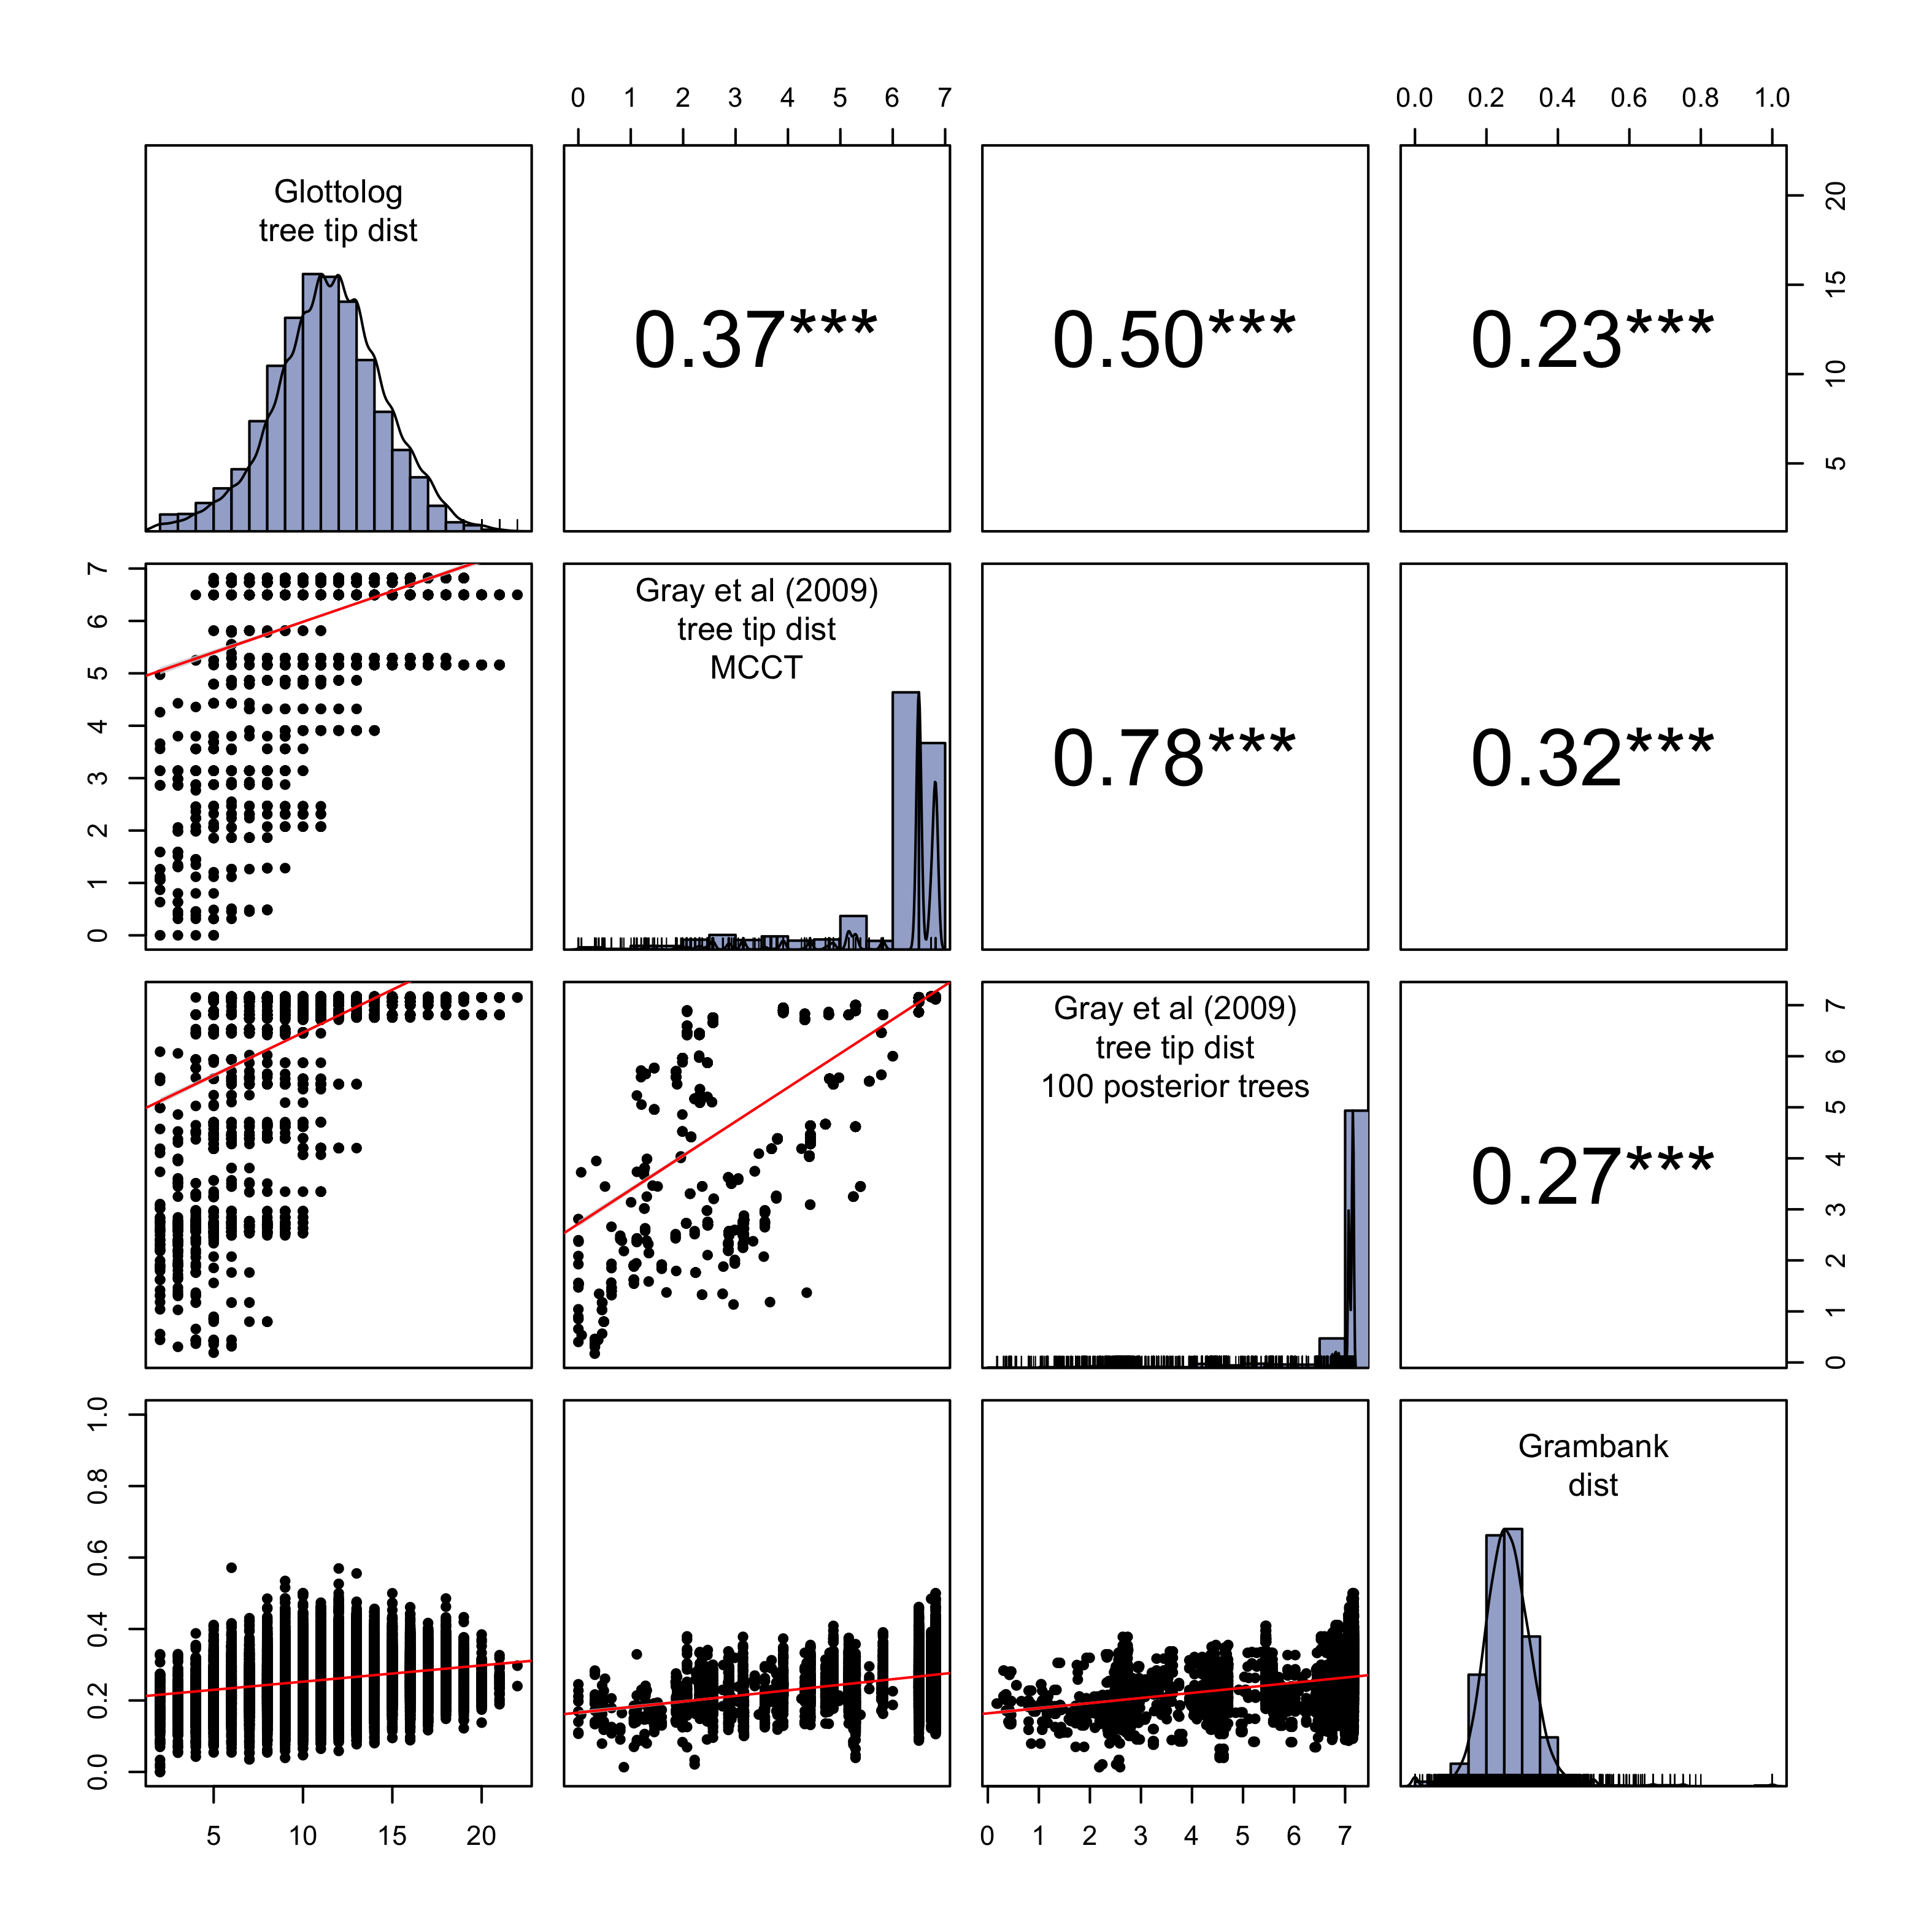
\includegraphics[width=17cm]{illustrations/plots_from_R/SPLOM_tree_dists.png}
\caption{Comparison of distances between tips of the different trees and Grambank. Correlations are Pearson coefficients, the stars indicate the conventional p-value cut-off at 0.05.}
\label{tree_dist_splom}
\end{figure}

\FloatBarrier
\newpage
\section{Supplementary Figure: tree heatmap of Gray et al (2009)-MCCT and Grambank variables}
\label{supp:fig_tree_heatmap}

Figure \ref{fig:tree_heatmap} shows the MCC-tree from \citet{grayetal_2009} and a data-matrix of all 201 binarised Grambank variables. These data are the input for the ASR-analysis for this particular tree and the D-estimate calculation. Missing data are ignored in both sets of analysis.

\begin{figure}[!ht]
\centering
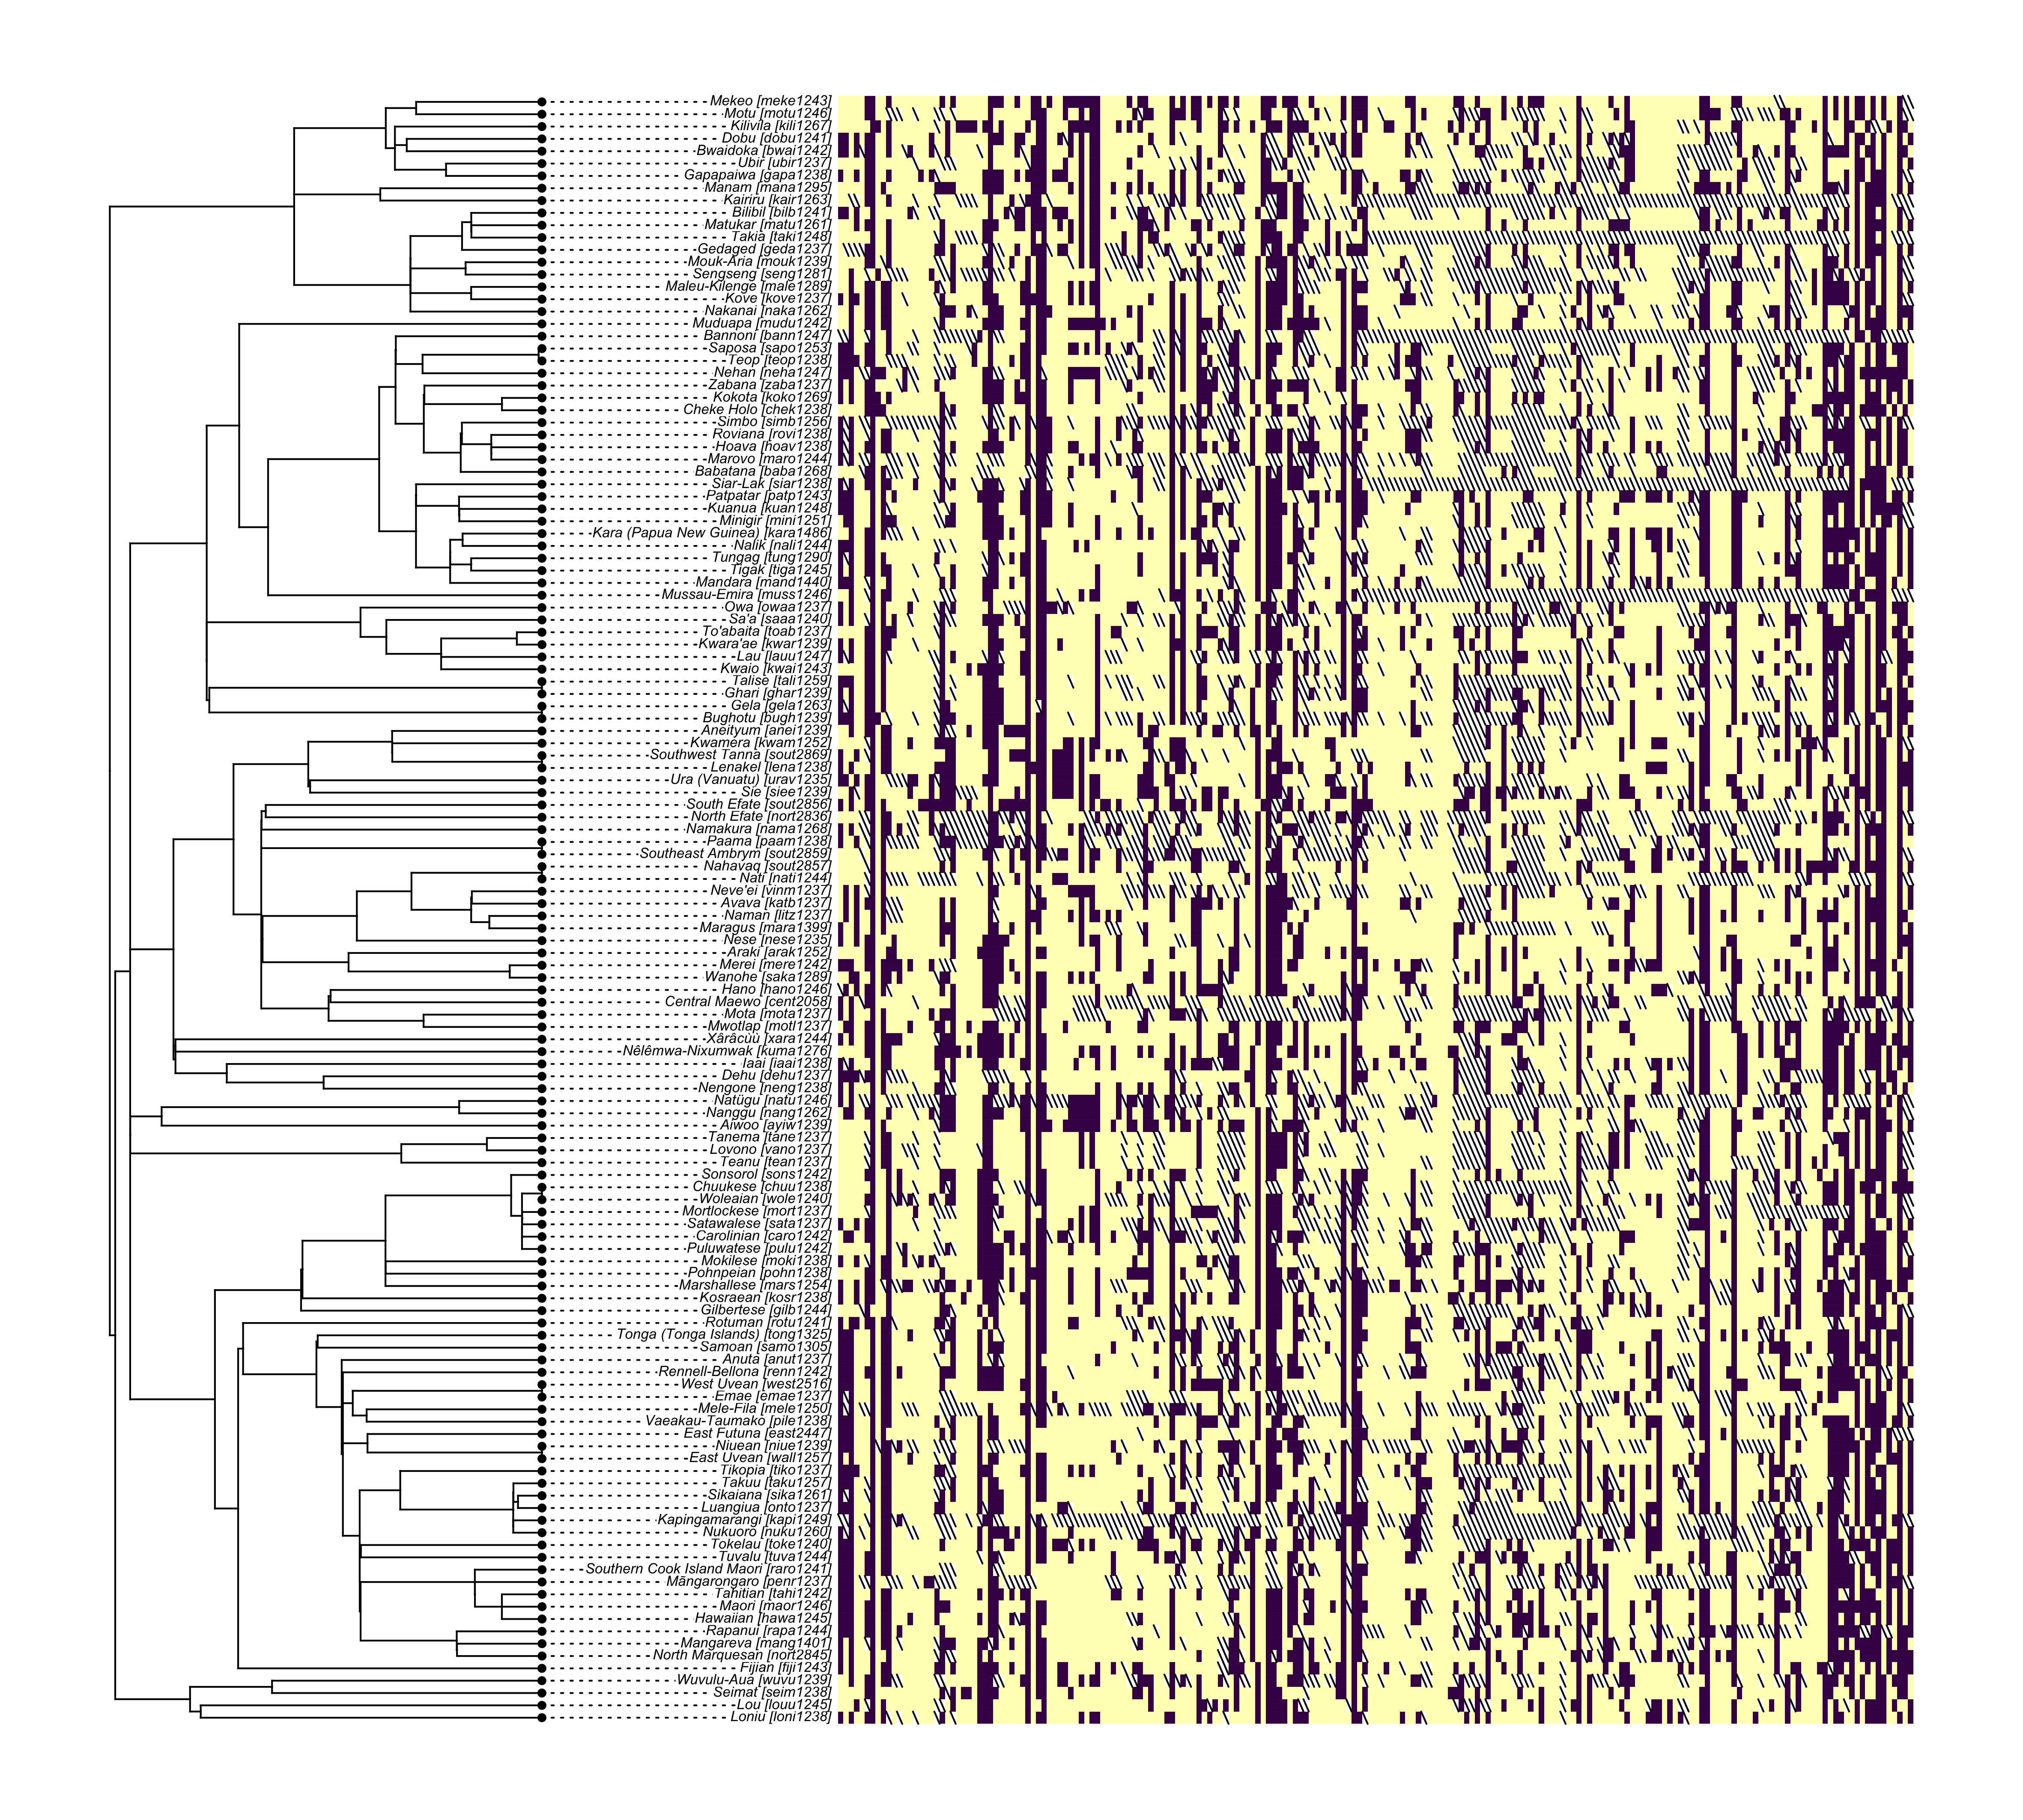
\includegraphics[width=18cm]{illustrations/plots_from_R/coverage_plots/tree_heatmap_gray_mcct.png}
\caption{MCC-tree from \citet{grayetal_2009} with Grambank data matrix. Purple = present, yellow = absent and striped = missing.}
\label{fig:tree_heatmap}
\end{figure}


\FloatBarrier
\newpage
\section{Technical details on D-estimation}
\label{supp:d_estimate}
D-estimates are a tool for measuring phylogenetic signal in a set of binary data. Phylogenetic signal can be broadly described as the degree to which the data are generated by a given tree, or whether it was generated by some other process such as randomness. This particular method was proposed by \cite{fritz2010selectivity} and is implemented in the R-package caper by Fritz and Orome \citep{orme2013caper}. 

The method outputs three primary values per dataset and tree: i) a D-estimate, ii) a p-value that represents how similar the data are to 0 (Brownian motion) and iii) the same kind of p-value, but instead in regard to how similar the data are to a D-estimate of 1 (randomness). If the 0-p-value is large (i.e., p>0.05) that means that the D-estimate of the data are \emph{not dissimilar} from 0, in other worse it is \emph{similar}. If we want to find sets of data that are similar to 0, we should look for large 0-p-values (not dissimilar = similar). The same goes for the p-values relating to 1. There can be D-estimates that are similar to both 0 \emph{and} 1 -- or neither.

The method relies on generating two kinds of simulated data: a Brownian threshold process and randomness. It then measures how similar your empirical data are to the Brownian simulation in comparison to how similar the Brownian simulation is to the random simulations. A D-estimate value of 0 represents identity to the Brownian process, 1 to the random process. D-estimates can also be smaller than 0 and larger than 1, and certainly any values in between. 

The results are sensitive to how many random permutations it runs for the second set of simulated data. \cite{fritz2010selectivity} recommends 1,000 permutations, which is also what the default value is set to for the function phylo.d in the R-package caper. However, during the work for this paper we have found further considerations that should be taken into account when working with this method -- specifically in regard to the number of random permutations and skewed distributions.

\subsection{D-estimate: Sensitivity to skewed distributions}
\label{sec:SM_phylo_d_sensitive}
While it is true that D-estimates can be smaller than 0 and larger than 1, in my experience values lower than -7 (very strong signal) and larger than 7 (very over-dispersed) are rare in empirical data. Furthermore, we would expect that if we re-run the algorithm a second time using the same data, same tree and same settings we get a similar result to the first time. This is generally true, except in certain specific situations. When the data are such that only one datapoint has a diverging value from the rest -- for example in a set of 155 tips only one of them has the value 1 for the binary trait and all others 0 -- then the algorithm struggles and produces very different results on each run, and very extreme values such as -10 on one run and 10 on another. This is problematic, and was probably not discovered by \cite{fritz2010selectivity} and \cite{orme2013caper} because their empirical data rarely exhibited this kind of distribution (1 - 154). However, for some of the linguistic features of this study this can indeed happen. 

Having identified the problem, we can also offer two solutions: a) increasing the number of random permutations and/or b) disregard data of this kind. Many thanks to \citep{orme2013caper} for the package documentation of caper and the paper by \cite{fritz2010selectivity} for providing enough methodological detail for this to be diagnosed. Stephen Mann was also invaluable to helping diagnose and address this issue mathematically.

To illustrate the problem I generated a tree with 155 tips with different distributions of binary values. The list below describes the different feature value distributions (with short names used in the plot in parenthesis) and Fig \ref{fig:phylo_d_heatmap} shows the tree and feature value distributions

\begin{itemize}
    \item only one tip of state 1, all other 154 tips 0 (singleton)
        \begin{itemize}
            \item daughter with few splits from the roots (outlier)
            \item in a more nested position (middle)
            \item at a random position (random)
        \end{itemize}
    \item three features with each a pair of direct sister tips of state 1, all other 153 tips 0 (sisters\_a, sisters\_b and sisters\_c)
    \item two random tips with the state 1, all other 0 (two\_random)
    \item three features with each a set of three closely related languages with the state 1, all other 152 tips 0 (triplets\_a, triplets\_b and triplets\_c)
    \item three random tips with the state 1, all other 0 (three\_random)
   \item three features with each a set of four closely related languages with the state 1, all other 151 tips 0 (quadruplets\_a, quadruplets\_b and quadruplets\_c
    \item four random tips with the state 1, all other 0 (four\_random)
    \item a cluster of 31 tips which form a clade all with 1 for the feature, all others 0 (cluster)
    \item 31 random tips with the same state, all others other (cluster\_random)
\end{itemize}

\begin{figure}[!ht]
\centering
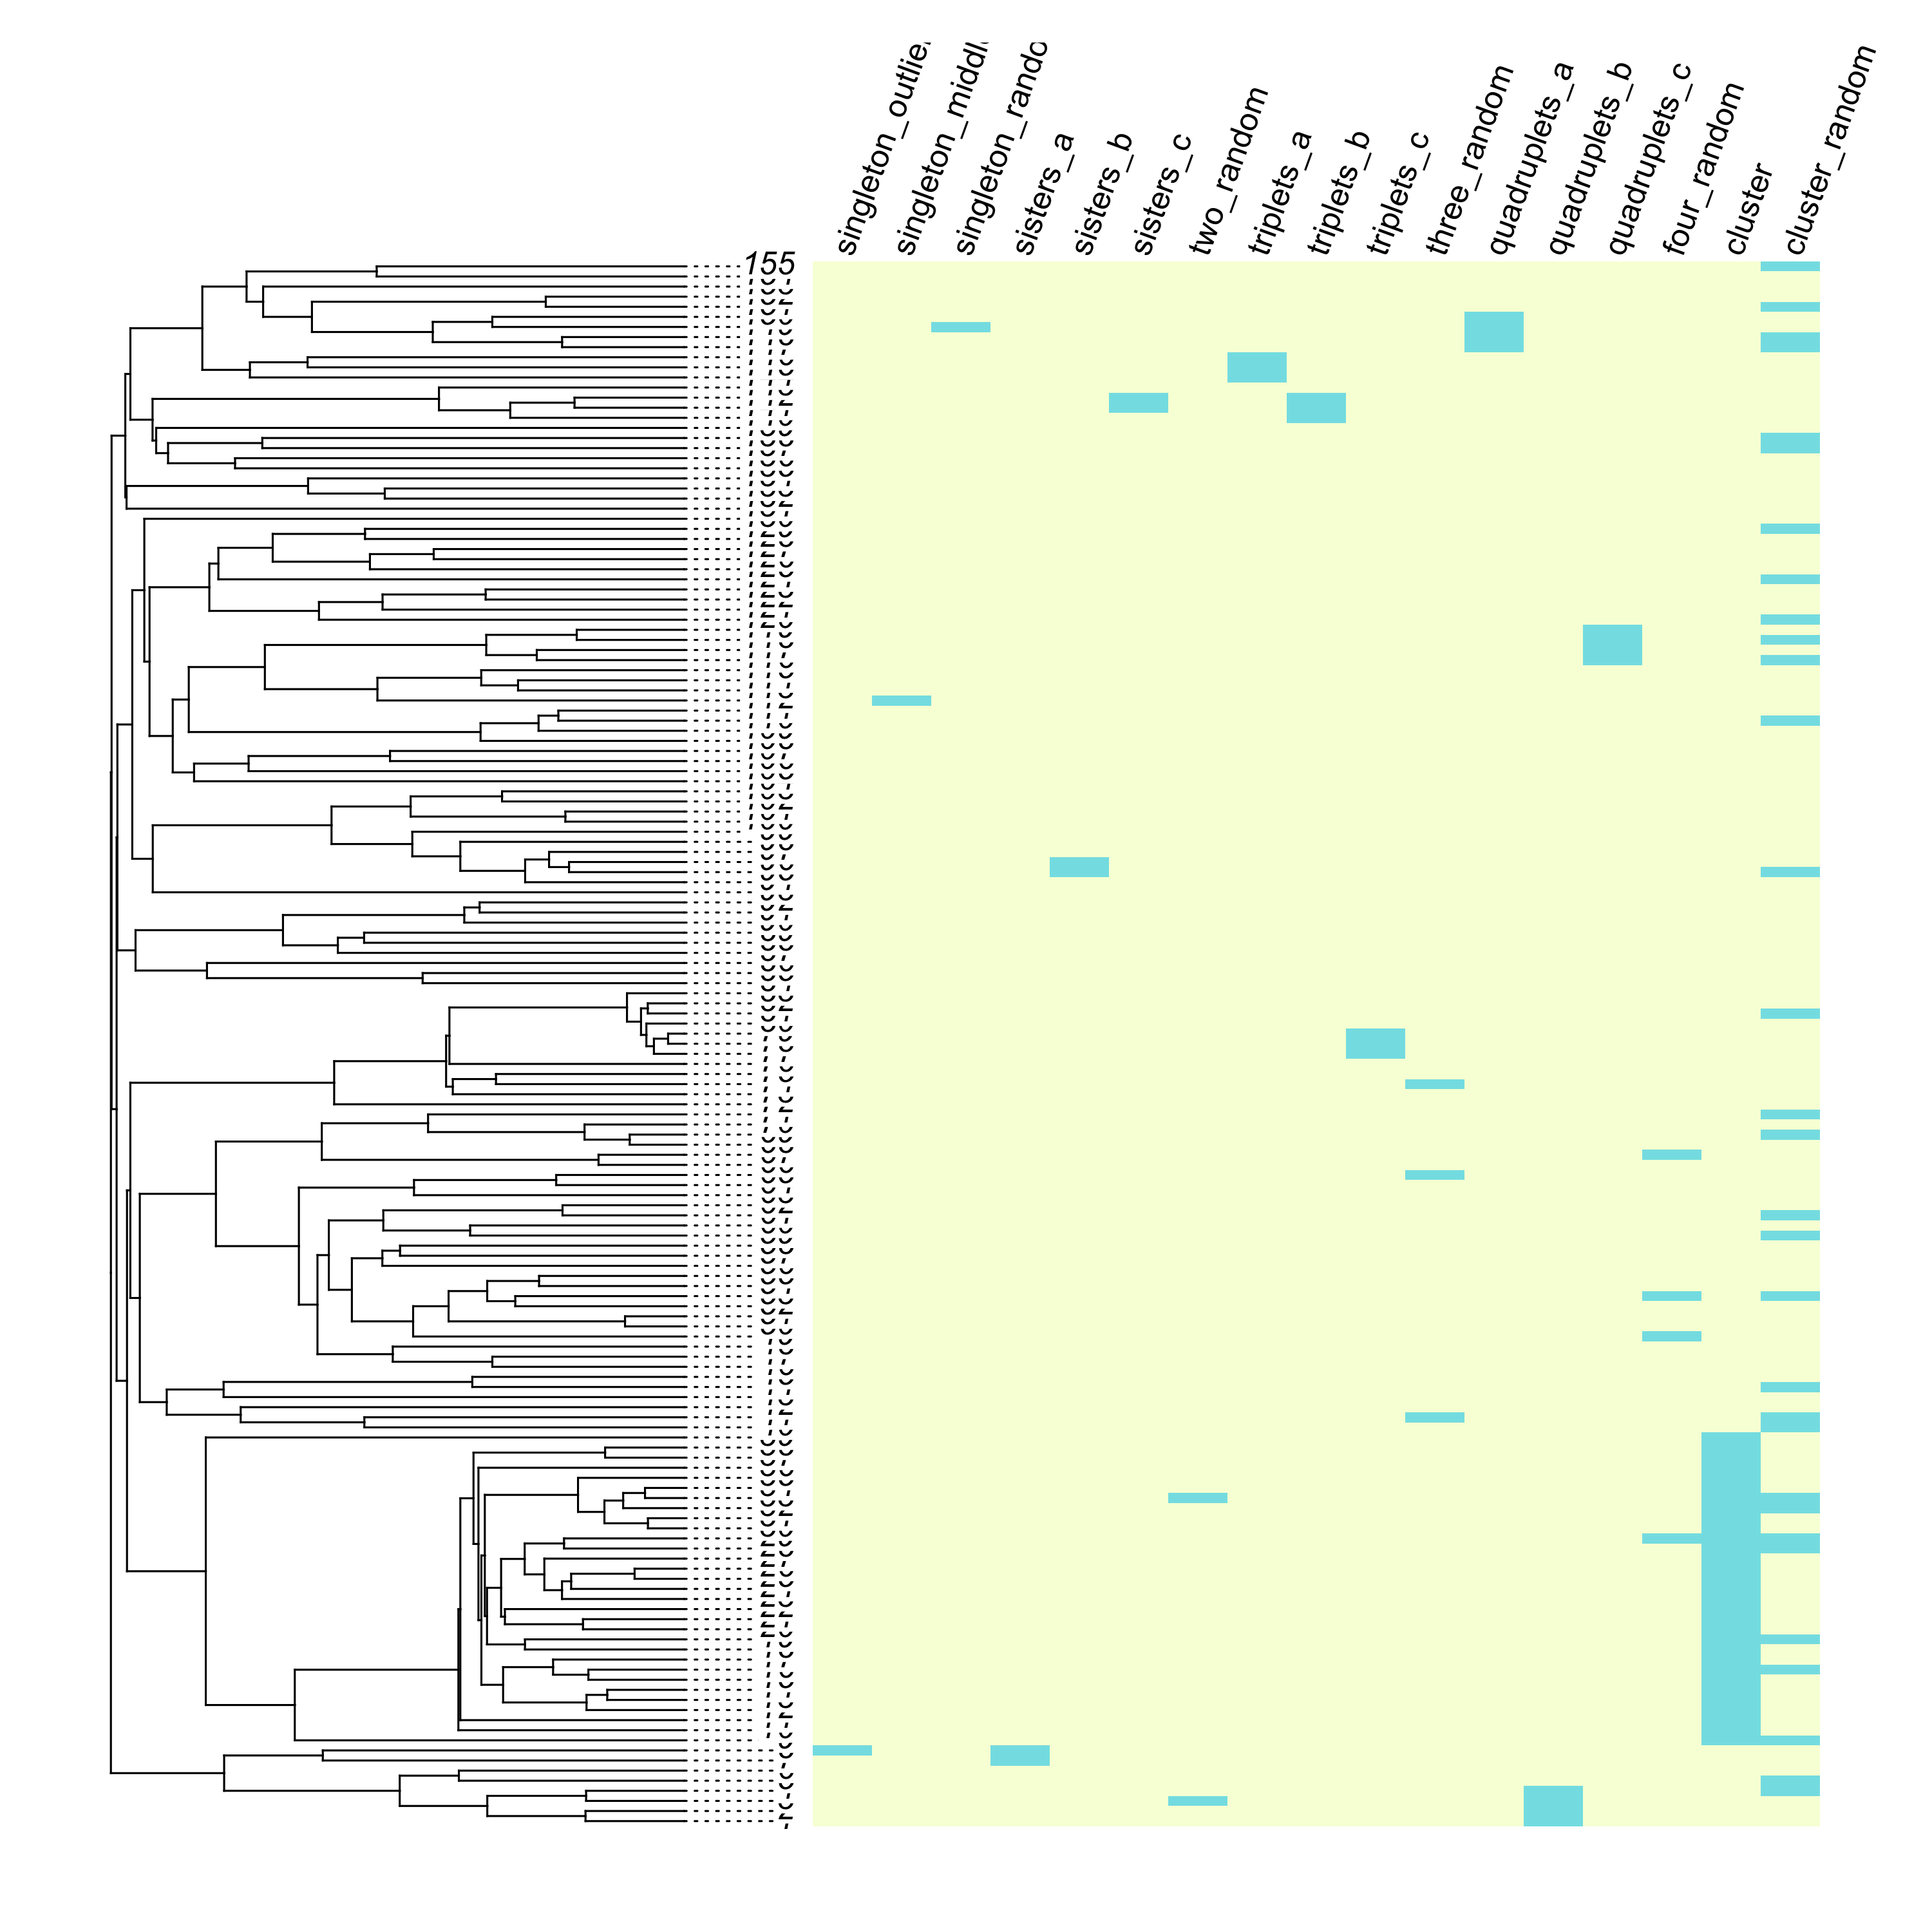
\includegraphics[width=14cm]{illustrations/plots_from_R/phylo_d_heatmap_tree.png}
\caption{Tree and values heatmap for D-estimation investigation.}
\label{fig:phylo_d_heatmap}
\end{figure}

I then proceeded to estimate the D-value for each of these 17 features, varying the number of permutations (1,000, 20,000 and 30,000). I repeated this 8 times, i.e., generating 17 * 3 * 8 D-estimates. For the entire investigation, see the script 11\_phylo\_d\_investigation.R in the accompanying material.

The D-estimates for the singleton-features varied the most, with one iteration of the singleton outlier feature reaching a D-estimate value of 1,520 (sic). This value occurred when the number of permutations was set to 1,000. In another iteration over the same feature and the same number of iterations, the D-estimate came out as -21. While it is potentially plausible to get very small or very large values, we would expect to get \emph{similar} values with each iteration given the same data and settings. The difference between a positive value of 1,520 and a negative of -21 is surely \emph{unreasonably} large. When the number of permutations was increased beyond 1,000, the variance of the output with each iteration was reduced (see Fig \ref{fig:phylo_d_plot_sd}), but it was still noticeably larger in cases where the distribution was heavily skewed.

\begin{figure}[!ht]
\centering
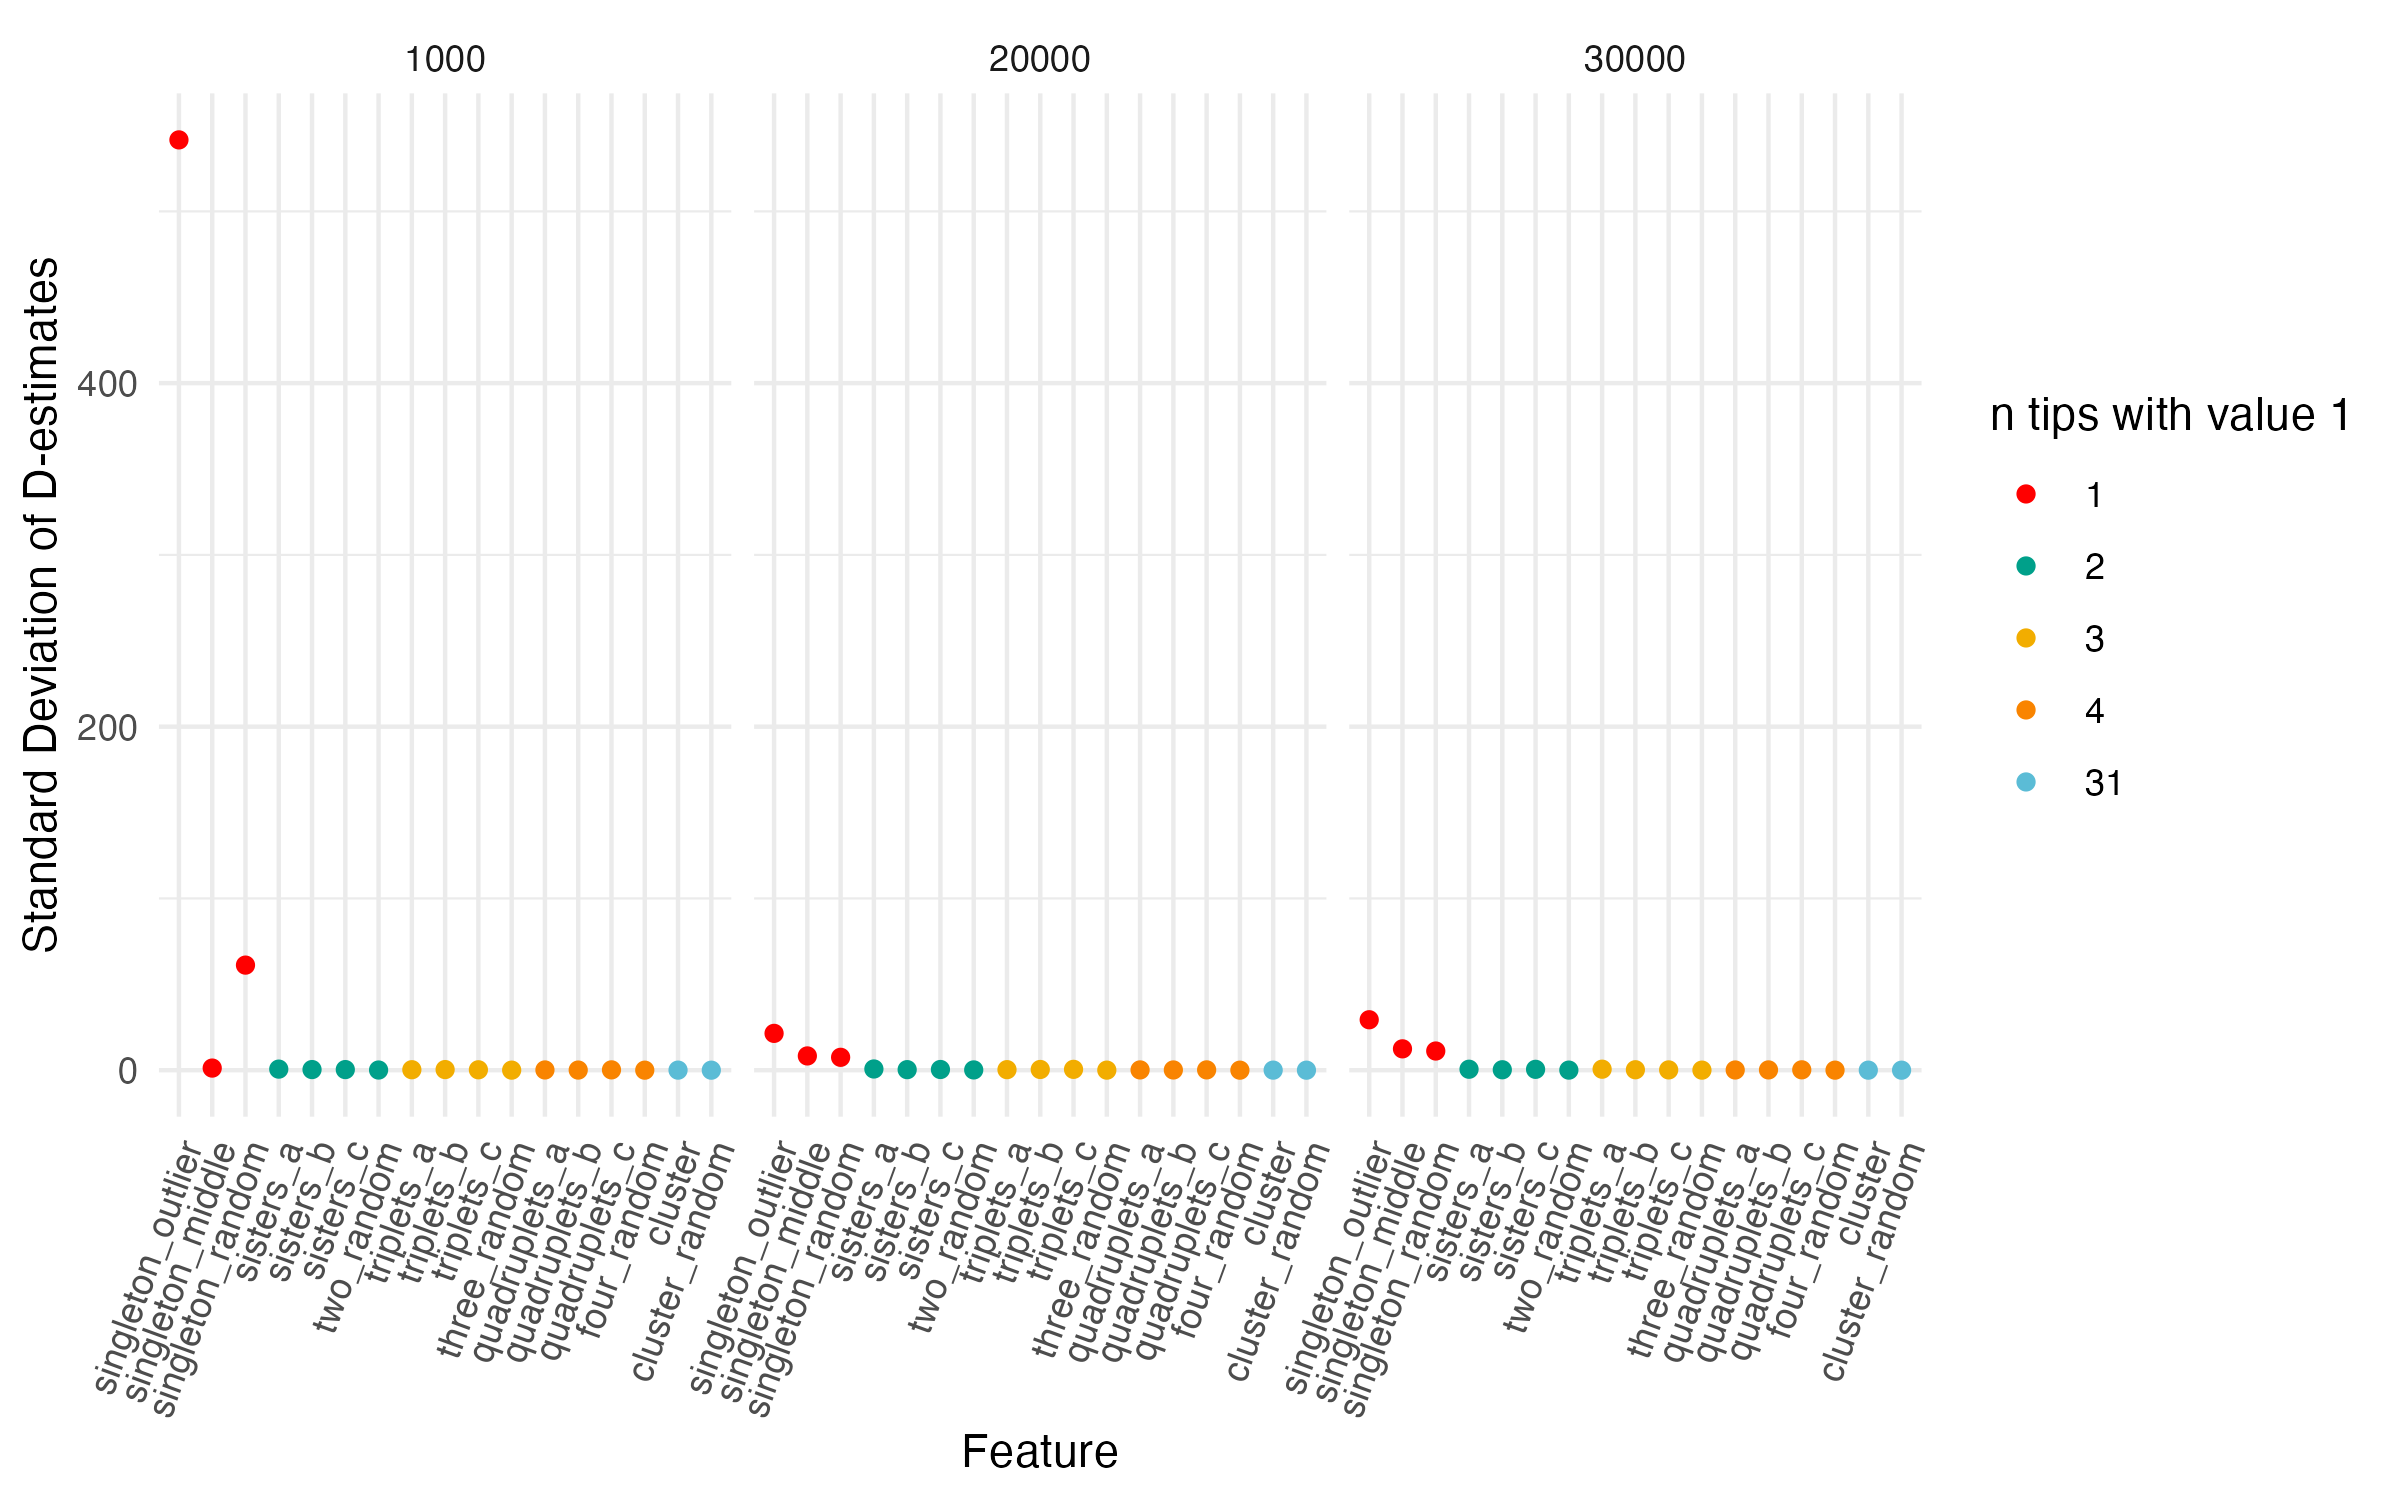
\includegraphics[width=14cm]{illustrations/plots_from_R/phylo_d_sd_permut.png}
\caption{Scatterplot of the standard deviation of D-estimate values per feature per value of random permutations}
\label{fig:phylo_d_plot_sd}
\end{figure}

The cause of this issue with wildly varying D-estimates each run, especially when the feature value distribution is very skewed, has to do with the chance of generating a particular pattern of 1/154 \emph{precisely} versus 4/151. Each time the D-estimate process is applied, a set of random and Brownian simulations are generated (the number is set by the permutations value). If the data are of the kind where 1 tip differs from all the other 154 tips (as for a few of the features in the toy example above), there is a chance that that particular position of that one value occurs in at least one of the random cases. If it does happen to occur, we would get a D-estimate that signals randomness -- and conversely if it happens to be similar to the Brownian evolutionary model. If the random and Brownian simulations end up being similar the denominator (see Eq. \ref{eq_d_estimate}) in the formula becomes very small, which can lead to very large absolute values for the D-estimate (such as the 1,520 we saw earlier). In Eq. \ref{eq_d_estimate}) \citep{fritz2010selectivity} r = random, b = brownian and obs = observed data.

\begin{align}
\label{eq_d_estimate}
    \text{D} 
         &=  \frac{\sum\emph{d}_{obs} - mean(\sum\emph{d}_{b})} {mean(\sum\emph{d}_{r}) - mean(\sum\emph{d}_{b})}
\end{align}

There is less of a chance of this happening if we have more tips in each state, because those are more complicated patterns that are less likely to occur exactly in the simulated processes. Because of the possibility of this irrelevant similarity, it is necessary to increase the number of simulated permutations so that we have a larger pool of things to compare our data to. This is why the D-estimate standard deviation stabilise more in cases with skewed feature distributions if the number of permutations is increased (see Fig \ref{fig:phylo_d_plot_sd}).

%The Brownian, observed and random distributions of values are more likely to happen to be similar the more skewed the feature value distribution is, as was said earlier it is easier to happen to have 1 value out of 155 in the same positions in a tree than, for example, 54 values. There are more unique configurations of a 54 - 101 value distribution over the tips than 1 - 154.

Even when the number of permutations is increased to 30,000, the instances where there is a feature distribution of 1 - 154 (singeltons) are more volatile than the rest. When using this technique, it may be necessary to set aside such cases and evaluate them separately from the rest. We may want to ask ourselves: what does it mean for something that does not even form a pair to have or not have a phylogenetic signal?

If we look at the non-singleton features (the pairs, triplets, quadruplets and larger group) in the simulation example explored here in Figure \ref{fig:phylo_d_plot_non_singles} we see that they behave more similarly with each iteration. Even an increase from 1 to 2 tips of the same state improves the performance of this method in terms of producing a similar value each iteration.

\begin{figure}[ht]
\centering
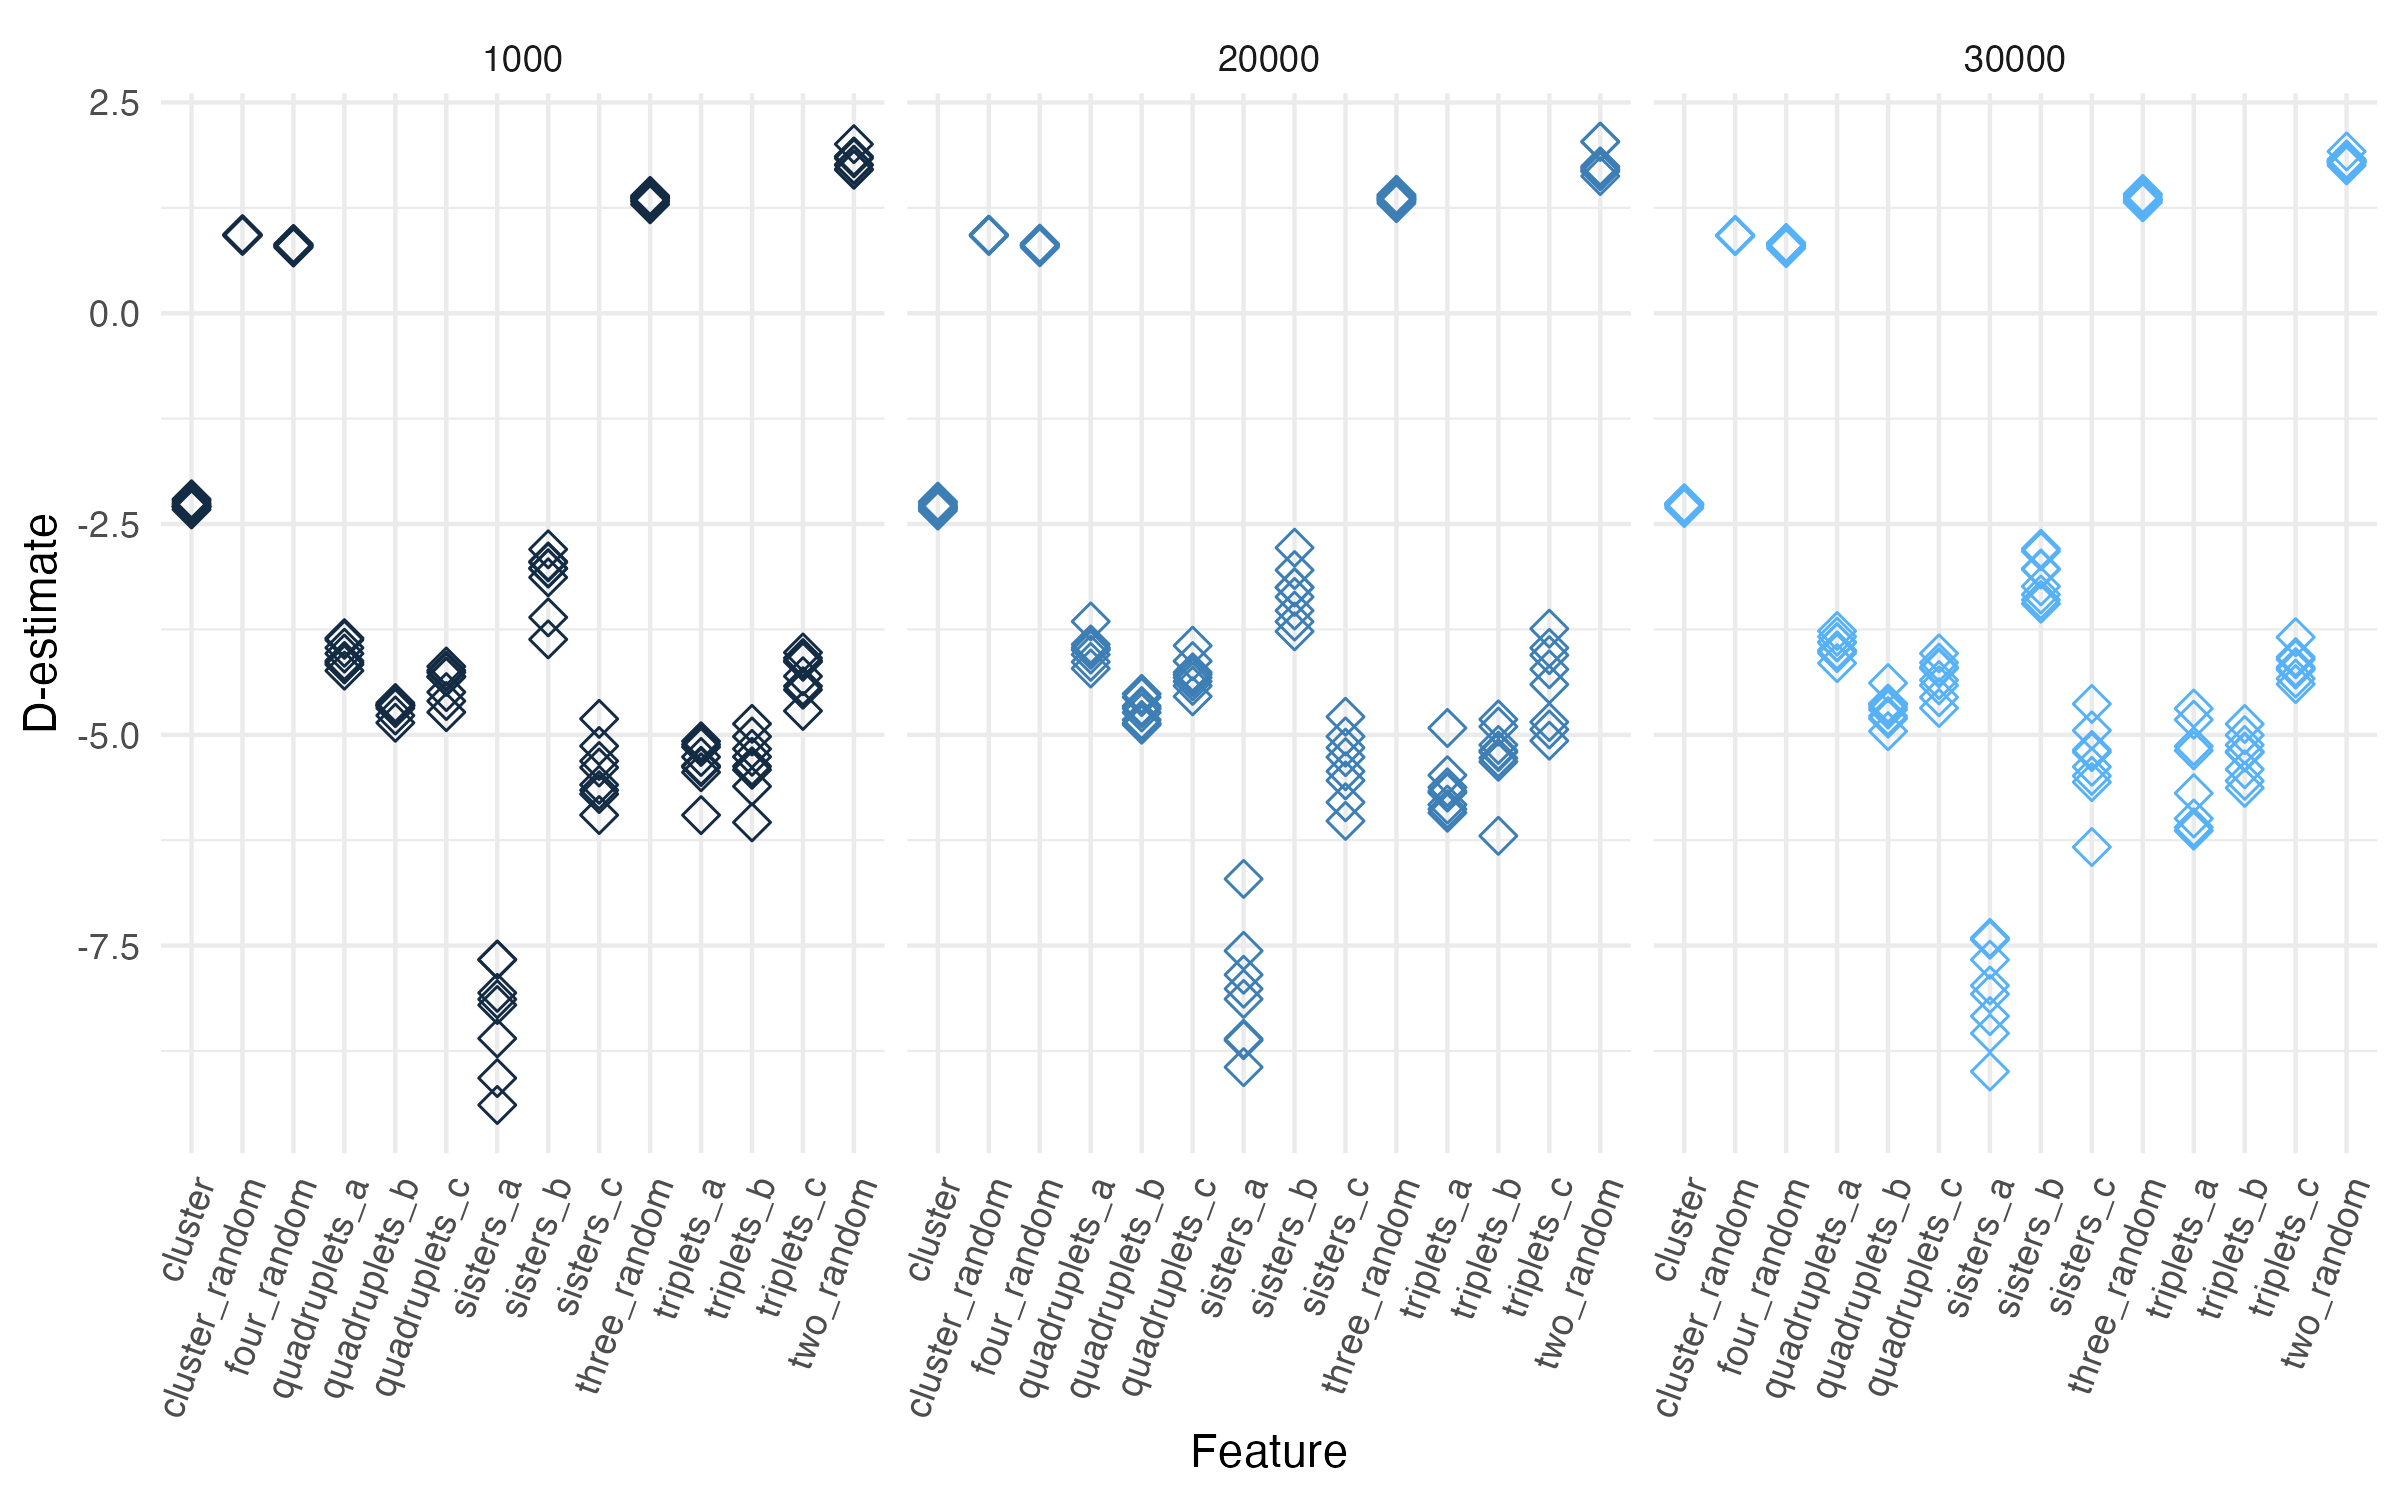
\includegraphics[width=14cm]{illustrations/plots_from_R/phylo_d_permut_plot.png}
\caption{Scatterplot of the D-estimate values per feature per value of random permutations, for all non-singleton features. Each point represents a D-estimate value per feature, per number of permutations and per iteration.}
\label{fig:phylo_d_plot_non_singles}
\end{figure}

\subsection{Categories of D-estimates that do not meet the rigours of the model}
\label{sec:d_estimate_summaries}
In the data in this study, there were cases of inappropriate D-estimates, which were possible to diagnose both by the extremity of the D-estimates, but also by examining the p-values (dissimilarity to Brownian/clumped and random/over-dispersed). 

The output is grouped into 2 groups, with 3 subgroups each. The output in the second group is not possible to include in the analysis because the conditions do not meet the model requirements, it is either impossible to conduct the analysis (all tips one state), would generate seriously unreliable results (singleton states) or shows evidence of Brownian and random being similar which also throw suspicion on the outcome. For future work, it would be desirable if the \texttt{R-function caper::phylo.d()} also output a p-value which represents the dissimilarity between the random and Brownian simulations and in addition generated a warning when the distributions are heavily skewed (for example, only 5\% tips in one state). 

As with the ASR-results, I also excluded output where the number of tips that had data were fewer than half of the tips in the full Oceanic-tree, i.e., for Glottolog fewer than 135.5 and for the \cite{grayetal_2009}-trees 66. See counts in table \ref{d_estimate_summary} in §\ref{sec:is_it_valid}. The tables below only represent the D-estimates 

The p-values that are produced by the \texttt{R-function caper::phylo.d()} represent the proportion of simulations where the observed values had a smaller sum sister-clade differences compared to the Brownian simulation, and larger than the random. Pval0 = 0 means that the observed sister-clade differences were always greater than the Brownian simulations, pval0 = 1 means they were always lower. Pval1 = 0 means that the observed sister-clade differences were always lower than the random simulations, and pval1 = 1 means that they were always greater than the random.  For more details, see the source code of \texttt{caper::phylo.d()}.

\begin{itemize}
    \item \colorbox{spec_color_lightgreen!50}{possible to include in analysis}
    \begin{enumerate}[label=(\roman*)]
     \item observed values definitely on the Brownian/clumped end of the spectrum (pval0 > 0.05 \& pval1 < 0.05)
      \item observed values definitely on the random/overdispersed end of the spectrum (pval0 < 0.05 \& pval1 > 0.05)
      \item observed values definitely between Brownian/clumped and random/over-dispersed. In all of these cases, the D-estimate is between 0 and 1. (pval0 < 0.05 \& pval1 < 0.05)
    \end{enumerate}
    \item \colorbox{spec_color_orange!50}{\emph{not} possible to include in analysis}
    \begin{enumerate}[label=(\roman*)]
        \item all tips same state (D-estimate is undefined)
        \item singleton (only one tip has a different state from all other tips)
        \item Brownian and random simulations are not sufficiently distinct from each other to get a meaningful D-estimate, observed values appear to be similar to both (pval0 > 0.05 \& pval1 > 0.05). D-estimate can be <0, in between or >1.
    \end{enumerate}
    
\end{itemize}

Tables \ref{phylo_d_summarise_col_green} and \ref{phylo_d_summarise_col_orange} shows the number of instances of each of these categories over the trees. There are fewer instances in the problematic categories and they have been excluded from further analysis with D-estimates. Because they represent cases with skewed distributions, it is possible to interpret them as representing very rare phenomena and one interpretation of that could be a strong phylogenetic signal -- but the D-estimate test is not suitable. The values for the 100 trees from the posterior are averages.

% latex table generated in R 4.2.2 by xtable 1.8-4 package
% Wed Mar 15 22:58:17 2023
\begin{table}[ht]
\centering
\begin{tabular}{p{3cm}p{3cm}p{3cm}p{3cm}p{3cm}}
  \toprule
tree & $\textbf{\cellcolor{spec_color_lightgreen!50}{\parbox{2.7cm}{\raggedright similar to 0}}}$ & $\textbf{\cellcolor{spec_color_lightgreen!50}{\parbox{2.7cm}{\raggedright similar to both, between 0 \& 1}}}$ & $\textbf{\cellcolor{spec_color_lightgreen!50}{\parbox{2.7cm}{\raggedright similar to 1}}}$ & $\textbf{\cellcolor{spec_color_lightgreen!50}{\parbox{2.7cm}{\raggedright dissimilar to both, between 0 \& 1}}}$ \\ 
  \midrule
glottolog & 59 & 9 & 28 & 75 \\ 
  Gray (2009) - mcct & 76 & 23 & 44 & 20 \\ 
  Gray (2009) - posteriors & 89 & 37 & 24 & 2 \\ 
   \bottomrule
\end{tabular}
\caption{Table of types of D-estimates per tree, data-points included.} 
\label{phylo_d_summarise_col_green}
\end{table}


% latex table generated in R 4.2.2 by xtable 1.8-4 package
% Thu Jan 26 14:56:37 2023
\begin{table}[h]
\centering
\begin{tabular}{p{3cm}p{3cm}p{3cm}p{3cm} p{3cm}}
  \toprule
tree & $\textbf{\cellcolor{spec_color_orange!50}{\parbox{2.7cm}{\raggedright all same}}}$ & $\textbf{\cellcolor{spec_color_orange!50}{\parbox{2.7cm}{\raggedright one off}}}$ & $\textbf{\cellcolor{spec_color_orange!50}{\parbox{2.7cm}{\raggedright similar to both, above 1}}}$ & $\textbf{\cellcolor{spec_color_orange!50}{\parbox{2.7cm}{\raggedright similar to both, below 0}}}$ \\ 
  \midrule
glottolog & 0 & 2 & 2 & 1 \\ 
  Gray (2009) - mcct & 1 & 3 & 2 & 4 \\ 
  Gray (2009) - posterior & 1 & 3 & 2 & 7 \\ 
   \bottomrule
\end{tabular}
\caption{Table of types of D-estimates per tree, data-points not included.} 
\label{phylo_d_summarise_col, orange}
\end{table}



%#todo
\FloatBarrier


\subsection{Correlation D-estimate and HL-concurrence}
\label{supp:cor_d_HL}
Phylogenetic signal could be an indication that it is easier to reconstruct a prior state. One may for example consider that it ought to be more difficult to reconstruct a state reliably if the pattern is a random phylogenetic signal (D-estimate similar to 1), and conversely that a strong signal may make it easier to reconstruct consistently, and therefore that the agreement between conventional historical linguistics findings and the computational methods applied in this paper would be higher if the phylogenetic signal is strong (=similar to 0, Brownian). This is however not the case in this study.

Figure \ref{fig:phylo_d_plot_vs_concurrence} shows the D-estimate on the x-axis (low = strong signal, high = random) and agreement with conventional historical linguistics on the y-axis. The agreement with HL is the precise value that the method predicted for the state that HL suggests. If HL suggests that the state is present at a particular node, and the computational suggests that presence has a likelihood of 0.435, the agreement value is 0.435. This is a continuous scale, but for the parsimony results it is often 0, 0.5 or 1 because of the prevalence of binary splits in the tree and the way the method works.

The results have been grouped by method and tree. In no case, save one, does the correlation reach the conventional threshold for statistical significance for the Pearson correlation (p > 0.05). The exception is Parsimony - Glottolog tree, and even there the correlation is weak (0.23). Furthermore, the correlation is positive which is the opposite of what we would expect. If strong phylogenetic signal (low D-estimate) predicts high agreement, then the correlation would be negative. 

\begin{figure}[ht]
\centering
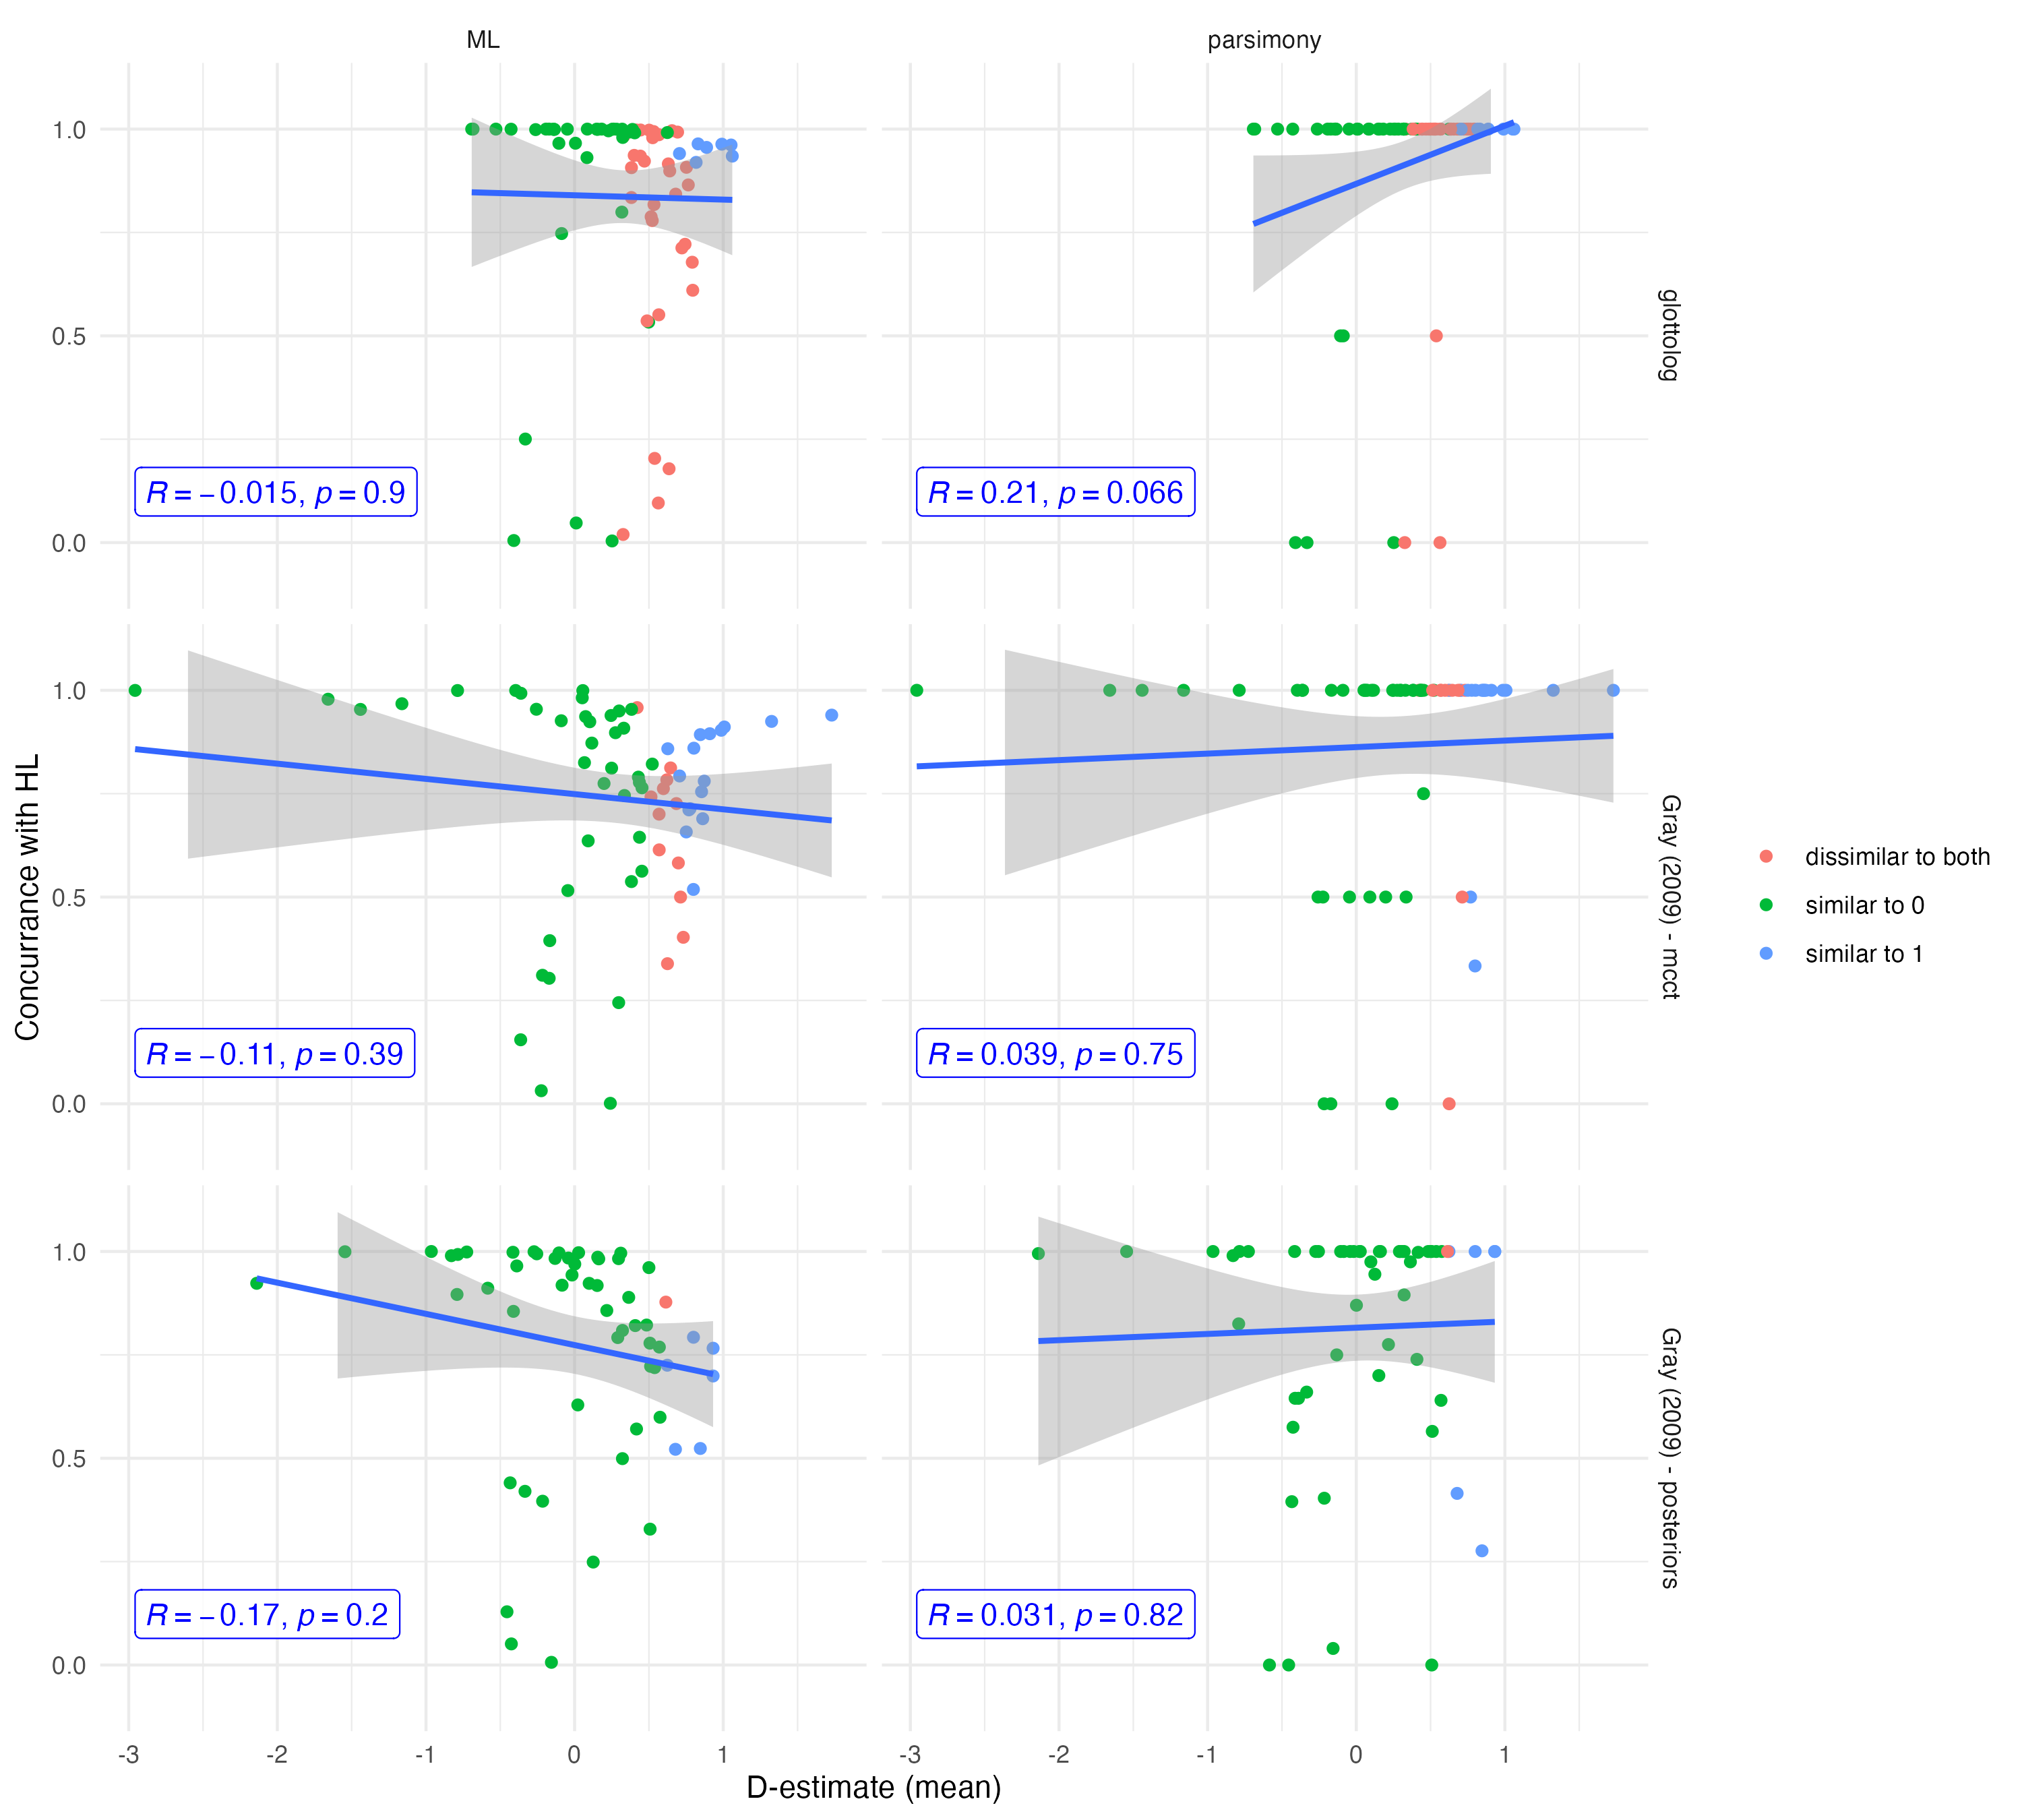
\includegraphics[width=18cm]{illustrations/plots_from_R/phylo_d_vs_HL_concurrance.png}
\caption{Scatter-plots of D-estimates (x-axis) and concurrence with conventional historical linguistics (y-axis). The points are coloured based on meeting statistical thresholds of significance for being similar to 0 (Brownian) or 1 (random). The correlation statistic in blue represents a Pearson-test.}
\label{fig:phylo_d_plot_vs_concurrence}
\end{figure}

Each point is mapped onto one prediction of one feature and one proto-language (Proto-Oceanic, Proto-Central Pacific, Proto-Polynesian or Proto-Eastern Polynesian), but the D-estimate is only taken for the entire Oceanic tree, not for each sub-clade. The predictions for "most common" were excluded, since there is not a tree \emph{per se} which the D-estimate can take as input to measure the phylogenetic signal. In addition, we also excluded datapoints that were ill-fitting for other reasons as discussed in the previous section.

\FloatBarrier

\section{Correlation value distributions and HL-concurrence}
\label{supp:cor_min_p_HL}
We can consider a much simpler approach to understanding what predicts agreement between the computational methods and historical linguists -- the number of tips in each state, then we see some stronger patterns. The idea is that if very few tips are in one state and all others in the other, there is little variation that can drive disagreements between the different reconstructions. If on the other hand, the states are distributed 50\%/50\% then it is reasonable to assume there is a greater chance for disagreement. In fig  \ref{fig:min_p_vs_concurrence}, the x-axis is the percentage of tips in the minority state -- 0\% indicates that all tips are of the same state (be that presence or absence) and 50\% that half of the tips are in one state, half in another. 30\% indicates that the state with the fewest tips had 30\% of the tips. The y-axis represents concurrence with traditional historical linguistics. Each point is one structural feature in one of the four proto-languages.

\begin{figure}[ht]
\centering
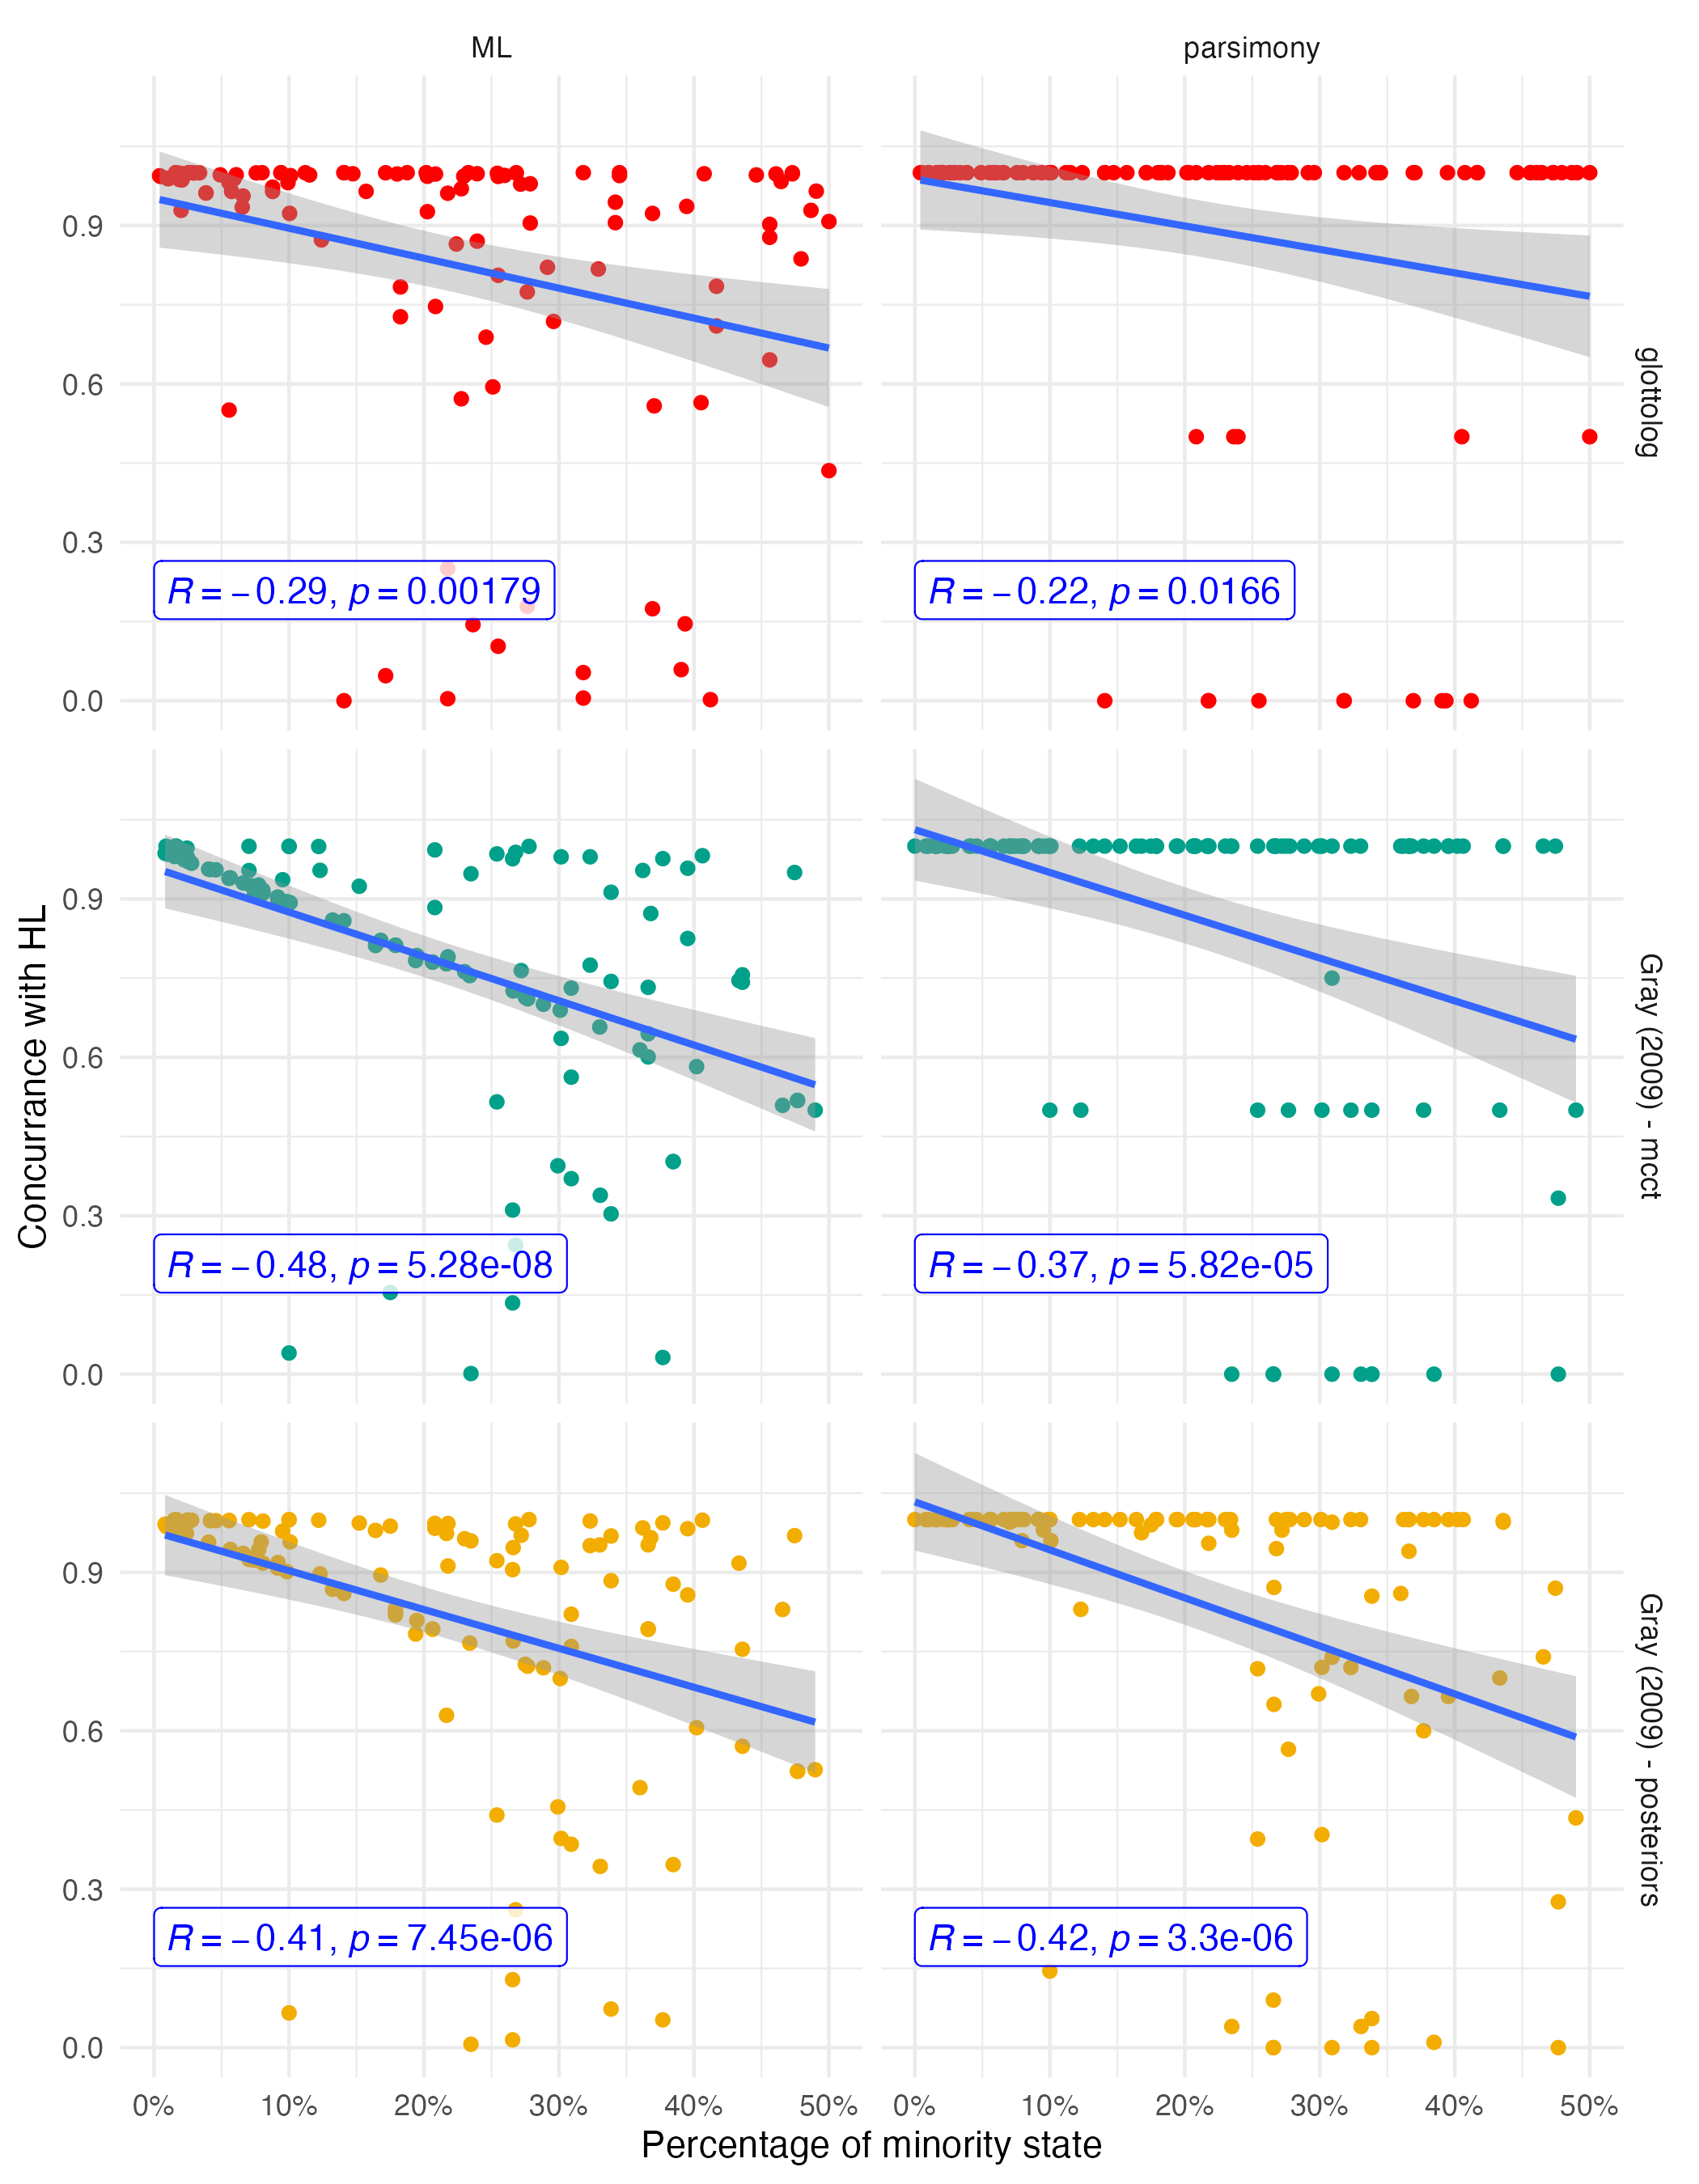
\includegraphics[width=12cm]{illustrations/plots_from_R/min_p_vs_HL_concurrance.png}
\caption{Scatter-plots of precentage of tips in minority state (x-axis) and concurrence with conventional historical linguistics (y-axis). The correlation statistic in blue represents a Pearson-test.}
\label{fig:min_p_vs_concurrence}
\end{figure}

All of the comparisons between HL-concurrence and the percentage of tips in minority state have a p-value lower than 0.05, which is a commonly used cut-off for significance. All correlations are negative, which is to be expected. This indicates that when tips are more evenly distributed between the two states (closer to 50\% on the x-axis), there is more disagreement between each of the methods and traditional HL. Most correlations are weak (between 0.2 and 0.39), and a few are of moderate strength (between 0.40 - 0.59). There are some outliers in the lower left quadrant of the plot, these represent cases where most tips are in one state and yet there is a disagreement. One of them is discussed in greater detail in the following section.

\FloatBarrier

\section{Disagreement between methods detail: present, 50\%/50\% versus absent}
\label{supp:GB133_detail}
One example of disagreement between conventional HL, Maximum Parsimony and Maximum Likelihood is GB133 `Is a pragmatically unmarked constituent order verb-final for transitive clauses?` for Proto-Oceanic. This feature has a very low concurrence with HL for the ML method (0.04) and \citep{grayetal_2009}) MCC-tree, despite the tip state distribution being 10\%/90\% which we saw in the previous section usually predicts high agreement.

Let us first consider the historical linguistics literature and the feature at hand. The coding of Proto-Oceanic as present for this feature according to conventional historical linguistics is based on the following passage from \citet{pawley1973some}:

\begin{quotation}
\noindent\emph{
Capell's suggestion that the SOV order found in many New Guinea Oceanic languages is the result of influence by Papuan (non-Austronesian) languages, almost all of which show SOV order, seems reasonable. }[..]\emph{
Still, the fact that the better-known SVO languages also tolerate certain other orders (for non- pronominal constituents) suggests that some variation occurred in POC} [Proto-Oceanic]\emph{. In particular, occurrences of OSV and VOS order are widely distributed enough to indicate that both were possible in POC.}\footnote{Pawley does note that the ``basic'' word order in Proto-Oceanic is likely to be SVO (Subject-Verb-Object).}
\end{quotation} \begin{flushright}\citet[118]{pawley1973some}\end{flushright}

Unlike the chapter in the World Atlas of Language Structures on order in the transitive clause \citep{wals-81}, the Grambank feature questionnaire does not ask about the ``dominant''-type, but has 3 different binary questions about the ``pragmatically unmarked'' order. 

{\small
\begin{itemize}
    \item GB131 Is a pragmatically unmarked constituent order verb-initial for transitive clauses?
    \item GB132 Is a pragmatically unmarked constituent order verb-medial for transitive clauses?
    \item GB133 Is a pragmatically unmarked constituent order verb-final for transitive clauses?
\end{itemize}

 }
 
It is possible for a language to be answered ``yes'' for more than one question if multiple orders occur (without changing the pragmatics). However, most Oceanic languages were still coded as absent for GB133. The Maximum Parsimony and Maximum Likelihood all disagree with conventional HL regarding GB133 for Proto-Oceanic - but in different ways.

Fig \ref{fig:parsimony_gray_mcct} shows the Ancestral Nodes of GB133 on the Gray et al (2009)-MCCT with the parsimony method, and Fig \ref{fig:ML_gray_mcct} the same tree but with the Maximum Likelihood method. These two tree figures have the same exact topology and tip states, they only vary in the reconstruction of internal nodes (proto-languages). In each of the figures, there is a set of languages at the bottom of the tree that are coded as "yes" for  GB133 and these are located on the island of New Guinea or nearby. Their location in the tree is such that they form a clade that is an early offshoot from the root. For the parsimony method, that means that even though most of the tips are of another state, this group carries a lot of weight. The parsimony method suggests that the state of the root, of Proto-Oceanic, is 50\%/50\%. However, the Maximum Likelihood method takes into account branch lengths and the overall tendency in the tree for the trait value "absent" to be stable (because it estimates asymmetric rates, unlike MP which assumes symmetric rates). This results in a ML-estimation of proto-Oceanic as overwhelmingly absent of verb-finality.

\begin{figure}[ht]
\centering
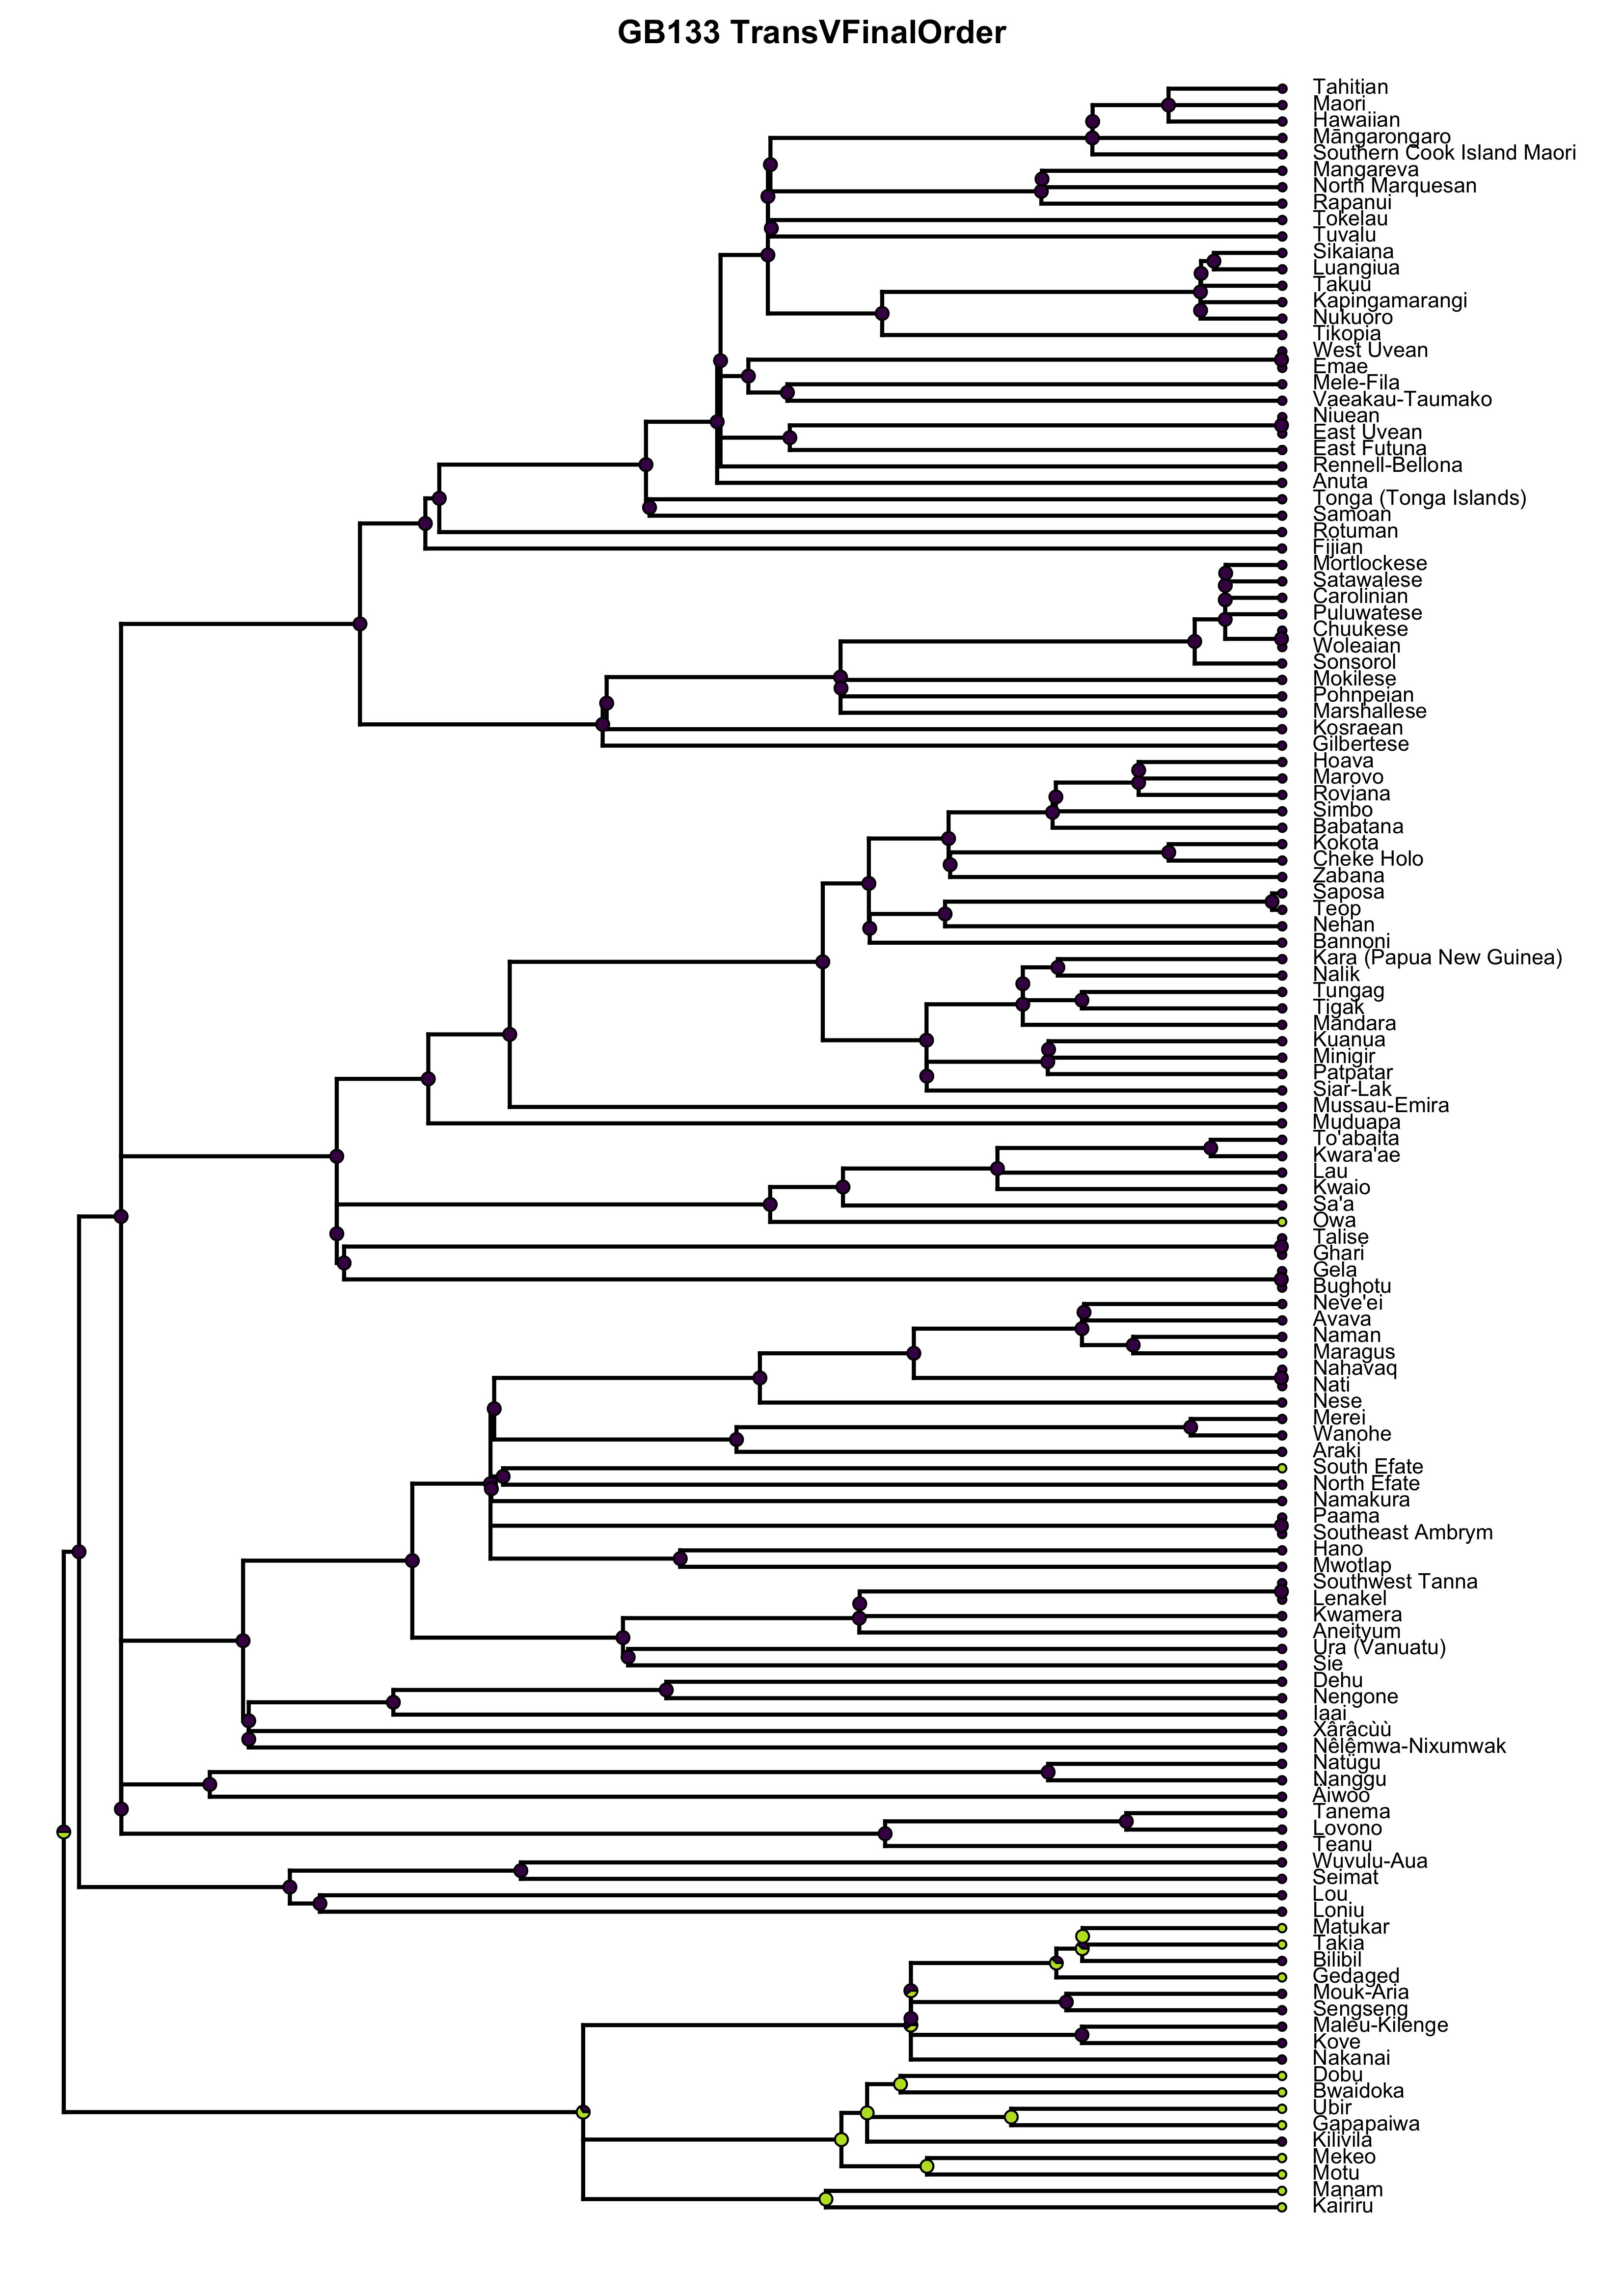
\includegraphics[width=14cm]{illustrations/plots_from_R/tree_plots/gray_et_al_2009/parsimony/parsimony_gray_tree_mcct_GB133.png}
\caption{Gray et al 2009-tree with Maximum Parsimony method, Proto-Oceanic is reconstructed as half/half present/absent. Green = absent, purple = present. Root edge added in for visualisation purposes only.}
\label{fig:parsimony_gray_mcct}
\end{figure}

\begin{figure}[ht]
\centering
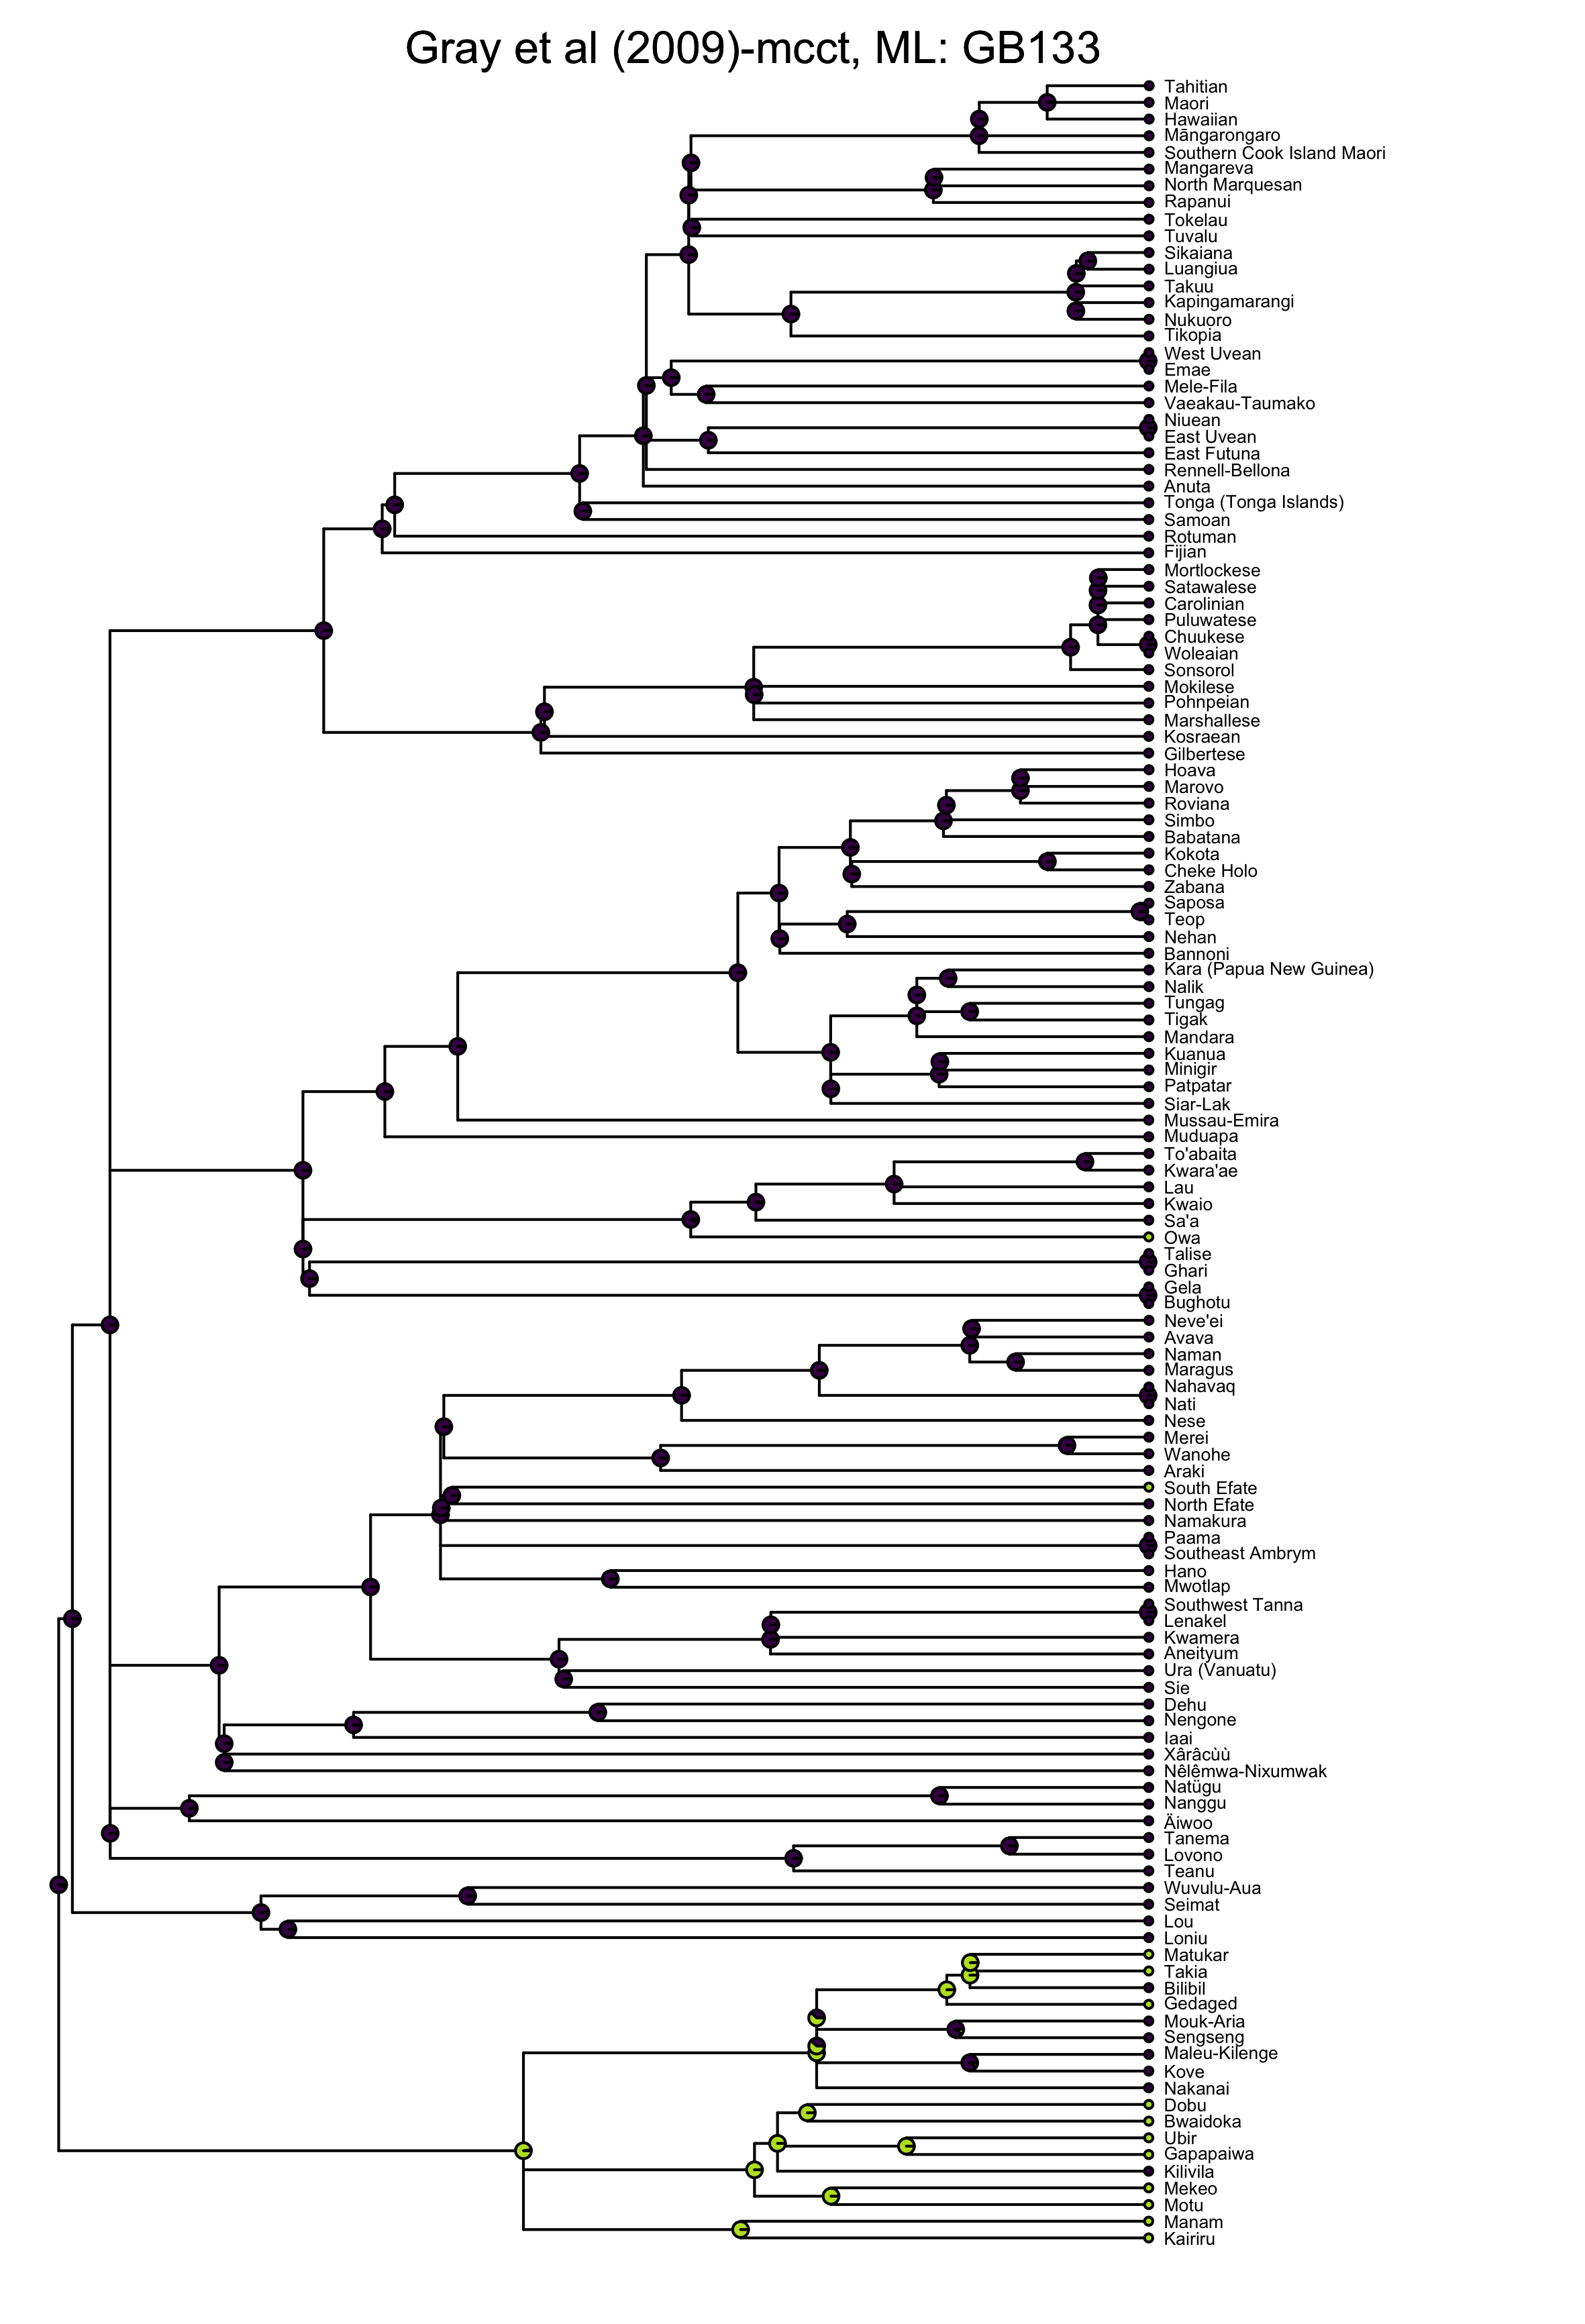
\includegraphics[width=14cm]{illustrations/plots_from_R/tree_plots/gray_et_al_2009/ML/ML_gray_mcct_-GB133.png}
\caption{Gray et al 2009-tree with ML method, Proto-Oceanic is reconstructed as absent.  Green = absent, purple = present. Root edge added in for visualisation purposes only.}
\label{fig:ML_gray_mcct}
\end{figure}

%
%



%Even when you set the number of permutations to 3000, the variation for cases where there is only one singleton tip is still pretty high (579 in my example), and the variance is also quite high for the cases of 2 and 4 cases compared to the case where a larger cluster exists.
%
%image
%If you want to dig deeper, there are also systematic differences if the singleton value is in a more or less direct daughter to the root (“outlier” in my code), smack in the middle or at a random position. It has to do with the way it does ancestral state reconstruction, which is through Felsenstein’s contrasting algorithm (sort of like max parsimony but smarter because it cares about branch lengths).
%
%The R-code I’ve uploaded doesn’t require you to download any data or anything, the tree and data are all there directly in the script. It doesn’t take that long time to run, and when it’s done it’ll do a little “pling!”. You can easily try it out and poke around yourself in the resulting data-frame.
%
%Solution
%
%If you are getting D-estimates that are varying wildly, first take a close look at your feature value distributions. Consider increasing the number of permutations to reign it in a bit.
%
%However, there’s something fundamental you need to consider if you’ve got very skewed data: in order for the D-measure to work, it needs groups of tips to latch onto, clumps. One tip is not a group. Two tips is better, but still a bit sus. You may want to disregard the D-estimates in such cases entirely, and separate those instances out in your data and compare and summarised them in a different way. Set them aside in one bucket and present them in some other way, and compare D-estimates of features that are more suited for this kind of analysis. Have a think about it, have a poke around - run the D-estimate many times and have a look at the variance you get.
%
%Good luck!
%
%P.S. Big thanks to my wonderfully smart husband Stephen (left below) for helping me work out the mathematics of all of this. He is a kind and intelligent person.

\FloatBarrier


\section{F1-score results}
\label{f1_results}

F1-scores are the harmonic mean of the precision and recall\footnote{Precision is True Positives divided by True Positives + False Positives, recall is True Positives divided by False Negatives + True Positives. F1-score = 2 * ((precision*recall) / (precision + recall)) \citep{van1979information}.} \citep[133]{van1979information}. It is important to note that F1-scores disregard the number of True Negatives entirely, which is relevant in our case since some of the features in proto-languages are predicted to be absent. For both measures, 0 is the worst possible score and 1 the best in terms of similarity to predictions by historical linguists. 

In a similar study of ancestral states of cognate classes, J\"ager and List (\citeyear{jager2018using}) compared three different methods of ancestral state reconstruction for lexical data (cognate classes): Maximum Parsimony, Maximum Likelihood and Minimal Lateral Networks. They found that reconstructions using Maximum Likelihood performed the most like the predictions by historical linguists. However, J\"ager and List (\citeyear{jager2018using}) describe the general performance of all the computational reconstruction methods they used as ``poor''. J\"ager and List (\citeyear{jager2018using}) evaluated the methods using the F1-score. The highest F1-score was 0.79 (Austronesian language sample, Maximum Likelihood), and the worst was 0.44 (Indo-European, Minimal Lateral Networks).

The formula for F1-scores is given in Eq. \ref{eq:F1_score}.

\begin{equation}\label{eq:F1_score}
\frac{\text{True Positive} }
{\text{True Positive} + \frac{1}{2}\times(\text{False Positive} + \text{False Negative})}
%\caption{Formula for F1-score}
\end{equation}

As stated in §\ref{result_calc_section}, the half-results are also interesting, the formula for F1-scores including half-results is given in Eq. \ref{eq:F1_score_incl_half}. For more on the caluclation of the F1-score including half results, see Supplementary Material \ref{math_supp}.

\begin{equation}\label{eq:F1_score_incl_half}
\frac{\text{True Positive} +  \frac{\text{Half}}{2}} 
{\text{True Positive} + \frac{1}{2}\times(\text{False Positive} + \text{False Negative}) + \text{Half}}
%\caption{Formula for F1-score including half-results}
\end{equation}

The results of the F1-scores are shown in Fig \ref{barplot_facet_results_incl_f1}, alongside the concordance scores. The result for the plain F1-score differs from the other three, this is precisely because it ignores True Negatives. While True Negatives are not included \emph{per se} in the calculation of F1 including half-results score, the inclusion of the half-similarity still has an impact as it makes all the methods more similar.

\begin{figure}[p]
\centering
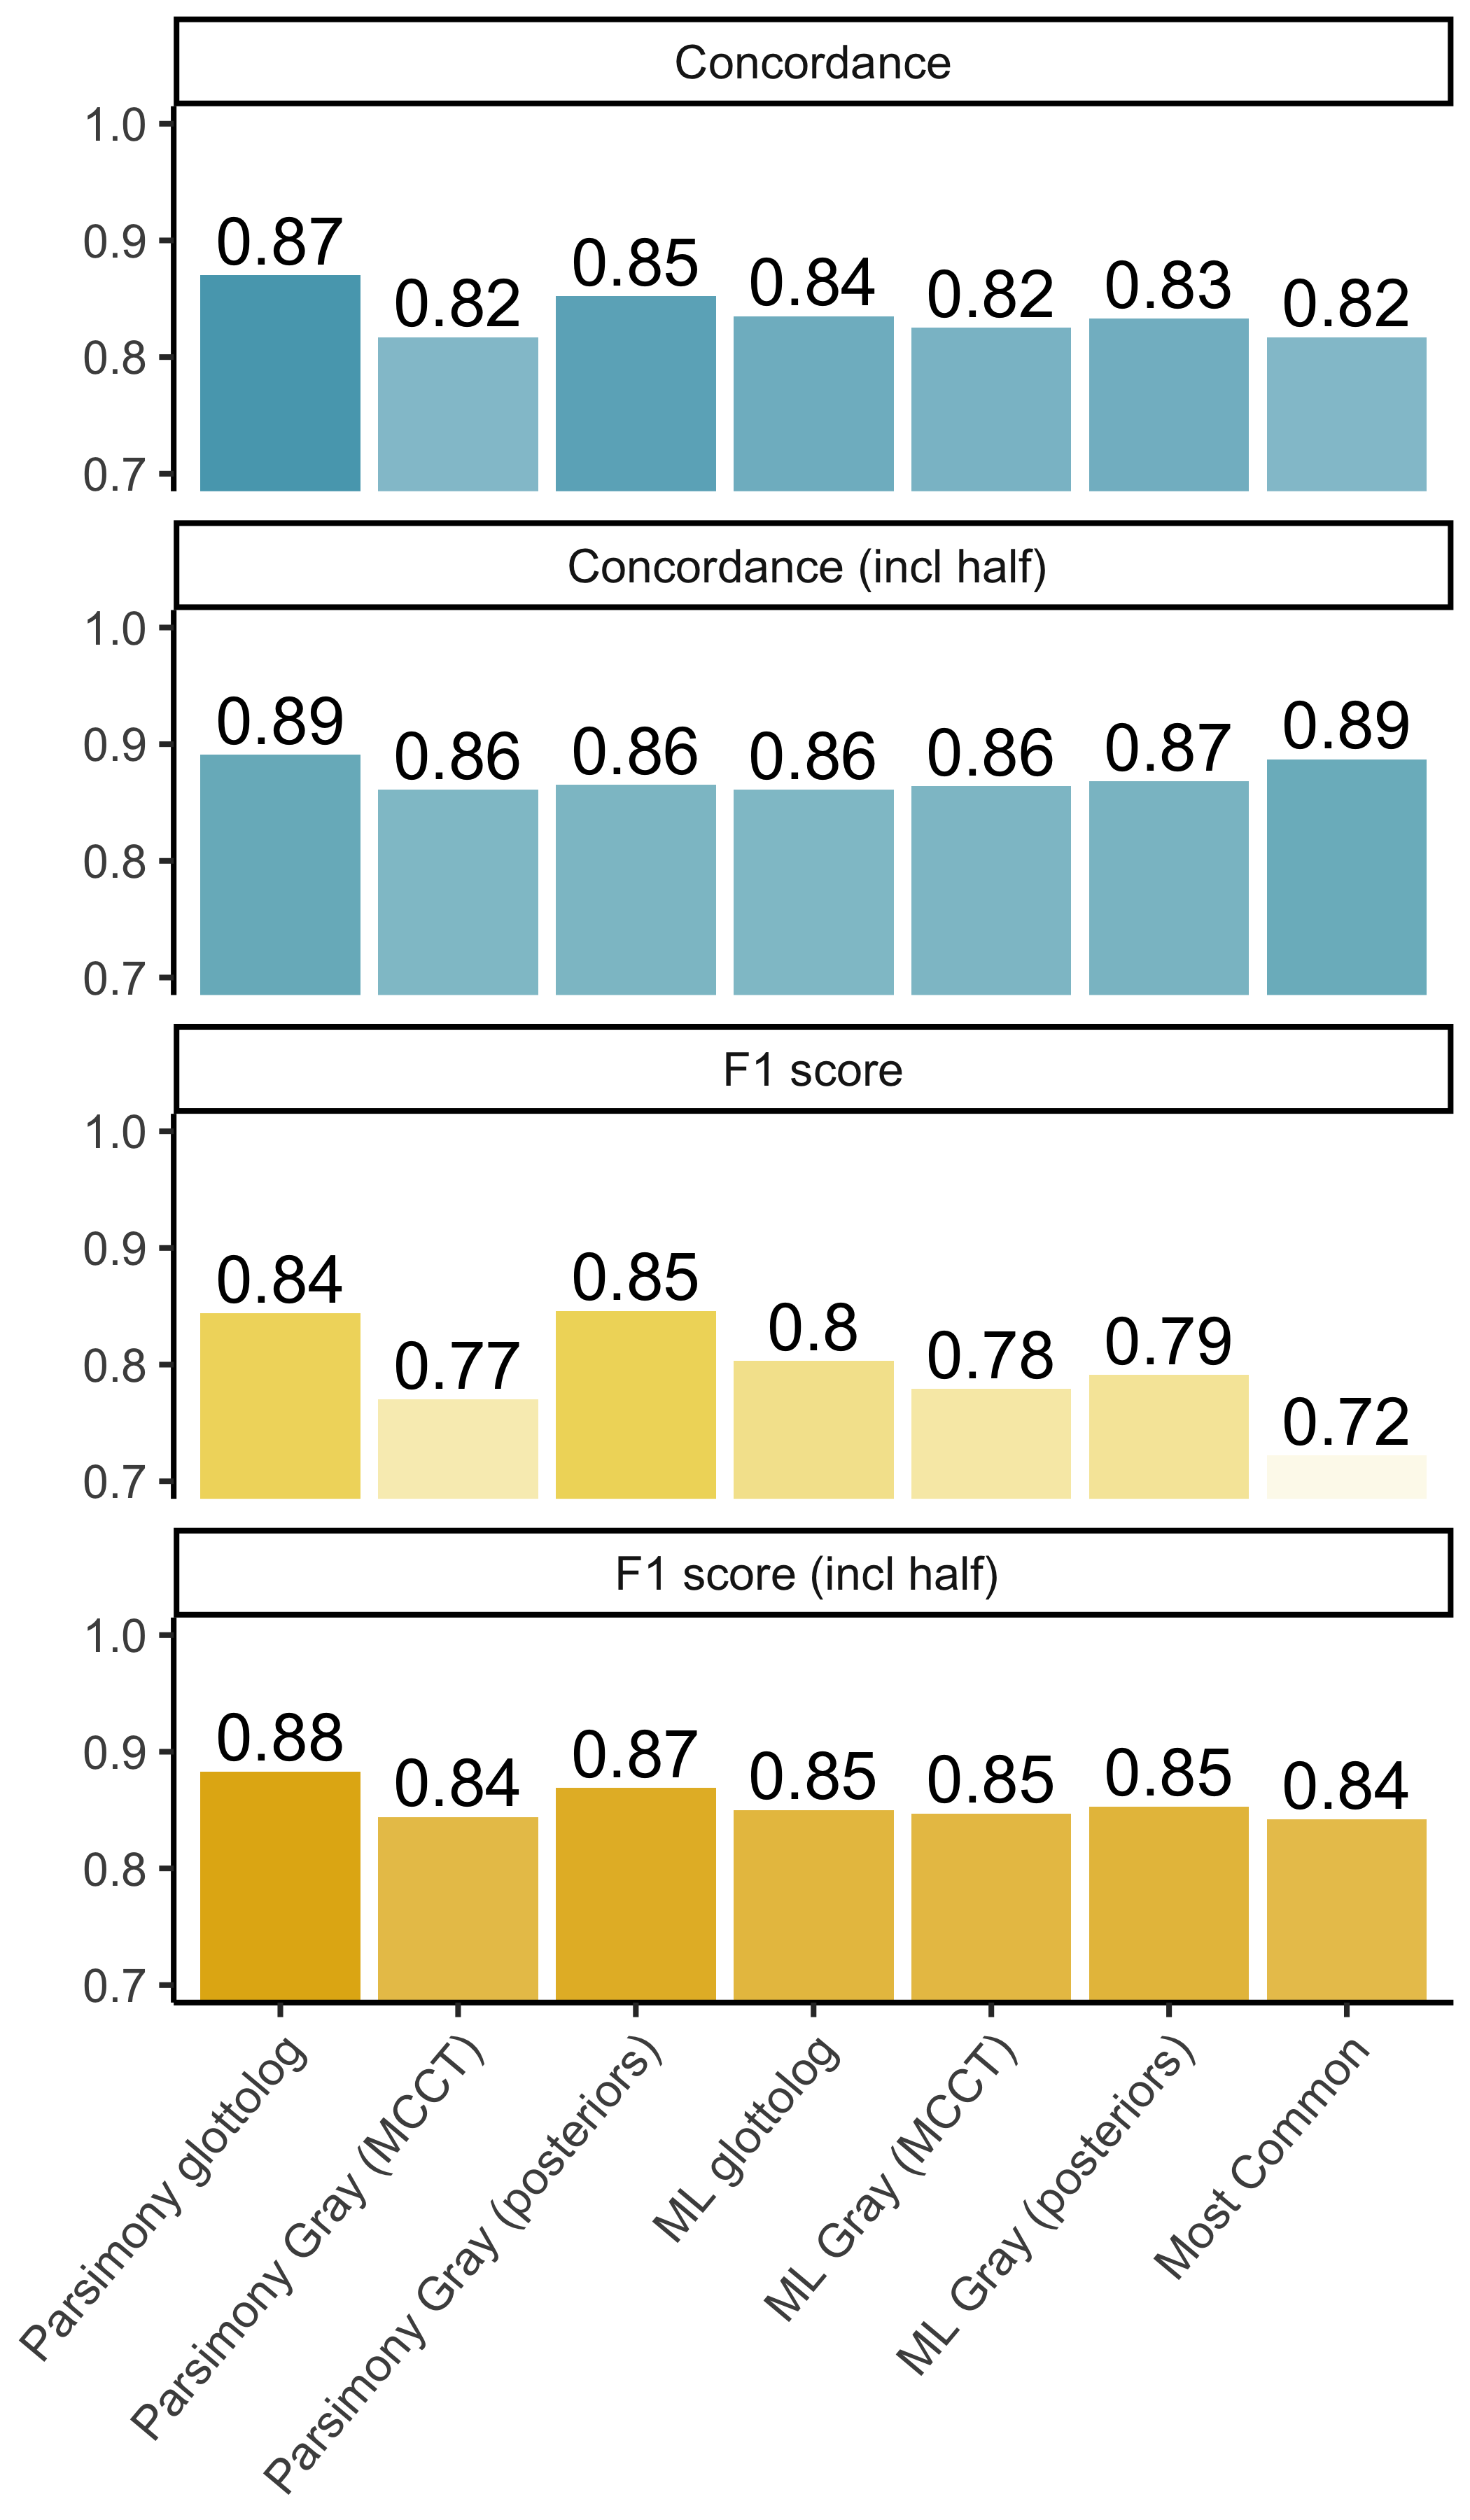
\includegraphics[width=11cm]{illustrations/plots_from_R/results/barplot_facet_scores.png}
\caption{\textbf{Barplots of concordance and F1-scores of each method.} NB that the y-axis starts from 0.7.}
\label{barplot_facet_results_incl_f1}
\end{figure}

Compared to the F1-scores from the lexical reconstruction of \citet{jager2018using}, all of the methods achieved higher scores. The highest (``best'') F1-score in \citet{jager2018using} was 0.79 (Austronesian language sample, Maximum Likelihood), and the worst was 0.44 (Indo-European, Minimal Lateral Networks). In this study, only statements about ancestral languages that could be mapped to Grambank-features were included. It is  possible that the study by \citet{jager2018using} had a greater overlap between all the reconstructions made by historical linguists and the meanings that they had data for. In that case, it is possible that the features that were possible to map to Grambank data were also those that Oceanic historical linguists are the most confident about -- hence the higher scores of agreement (quantified as F1-scores) compared to \citet{jager2018using}.

\FloatBarrier


\section{Mathematics of the F1-score including half-results}
\label{math_supp}

I am very grateful for the assistance of Stephen Mann in working out the mathematics of these scores as they incorporate the Half-results.

\subsection{Standard definitions}\label{sec:standard}

The F1-score is the harmonic mean of precision and recall \citep{van1979information}.

\begin{align*}
    F_1 &= 2\times\frac{\text{precision}\times\text{recall}}
            {\text{precision} + \text{recall}}\\
        &= \frac{\text{TP}}
            {\text{TP}+\frac{1}{2}\times(\text{FP}+\text{FN})}
\end{align*}

\begin{align*}
    \text{precision} 
        &= \frac{\text{TP}}
            {\text{TP}+\text{FP}}
\end{align*}

\begin{align*}
    \text{recall} 
        &= \frac{\text{TP}}
            {\text{TP}+\text{FN}}
\end{align*}

%%%%%%%%%%%
%%%%%%%%%%%
%%%%%%%%%%%
%%%%%%%%%%%
\subsection{Half-result definitions of precision and recall}\label{sec:halfsies}

The half-result-definitions of precision and recall add one half of the half-counts to the numerator, and all of the half-counts to the denominator:

\begin{equation*}
    \text{precision}_{\text{half}} 
        = \frac{\text{TP}+\frac{\text{H}}{2}}
            {\text{TP}+\text{FP}+\text{H}}
\end{equation*}

\begin{equation*}
    \text{recall}_{\text{half}}
        = \frac{\text{TP}+\frac{\text{H}}{2}}
            {\text{TP}+\text{FN}+\text{H}}
\end{equation*}

%%%%%%%%%%%
%%%%%%%%%%%
%%%%%%%%%%%
%%%%%%%%%%%
\subsection{The question}\label{sec:question}

We want to define $F_{1,\text{half}}$.
A natural way to do it would be to follow the rule defined above, i.e.

\begin{equation*}
    F_{1,\text{half?}} = \frac{\text{TP}+\frac{\text{H}}{2}}
            {\text{TP}+\frac{1}{2}\times(\text{FP}+\text{FN}) + \text{H}}
\end{equation*}

\noindent However, we want to ensure $F_{1,\text{half}}$ has the same relationship with $\text{precision}_{\text{half}}$ and $\text{recall}_{\text{half}}$ as $F_1$ has with precision and recall.
So we need to determine whether the following equation is true:

\begin{equation}\label{eq:question}
    2\times\frac{\text{precision}_{\text{half}}\times\text{recall}_{\text{half}}}
            {\text{precision}_{\text{half}} + \text{recall}_{\text{half}}}
    \stackrel{?}{=}
    \frac{\text{TP}+\frac{\text{H}}{2}}
            {\text{TP}+\frac{1}{2}\times(\text{FP}+\text{FN}) + \text{H}}
\end{equation}

%%%%%%%%%%%
%%%%%%%%%%%
%%%%%%%%%%%
%%%%%%%%%%%
\subsection{The proof}\label{sec:proof}

We will expand the left-hand side of \eqref{eq:question} and show it is equal to the right-hand side.
Let's forget about the $2\times$ for now (we will reintroduce it at the end).
Expanding the numerator gives:

\begin{equation*}
    \frac{\left(
        \text{TP}+\frac{\text{H}}{2}
    \right)\left(
        \text{TP}+\frac{\text{H}}{2}
    \right)}
    {\left(
        \text{TP} + \text{FP} + \text{H}
    \right)\left(
        \text{TP} + \text{FN} + \text{H}
    \right)}
\end{equation*}

\noindent Expanding the denominator gives:

\begin{align*}
    &\frac{\text{TP}+\frac{\text{H}}{2}}
    {\text{TP}+\text{FP}+\text{H}}
    +
    \frac{\text{TP}+\frac{\text{H}}{2}}
    {\text{TP}+\text{FN}+\text{H}}\\[1.5ex]
    &=
    %% Second line, left part
    %% Numerator
    \frac{\left(
        \text{TP}+\frac{\text{H}}{2}
    \right)\left(
        \text{TP}+\text{FN}+\text{H}
    \right)}
    %% Denominator
    {\left(
        \text{TP}+\text{FP}+\text{H}
    \right)\left(
        \text{TP}+\text{FN}+\text{H}
    \right)}
    +
    %% Second line, right part
    %% Numerator
    \frac{\left(
        \text{TP}+\frac{\text{H}}{2}
    \right)\left(
        \text{TP}+\text{FP}+\text{H}
    \right)}
    %% Denominator
    {\left(
        \text{TP}+\text{FN}+\text{H}
    \right)\left(
        \text{TP}+\text{FP}+\text{H}
    \right)}\\[1.5ex]
    %% Third line
    &=\frac{\left(
        \text{TP}+\frac{\text{H}}{2}
    \right)\left(
        2\times\text{TP} + \text{FP} + \text{FN} + 2\times\text{H}
    \right)}
    {\left(
        \text{TP}+\text{FP}+\text{H}
    \right)\left(
        \text{TP}+\text{FN}+\text{H}
    \right)}
\end{align*}

\noindent When we put the numerator back on top of the denominator, both of their respective denominators cancel out, because they are both $(\text{TP}+\text{FP}+\text{H})(\text{TP}+\text{FN}+\text{H})$.
So we end up with \emph{the numerator of the numerator} on top of \emph{the numerator of the denominator}, like so:

\begin{align*}
    &\frac{\left(
        \text{TP}+\frac{\text{H}}{2}
    \right)\left(
        \text{TP}+\frac{\text{H}}{2}
    \right)}
    {\left(
        \text{TP}+\frac{\text{H}}{2}
    \right)\left(
        2\times\text{TP} + \text{FP} + \text{FN} + 2\times\text{H}
    \right)}\\[1.5ex]
    &=
    \frac{\left(
        \text{TP}+\frac{\text{H}}{2}
    \right)}
    {2\times\text{TP} + \text{FP} + \text{FN} + 2\times\text{H}}
\end{align*}

\noindent Finally, we bring back the $2\times$ from the beginning:

\begin{align*}
    &2\times\frac{\left(
        \text{TP}+\frac{\text{H}}{2}
    \right)}
    {2\times\text{TP} + \text{FP} + \text{FN} + 2\times\text{H}}\\[1ex]
    &=
    \frac{\text{TP}+\frac{\text{H}}{2}}
    {\text{TP} + \frac{1}{2}\times(\text{FP} + \text{FN}) + \text{H}}
\end{align*}

\noindent And we have our suggested definition of $F_{1,\text{half}}$ as required.

\FloatBarrier


%


\section{Further details on the tree phylogeny}
\label{supp:tree_details}

The tree from \citet{grayetal_2009} contains duplicates in terms of glottocodes (see for example Nakanai). This is because it is a tree of word-lists for languages (doculects) rather than languages themselves. There are also some instances where multiple dialects of one language are included. For the analysis, only one tip per language was retained, based on which had best coverage in the underlying data for the tree (i.e., the Austronesian Basic Vocabulary Database, ABVD \citep{ABVD}). This means that duplicate glottocodes were reduced to one, be it due to multiple word-lists or dialects. The specific analytical choices are found in the following three R-scripts:

\begin{itemize}
\item Oceanic\_computational\_ASR/code/01\_requirements.R
\item Oceanic\_computational\_ASR/code/analysis\_scripts\_gray\_mcct/\\03\_get\_gray\_tree\_mcct.R
\item Oceanic\_computational\_ASR/code/analysis\_scripts\_gray\_all\_posterior/\\03\_process\_gray\_tree\_posteriors.R
\end{itemize}

For both Maximum Parsimony and Maximum Likelihood the tree were first pruned down to only languages where there is data in Grambank for each given feature, i.e., the ASR-analysis never contains tips with missing or ambiguous data. Missing data vary with features, so each analysis per tree and method differs in number of tips.

%For the further Maximum Parsimony analysis, tips representing languages where the data for a particular feature was missing were dropped for the analysis of that feature. For the Maximum Likelihood analysis, the value at such tips was converted to ambiguous. This is necessary because otherwise the rate of change across the different features would not be comparable in the Maximum Likelihood analysis.

Regarding branch lengths, most of the trees in the analysis are not ultrametric, i.e., the distances between the tips and the roots are not all the same. If we use trees to represent history and time, then an ultrametric, or near-Ultrametric, tree is a more reasonable representation of said histories when we assume that the languages at the tips existed at the same time. Fig \ref{fig:branch_lengths} illustrates different configurations of branch lengths using only Nuclear Polynesian languages. It is reasonable to assume that the data gathered on these languages represent similar time-slices to each other, i.e., the representation of Rapa Nui is not considerably ``younger'' as a language than Tongan. If the tips included ancient languages, such as Sanskrit or Akkadian, it may be possible for such tips to have a shorter distance to the root than the others. However, if the languages are of a similar ``age'', the tree ought to be ultrametric or near-ultrametric if we understand tree length as representing time.

The Glottolog genealogical classification follows common principles in historical linguistics by focusing on the validity of subgrouping, not branch lengths. The Glottolog 4.5 tree does not include any information about branch lengths. This is interpreted as the same as if all branches are of the same length (they are explicitly all set to 1 in the analysis). In order to illustrate what this entails, consider the difference between Figure \ref{glottolog_example_poly_1} and Figure \ref{glottolog_example_poly_grafen}. The first is the Glottolog tree of Nuclear Polynesian as found originally, i.e., with all branches of the same length (1). The second is a transformation of the first, it has been made ultrametric by Grafen's transform \citep{grafen1989phylogenetic}, which is one of several approaches to making a tree ultrametric in lieu of branch lengths directly from the data. The second tree is \emph{not} used in the analysis, it is included here only to illustrate how the same subgrouping of languages can be expressed when the branch lengths are changed. Transformations of branch lengths should be carried out with great care and with good reason. It is not clear what transformation of branch lengths in the Glottolog 4.5-tree is appropriate, which is why none has been carried out in the analysis of this paper. Keeping the Glottolog 4.5-tree lacking branch lengths may also be more true to historical linguistics methodology.

The branch lengths in the trees from \citet{grayetal_2009} are derived from the dynamics of the data -- the word-lists -- and certain priors regarding island settlement. The MCC-tree of \citet{grayetal_2009} is not ultrametric, but very close to it (see Fig \ref{gray_tree_branch_example}. After pruning to the subset that overlaps with Oceanic languages in Grambank (as described above), the difference between the tip with the largest distance to the root and the smallest is tiny (3.408377 -  3.408362). In the random sample of 100 from the 4,200 posteriors trees, the case is the same as with the MCCT -- they are not perfectly ultrametric but very close (see Fig \ref{gray_tree_branch_example_posteriors}. The trees from \citet{grayetal_2009} may not be perfectly ultrametric, but they are much more closer to ultrametric than the Glottolog tree, as can be seen by comparing the visualisations in Fig \ref{fig:branch_lengths}.

\begin{figure}[ht]
\centering
    \begin{subfigure}{0.5\linewidth}
      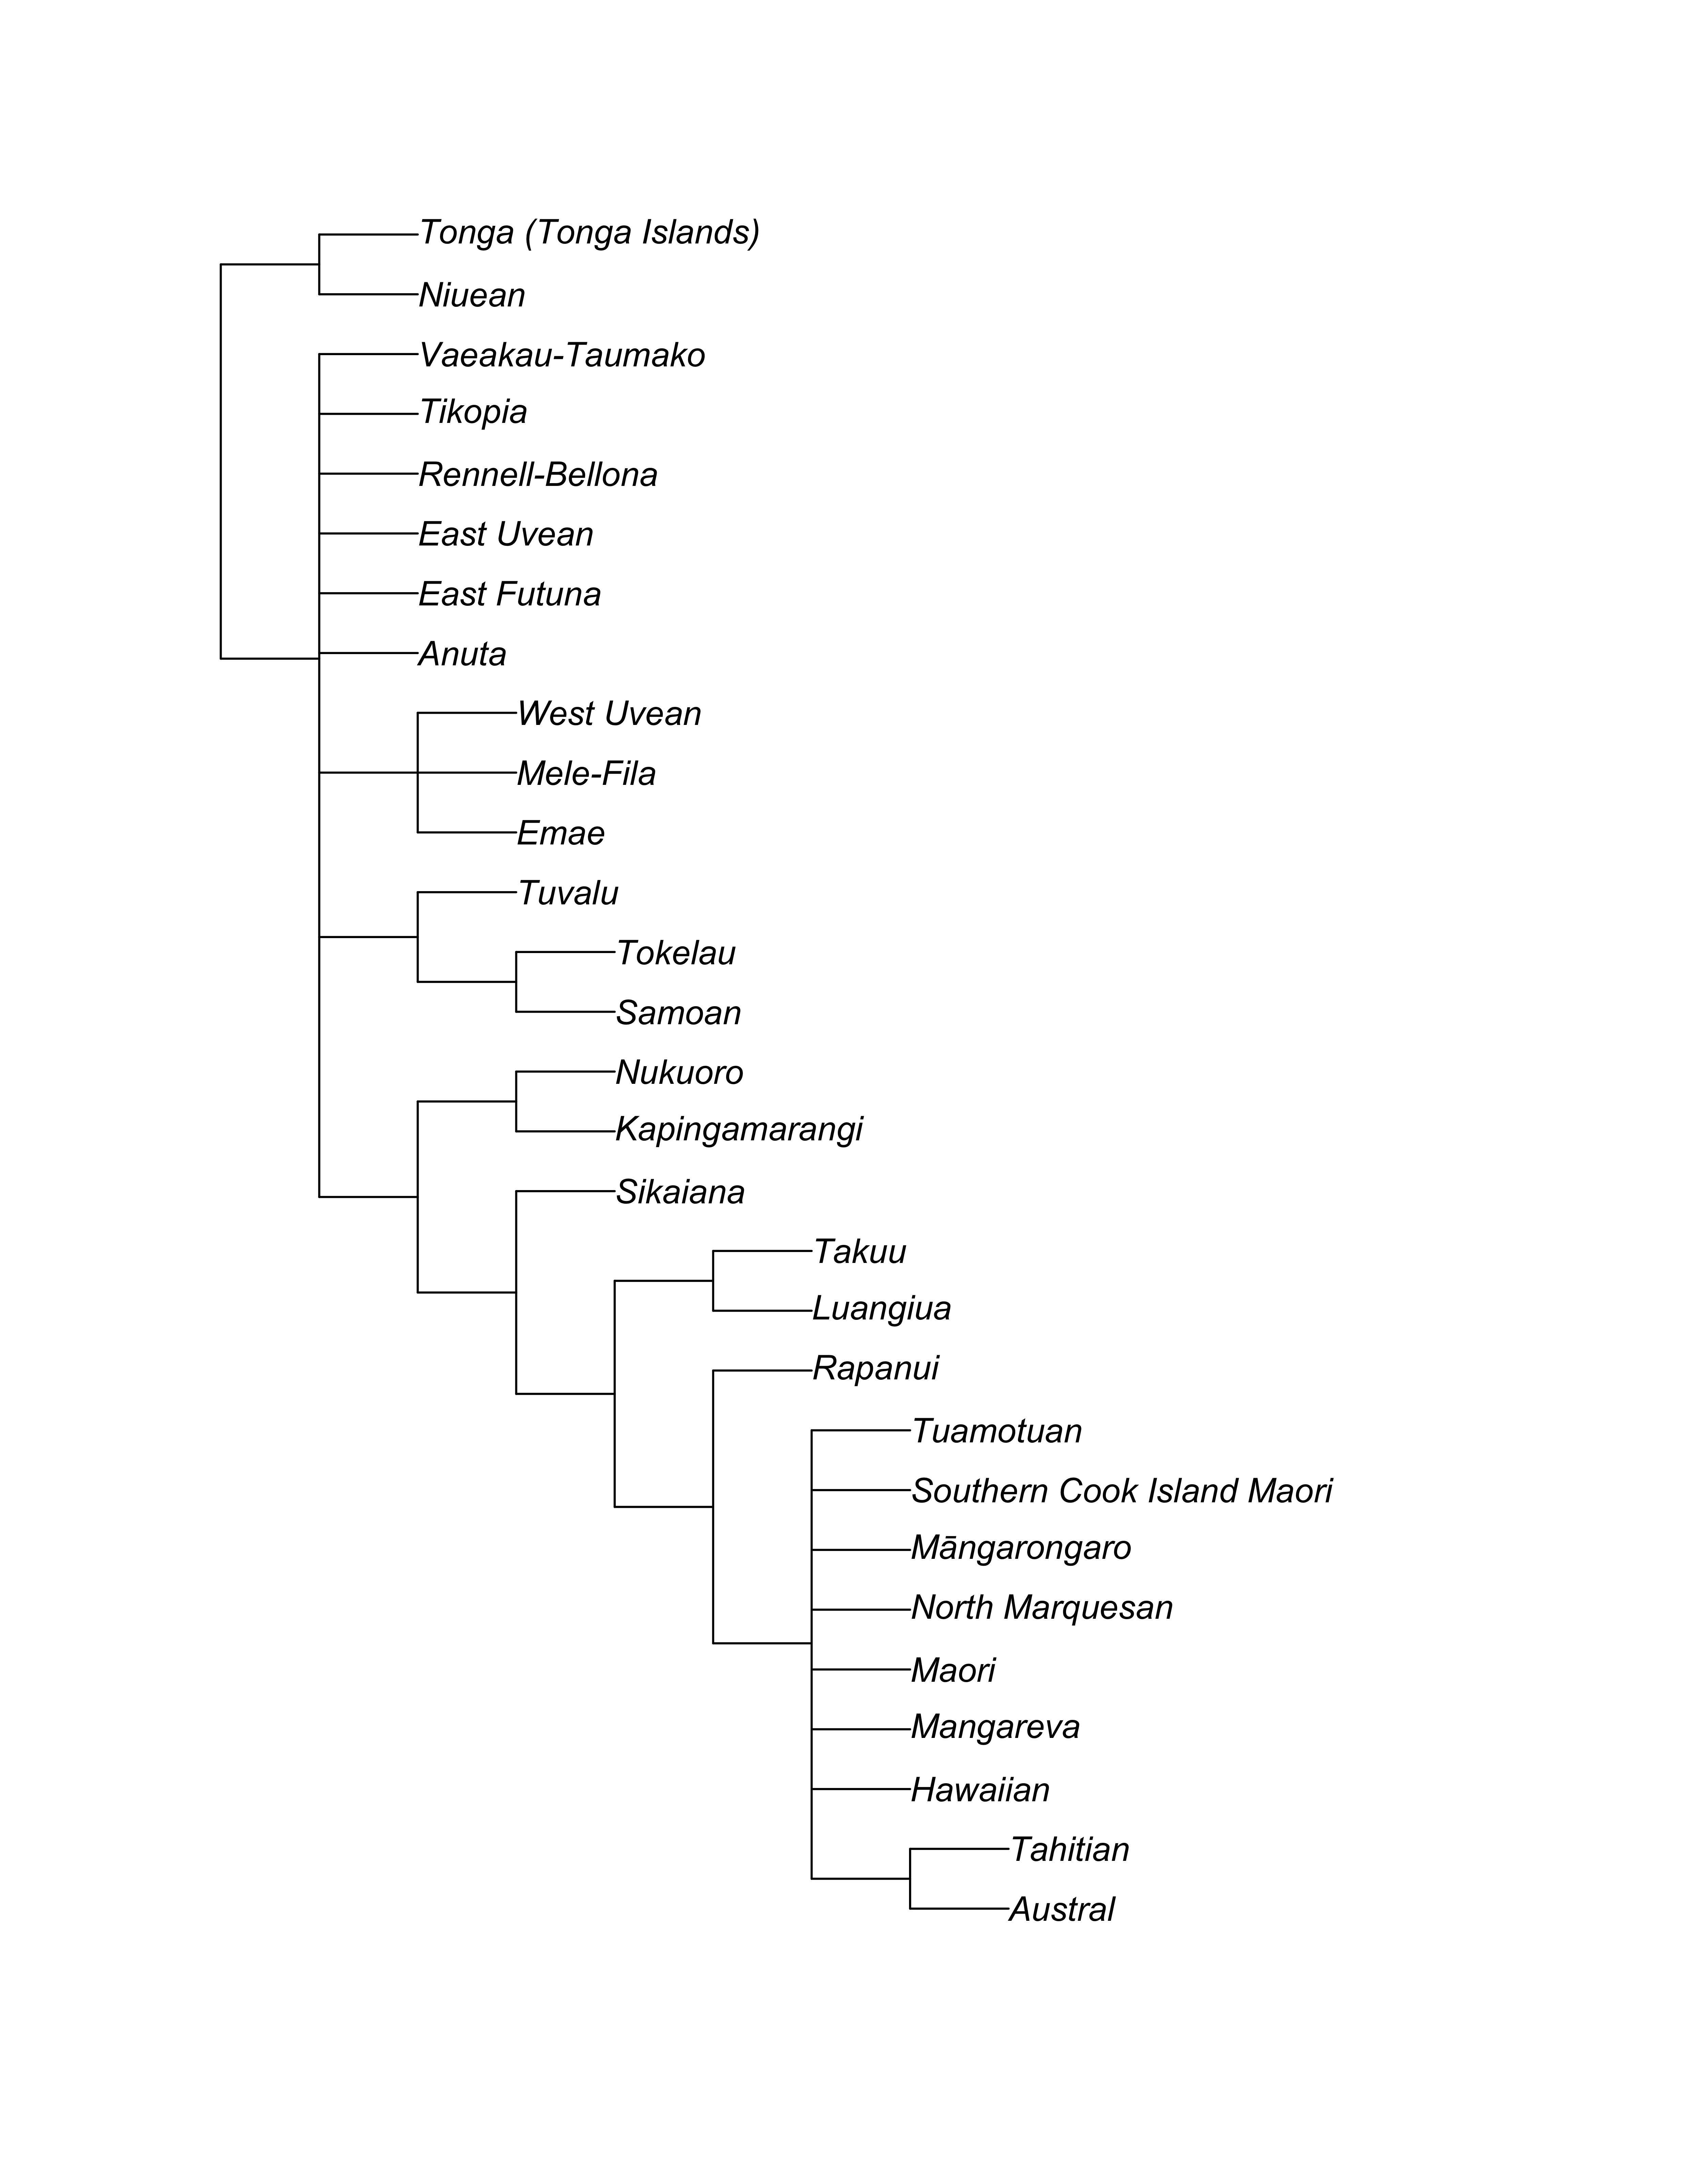
\includegraphics[width=\textwidth]{illustrations/plots_from_R/tree_plots/poly_tree_example_brlen_glottolog_1}
    \caption{Glottolog tree, all branches have the same length.}
    \label{glottolog_example_poly_1}
    \end{subfigure}
\hfil
    \begin{subfigure}{0.5\linewidth}
          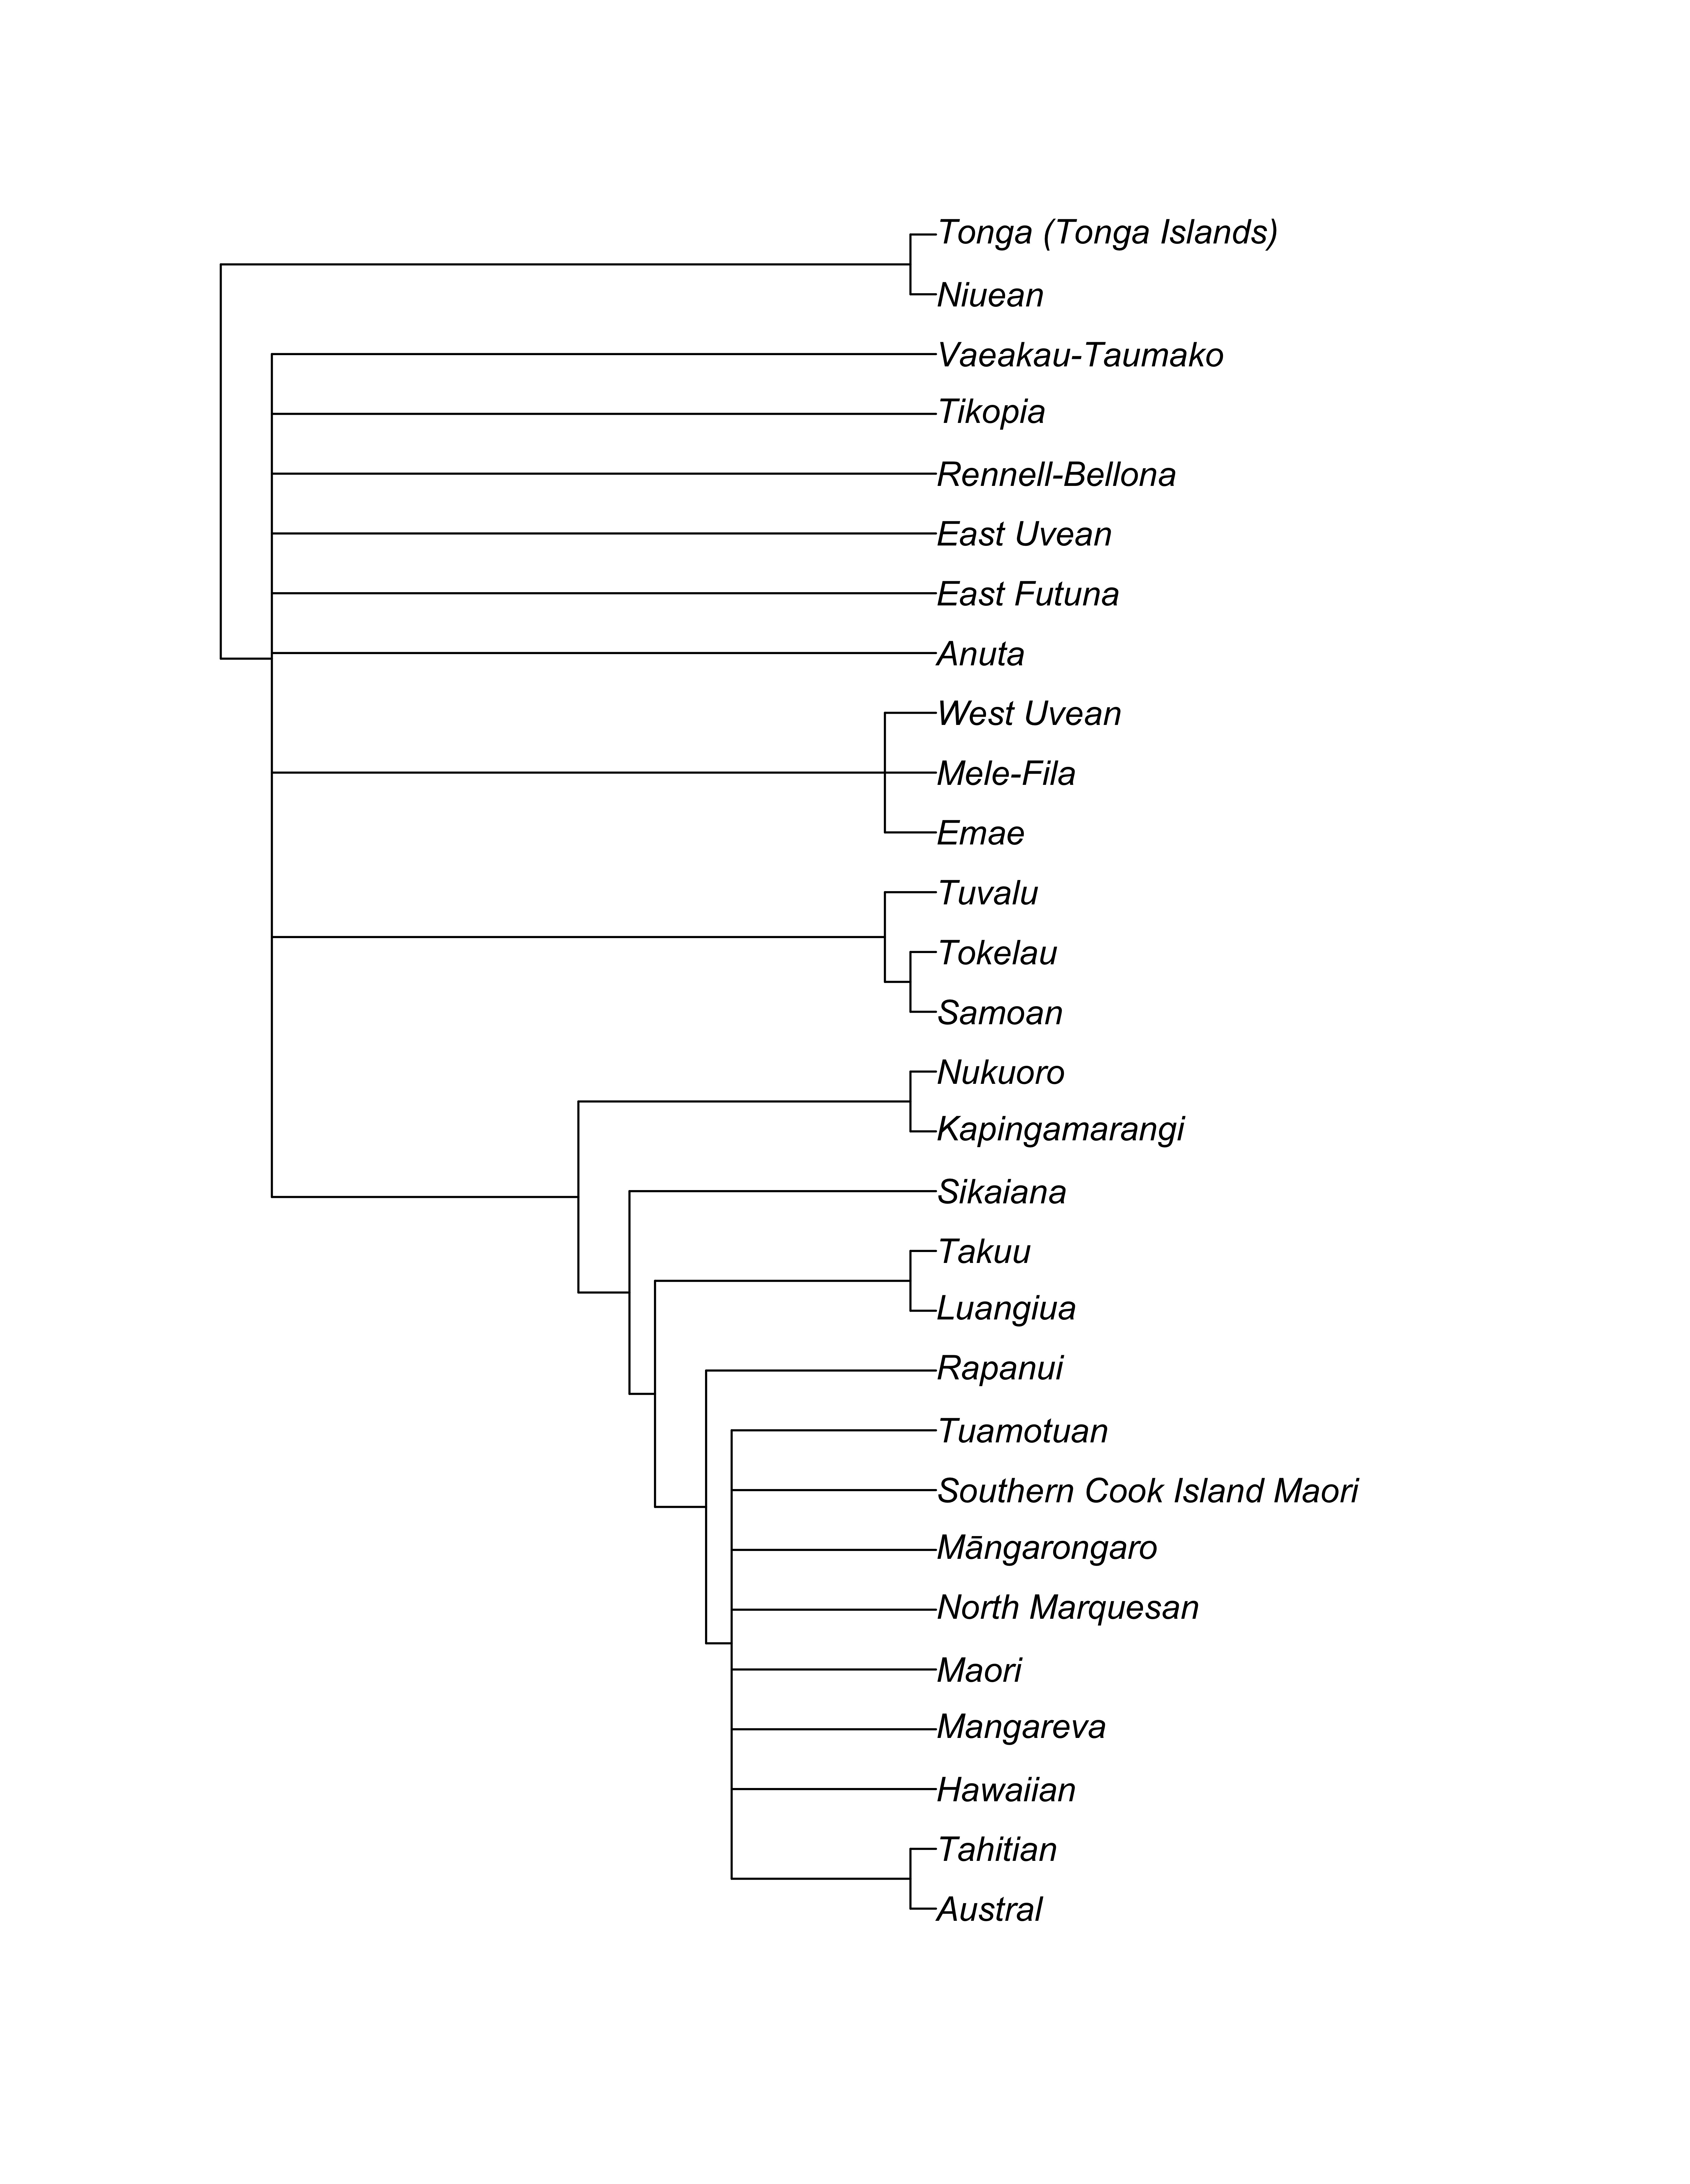
\includegraphics[width=\textwidth]{illustrations/plots_from_R/tree_plots/poly_tree_example_brlen_glottolog_grafen.png}
     \caption{Glottolog tree, made ultrametric with Grafen's method \citep{grafen1989phylogenetic}.}
      \label{glottolog_example_poly_grafen}
    \end{subfigure}

    \begin{subfigure}{0.5\linewidth}
          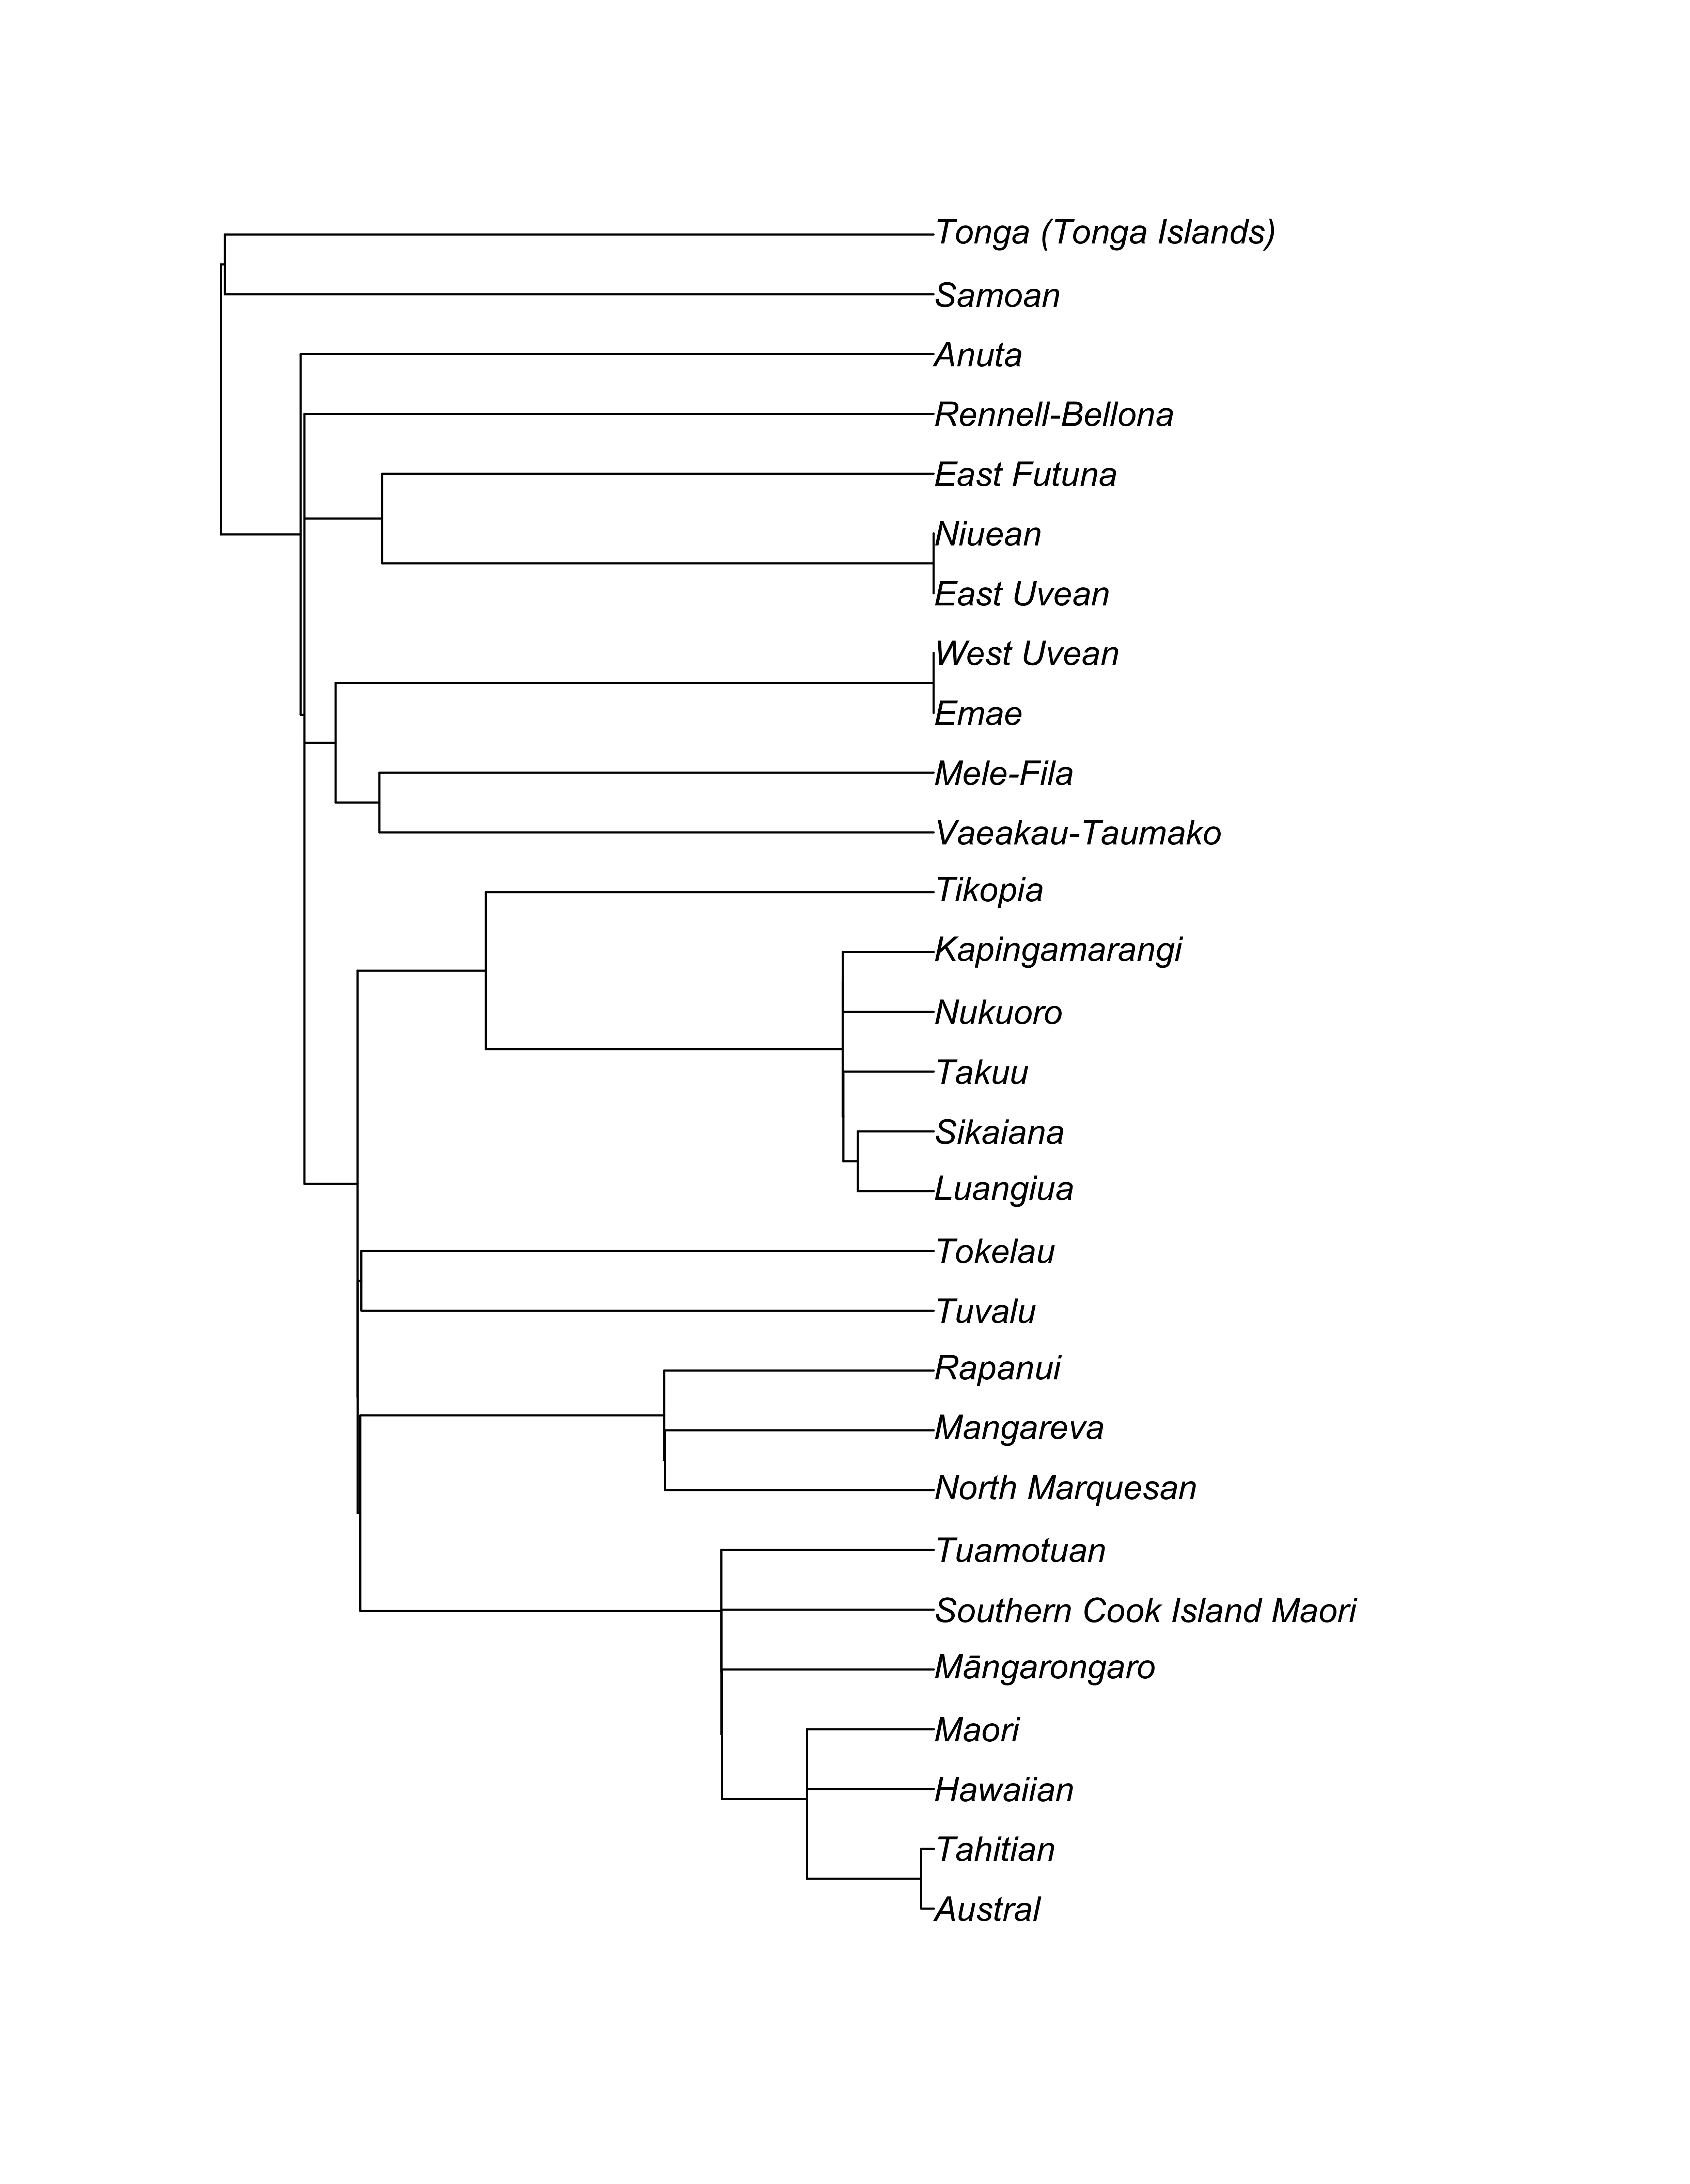
\includegraphics[width=\textwidth]{illustrations/plots_from_R/tree_plots/poly_tree_example_brlen_gray.png}
    \caption{\citet{grayetal_2009} MCCT.}
     \label{gray_tree_branch_example}
    \end{subfigure}
\hfil
    \begin{subfigure}{0.5\linewidth}
          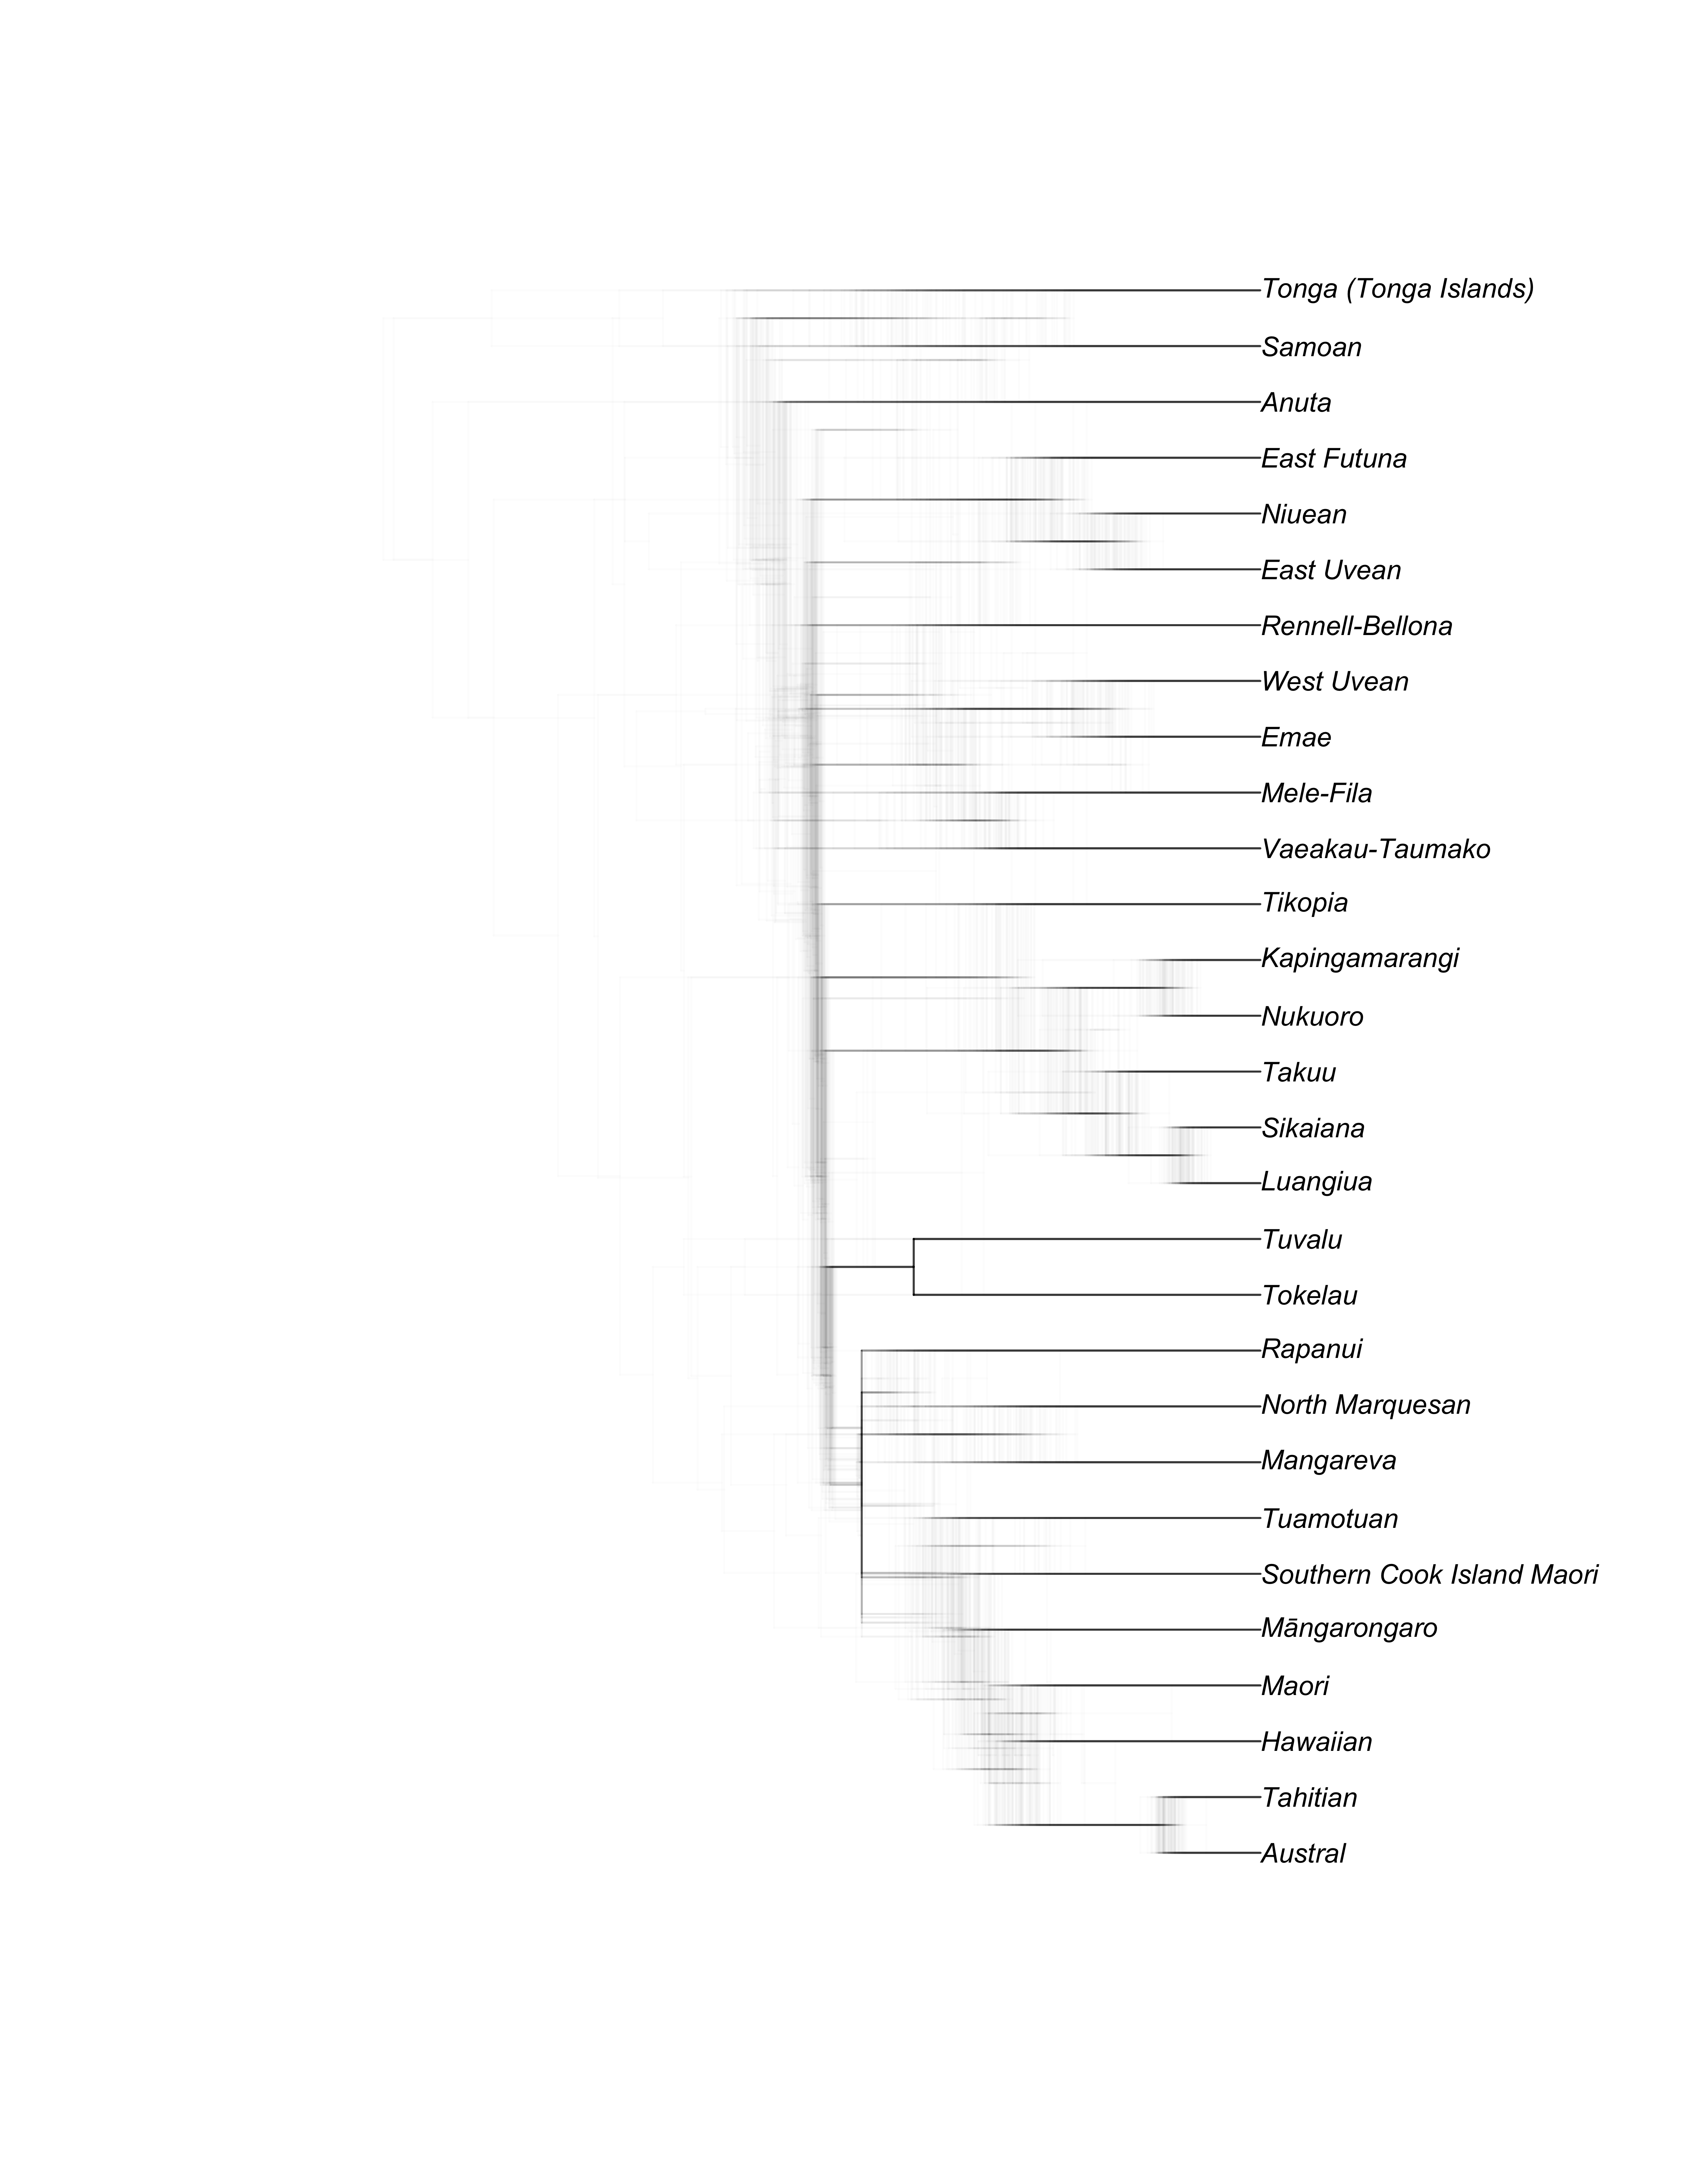
\includegraphics[width=\textwidth]{illustrations/plots_from_R/tree_plots/poly_tree_example_brlen_gray_posterios.png}
    \caption{\citet{grayetal_2009} posteriors tree (random sample of 100). The densitree-visualisation is in phylogram-style.}
     \label{gray_tree_branch_example_posteriors}
    \end{subfigure}
    
\caption{Four trees of Nuclear Polynesian, demonstrating branch lengths.}
    \label{fig:branch_lengths}
\end{figure}

Concerning binary splits, there are non-binary splits in the Glottolog 4.5 tree, the \citet{grayetal_2009} MCCT and in 64 of the 100 posterior trees. For this analysis, we have chosen to not resolve these polytomies into binary splits in order to stay as true as possible to the original phylogeny. There are branches of length 0 in the MCCT and posterior trees. It is not possible to collapse these into polytomies as this may in cases introduce basal polytomies. Instead, 0.00011 length was added to all branches. Doing this removes branches of length 0 while maintaining the relative lengths of all branches in the tree.

In some cases, pruning a given posterior tree to the relevant tips resulted in the tree becoming unrooted. In such cases, the tree was re-rooted using midpoint rooting \texttt{castor::root\_at\_midpoint()} \cite{R-castor}. There were 4 such cases in the random sample of posteriors trees (random seed = 147).

All of the wrangling of the trees is found in the data analysis R-scripts that accompany this paper.
\FloatBarrier    


\section{Further details on the Grambank coding of proto-languages }
\label{supp:proto_lg_coding}
Another example of how information in the publications was turned into Grambank feature coding relates to verbal markers encoding subjects and objects, as proposed by \citet{lynchrosscrowley_proto_grammar_oceanic} among others. In their book, there is a paper on reconstructions of grammar for Proto-Oceanic and in the section on the basic verb phrase we find the statement below:

\begin{quotation}
\noindent\emph{Attached to the verb root were a subject proclitic and, if the verb had a non-generic object, an object enclitic.} \end{quotation} \begin{flushright} \citet[83]{lynchrosscrowley_proto_grammar_oceanic} \end{flushright}

This statement, together with a verb schema provided in the section, support the notion that Proto-Oceanic had subject proclitics and object enclitics. We can also infer from this publication as a whole that the authors believe Proto-Oceanic in fact did \emph{not} have subject \emph{en}clitics and object \emph{pro}clitics. This second prediction relies on absence of evidence and is less strong than the first, but given that the whole paper is void of any description of object proclitics or subject enclitics being a possibility (including the verb schema) and argument structure is well-discussed, we may dare to make this leap. This information can be translated into the Grambank questionnaire by positing absence and presence for the six relevant features that concern argument marking on the verb (where S stands for subject of intransitive, A for subject of transitive and O for object; see table~\ref{example_HL_prediction_table}).

 %one of ste's favourite tables
\begin{table}
\caption{Example of predictions from historical linguistics as rendered in Grambank features.}
\label{example_HL_prediction_table}

\begin{tabular}{|p{3cm}| p{4.5cm}|  p{2.5cm}| p{2.5cm} | p{3cm} |p{2cm}| }
\hline
\textbf{Grambank ID} & \textbf{Question} & \textbf{Proto-language} & \textbf{Expert prediction} & \textbf{Reference} \\ 
\hline
GB089  &Can the S argument be indexed by a suffix/enclitic on the verb in the simple main clause? &Proto-Oceanic &Absent & \citet[498-499]{ross2004morphosyntactic}, \citet[83]{lynchrosscrowley_proto_grammar_oceanic} \\ \hline
GB090 &Can the S argument be indexed by a prefix/proclitic on the verb in the simple main clause? &Proto-Oceanic &Present &\citet[498-499]{ross2004morphosyntactic}, \citet[83]{lynchrosscrowley_proto_grammar_oceanic}  \\ \hline
GB091 &Can the A argument be indexed by a suffix/enclitic on the verb in the simple main clause? &Proto-Oceanic &Absent &\citet[498-499]{ross2004morphosyntactic}, \citet[83]{lynchrosscrowley_proto_grammar_oceanic} \\ \hline
GB092  &Can the A argument be indexed by a prefix/proclitic on the verb in the simple main clause? &Proto-Oceanic &Present &\citet[498-499]{ross2004morphosyntactic}, \citet[83]{lynchrosscrowley_proto_grammar_oceanic}  \\ \hline
GB093  &Can the P argument be indexed by a suffix/enclitic on the verb in the simple main clause? &Proto-Oceanic &Present &\citet[498-499]{ross2004morphosyntactic}, \citet[83]{lynchrosscrowley_proto_grammar_oceanic} \\ \hline
GB094  &Can the P argument be indexed by a prefix/proclitic on the verb in the simple main clause? &Proto-Oceanic &Absent & \citet[498-499]{ross2004morphosyntactic}, \citet[83]{lynchrosscrowley_proto_grammar_oceanic} \\ \hline
\end{tabular}
\end{table}



\FloatBarrier
%\section{Table of new predictions}
%\label{asr_table_extra}
%\begin{landscape}
%% latex table generated in R 4.2.3 by xtable 1.8-4 package
% Mon Jun 12 21:27:07 2023
\begin{longtable}{p{1.5cm}p{2.5cm}p{2.5cm}p{2.5cm}p{2.5cm}p{2.5cm}p{2.5cm}p{2.5cm}}
  \toprule
Feature\_ID & Glottolog Parsimony & Gray parismony -MCCT & Gray parismony -posteriors & Glottolog ML & Gray ML -MCCT & Gray ML -posteriors & Most Common \\ 
  \midrule
GB024a & Present & Present & Present & Present & Present & Present & Present \\ 
  GB024b & Present & Present & Present & Present & Present & Present & Present \\ 
  GB024b & Present & Present & Present & Present & Present & Present & Present \\ 
  GB024b & Present & Present & Present & Present & Present & Present & Present \\ 
  GB024b & Present & Present & Present & Present & Present & Present & Absent \\ 
  GB025a & Present & Present & Present & Present & Present & Present & Present \\ 
  GB025b & Present & Present & Present & Present & Present & Present & Present \\ 
  GB025b & Present & Present & Present & Present & Present & Present & Present \\ 
  GB065b & Present & Present & Present & Present & Present & Present & Present \\ 
  GB065b & Present & Present & Present & Present & Present & Present & Present \\ 
  GB065b & Present & Present & Present & Present & Present & Present & Present \\ 
  GB130a & Present & Present & Present & Present & Present & Present & Present \\ 
  GB130b & Present & Present & Present & Present & Present & Present & Present \\ 
  GB193b & Present & Present & Present & Present & Present & Present & Present \\ 
  GB193b & Present & Present & Present & Present & Present & Present & Present \\ 
  GB203b & Present & Present & Present & Present & Present & Present & Present \\ 
  GB203b & Present & Present & Present & Present & Present & Present & Present \\ 
  GB203b & Present & Present & Present & Present & Present & Present & Present \\ 
  GB203b & Present & Present & Present & Present & Present & Present & Present \\ 
  GB020 & Present & Present & Present & Present & Present & Present & Present \\ 
  GB021 & Present & Present & Present & Present & Present & Present & Present \\ 
  GB022 & Present & Present & Present & Present & Present & Present & Present \\ 
  GB027 & Present & Present & Present & Present & Present & Present & Present \\ 
  GB028 & Present & Present & Present & Present & Present & Present & Present \\ 
  GB028 & Present & Present & Present & Present & Present & Present & Present \\ 
  GB031 & Present & Present & Present & Present & Present & Present & Present \\ 
  GB031 & Present & Present & Present & Present & Present & Present & Present \\ 
  GB035 & Present & Present & Present & Present & Present & Present & Present \\ 
  GB035 & Present & Present & Present & Present & Present & Present & Present \\ 
  GB047 & Present & Present & Present & Present & Present & Present & Present \\ 
  GB047 & Present & Present & Present & Present & Present & Present & Present \\ 
  GB047 & Present & Present & Present & Present & Present & Present & Present \\ 
  GB057 & Present & Present & Present & Present & Present & Present & Present \\ 
  GB059 & Present & Present & Present & Present & Present & Present & Present \\ 
  GB059 & Present & Present & Present & Present & Present & Present & Present \\ 
  GB068 & Present & Present & Present & Present & Present & Present & Present \\ 
  GB068 & Present & Present & Present & Present & Present & Present & Present \\ 
  GB068 & Present & Present & Present & Present & Present & Present & Present \\ 
  GB074 & Present & Present & Present & Present & Present & Present & Present \\ 
  GB074 & Present & Present & Present & Present & Present & Present & Present \\ 
  GB079 & Present & Present & Present & Present & Present & Present & Present \\ 
  GB079 & Present & Present & Present & Present & Present & Present & Present \\ 
  GB080 & Present & Present & Present & Present & Present & Present & Present \\ 
  GB080 & Present & Present & Present & Present & Present & Present & Present \\ 
  GB093 & Present & Present & Present & Present & Present & Present & Absent \\ 
  GB113 & Present & Present & Present & Present & Present & Present & Present \\ 
  GB124 & Present & Present & Present & Present & Present & Present & Present \\ 
  GB124 & Present & Present & Present & Present & Present & Present & Present \\ 
  GB126 & Present & Present & Present & Present & Present & Present & Present \\ 
  GB126 & Present & Present & Present & Present & Present & Present & Present \\ 
  GB126 & Present & Present & Present & Present & Present & Present & Present \\ 
  GB126 & Present & Present & Present & Present & Present & Present & Present \\ 
  GB131 & Present & Present & Present & Present & Present & Present & Present \\ 
  GB134 & Present & Present & Present & Present & Present & Present & Present \\ 
  GB134 & Present & Present & Present & Present & Present & Present & Present \\ 
  GB134 & Present & Present & Present & Present & Present & Present & Present \\ 
  GB134 & Present & Present & Present & Present & Present & Present & Present \\ 
  GB135 & Present & Present & Present & Present & Present & Present & Present \\ 
  GB135 & Present & Present & Present & Present & Present & Present & Present \\ 
  GB135 & Present & Present & Present & Present & Present & Present & Present \\ 
  GB135 & Present & Present & Present & Present & Present & Present & Present \\ 
  GB139 & Present & Present & Present & Present & Present & Present & Present \\ 
  GB139 & Present & Present & Present & Present & Present & Present & Present \\ 
  GB139 & Present & Present & Present & Present & Present & Present & Present \\ 
  GB155 & Present & Present & Present & Present & Present & Present & Present \\ 
  GB155 & Present & Present & Present & Present & Present & Present & Present \\ 
  GB158 & Present & Present & Present & Present & Present & Present & Present \\ 
  GB158 & Present & Present & Present & Present & Present & Present & Present \\ 
  GB158 & Present & Present & Present & Present & Present & Present & Present \\ 
  GB159 & Present & Present & Present & Present & Present & Present & Present \\ 
  GB159 & Present & Present & Present & Present & Present & Present & Present \\ 
  GB159 & Present & Present & Present & Present & Present & Present & Present \\ 
  GB254 & Present & Present & Present & Present & Present & Present & Present \\ 
  GB254 & Present & Present & Present & Present & Present & Present & Present \\ 
  GB254 & Present & Present & Present & Present & Present & Present & Present \\ 
  GB254 & Present & Present & Present & Present & Present & Present & Present \\ 
  GB257 & Present & Present & Present & Present & Present & Present & Present \\ 
  GB257 & Present & Present & Present & Present & Present & Present & Present \\ 
  GB257 & Present & Present & Present & Present & Present & Present & Present \\ 
  GB257 & Present & Present & Present & Present & Present & Present & Present \\ 
  GB299 & Present & Present & Present & Present & Present & Present & Present \\ 
  GB299 & Present & Present & Present & Present & Present & Present & Present \\ 
  GB301 & Present & Present & Present & Present & Present & Present & Present \\ 
  GB301 & Present & Present & Present & Present & Present & Present & Present \\ 
  GB301 & Present & Present & Present & Present & Present & Present & Present \\ 
  GB304 & Present & Present & Present & Present & Present & Present & Present \\ 
  GB318 & Present & Present & Present & Present & Present & Present & Present \\ 
  GB326 & Present & Present & Present & Present & Present & Present & Present \\ 
  GB326 & Present & Present & Present & Present & Present & Present & Present \\ 
  GB326 & Present & Present & Present & Present & Present & Present & Present \\ 
  GB326 & Present & Present & Present & Present & Present & Present & Present \\ 
  GB327 & Present & Present & Present & Present & Present & Present & Present \\ 
  GB327 & Present & Present & Present & Present & Present & Present & Present \\ 
  GB327 & Present & Present & Present & Present & Present & Present & Present \\ 
  GB333 & Present & Present & Present & Present & Present & Present & Present \\ 
  GB333 & Present & Present & Present & Present & Present & Present & Present \\ 
  GB333 & Present & Present & Present & Present & Present & Present & Present \\ 
  GB421 & Present & Present & Present & Present & Present & Present & Half \\ 
  GB433 & Present & Present & Present & Present & Present & Present & Absent \\ 
  GB519 & Present & Present & Present & Present & Present & Present & Present \\ 
  GB519 & Present & Present & Present & Present & Present & Present & Present \\ 
  GB520 & Present & Present & Present & Present & Present & Present & Present \\ 
  GB521 & Present & Present & Present & Present & Present & Present & Present \\ 
  GB521 & Present & Present & Present & Present & Present & Present & Present \\ 
  GB522 & Present & Present & Present & Present & Present & Present & Present \\ 
   \bottomrule
\caption{Table showing predictions where the six MP and ML methods agree on presence} 
\label{extra_predictions_table}
\end{longtable}

%\end{landscape}

%\section{Supplementary Figures}
%\label{supp:supplementary _figures}

%\section*{Summaries in German and French}

\newpage
\section{Appendix bibliography}
\bibliographystyle{unified}
\bibliography{ASR_Oceanic, bib_from_r/used_pkgs}




\end{document}